\documentclass{jarticle}
\usepackage[dvipdfm,bookmarks=true,bookmarksnumbered=true,bookmarkstype=toc]{hyperref}
\ifnum 42146=\euc"A4A2 \AtBeginDvi{\special{pdf:tounicode EUC-UCS2}}\else
\AtBeginDvi{\special{pdf:tounicode 90ms-RKSJ-UCS2}}\fi

%%% 余白の定義 %%%
\paperwidth 597pt
\paperheight 845pt
\hoffset -14.0pt
\voffset 14.5pt
 \oddsidemargin 0.0pt
 \evensidemargin 0.0pt
 \topmargin 0.0pt
 \headheight 0.0pt
 \headsep 0.0pt
\textheight 671.0pt
\textwidth 480.5pt
 \marginparsep 0.0pt
 \marginparwidth 0.0pt
 \footskip 15.0pt

\usepackage{amsmath}
\usepackage{amssymb}
\usepackage{amsthm}
\usepackage{ascmac}
\usepackage{boites}
\usepackage{color}
\usepackage{graphicx}
\usepackage{listings}
\usepackage{misc/jlisting}
\usepackage{makeidx}
\usepackage{multicol}
\usepackage{pxrubrica}
\usepackage{url}
\usepackage{wrapfig}

%%% 式番号に節番号を付与 %%%
\makeatletter
 \renewcommand{\theequation}{\thesection.\arabic{equation}}
 \@addtoreset{equation}{section}
\makeatother

%%% 図番号に節番号を付与 %%%
\makeatletter
 \renewcommand{\thefigure}{\thesection.\arabic{figure}}
 \@addtoreset{figure}{section}
\makeatother

%%% 表番号に節番号を付与 %%%
\makeatletter
 \renewcommand{\thetable}{\thesection.\arabic{table}}
 \@addtoreset{table}{section}
\makeatother

%%% 注釈 %%%
% \Notes{内容}
\newcounter{notesNum}
\newcommand{\Notes}[1]{\footnote [\arabic{notesNum}]{#1}\stepcounter{notesNum}}

%%% 索引 %%%
% \IND{項目}{こうもく}
% \Ind{Item}
\newcommand{\IND}[2]{\textbf{#1\index{#2@#1}}}
\newcommand{\Ind}[1]{\IND{#1}{#1}}

%%% theorem %%%
\theoremstyle{definition}
\newtheorem{prop}{命題}[section]
\newtheorem{theo}[prop]{定理}
\newtheorem{defi}[prop]{定義}
\newtheorem{lemm}[prop]{補題}
\newtheorem{coro}[prop]{系}
\newtheorem{conj}[prop]{予想}
\newtheorem{exam}[prop]{例}
\newtheorem{algo}[prop]{アルゴリズム}
\renewcommand{\qedsymbol}{(証明終)}
\renewcommand{\proofname}{\bfseries 証明}

% \begin{Prop}{Title}{label}
\newenvironment{Prop}[2]{\begin{prop}[#1]\label{prop:#2}}{\end{prop}}
\newenvironment{Theo}[2]{\begin{theo}[#1]\label{theo:#2}}{\end{theo}}
\newenvironment{Defi}[2]{\begin{defi}[#1]\label{defi:#2}}{\end{defi}}
\newenvironment{Lemm}[2]{\begin{lemm}[#1]\label{lemm:#2}}{\end{lemm}}
\newenvironment{Coro}[2]{\begin{coro}[#1]\label{coro:#2}}{\end{coro}}
\newenvironment{Conj}[2]{\begin{conj}[#1]\label{conj:#2}}{\end{conj}}
\newenvironment{Exam}[2]{\begin{exam}[#1]\label{exam:#2}}{\end{exam}}

%%% アルゴリズム %%%
% \Algo{Title}{label}{fileName}
\newcommand{\Algo}[3]{\begin{algo}[#1]\label{algo:#2}\footnotesize{#3}\end{algo}\vspace{-3.3mm}\lstinputlisting{src/#2.py}}

% 参照
\newcommand{\rProp}[1]{命題\ref{prop:#1}}
\newcommand{\rTheo}[1]{定理\ref{theo:#1}}
\newcommand{\rDefi}[1]{定義\ref{defi:#1}}
\newcommand{\rLemm}[1]{補題\ref{lemm:#1}}
\newcommand{\rCoro}[1]{系\ref{coro:#1}}
\newcommand{\rExam}[1]{例\ref{exam:#1}}
\newcommand{\rAlgo}[1]{アルゴリズム\ref{algo:#1}}

% proof環境
\newenvironment{prProof}[1]{\begin{proof}[\rProp{#1}の証明]}{\end{proof}}
\newenvironment{thProof}[1]{\begin{proof}[\rTheo{#1}の証明]}{\end{proof}}
\newenvironment{lmProof}[1]{\begin{proof}[\rLemm{#1}の証明]}{\end{proof}}
\newenvironment{crProof}[1]{\begin{proof}[\rCoro{#1}の証明]}{\end{proof}}

%プログラム挿入の設定
\lstset{
    language = Python,
    breaklines = true,
    breakindent = 10pt,
    basicstyle = \ttfamily\footnotesize,
    commentstyle = {\color[cmyk]{1,0.4,1,0}},
    classoffset = 0,
    keywordstyle = {\bfseries \color[cmyk]{0,1,0,0}},
    stringstyle = {\ttfamily \color[rgb]{0,0,1}},
    frame = single,
    framesep = 5pt,
    numberstyle = \tiny,
    tabsize = 4,
    showstringspaces=false,
}

\title{素数判定法と素因数分解アルゴリズム}
\author{}
\date{}
\makeindex
\begin{document}
\setcounter{notesNum}{1}
\maketitle
\begin{multicols}{2}
\setcounter{tocdepth}{2}
\tableofcontents
\end{multicols}
\newpage

\section{整数と素数、そして群}
\subsection{数論の最初の一歩}
まずは、素数とは何かをはっきりさせよう。
\IND{素数}{そすう}(prime)とは、1より大きな整数で、1とそれ自身以外では割り切ることができない数である。
具体的には、$2,3,5,7,11\ldots$などがそうである。

定義をうろ覚えの内は、「1は素数なのか?」と訊かれると戸惑ってしまいがちだが、1は素数ではない。
定義に立ち帰ってみると、\textbf{1より大きい}とわざわざ仲間外れにしていることがその根拠だ。
\kenten{1を作為的に素数から除外する}のは、後で述べる素因数分解の一意性を説明する上で都合が良いからであるが、ここでモヤっとする初学者が多いことも確かだ。
\IND{定義}{ていき}(definition)とは、概念に対する単なる「名付け」に過ぎない。
夜空に瞬く、ある星たちを「はくちょう座」と呼ぶことに、何ら物理法則が関与しないように、素数もまた人類が認識しやすいように切り取られた一つの概念に過ぎない。

「定義」について理解したところで、どのような数が素数なのか、ということを確認したい。

\begin{itemize}
 \item $2, 3, 5, 7, 11, 13, 17, 19, 23, 29, 31, 37, 41, 43, 47$は50以下のすべての素数である。
 \item $4, 12, 99$は素数ではない。なぜならば、それぞれ$2, 3, 11$で割り切れるからである。
\end{itemize}

素数でない整数を、いちいち「素数ではない整数」などと呼ぶことは不便だ\Notes{不便だからこそ、「定義する」という行為が行われるのである。}。
そこで、$1$でも素数でもない自然数は\IND{合成数}{こうせいすう}(composite number)と呼ぶこととする。

\IND{整数}{せいすう}(integer)と\IND{自然数}{しせんすう}(natural number)も慣れていないと\ruby{躓}{つまづ}いてしまう。
整数とは$\ldots,-2,-1,0,1,2,\ldots$と続く数で、自然数は$1,2,3,\ldots$と続く数である\Notes{自然数にゼロを含める流儀もあるが、本稿では含めないとする}。
それぞれ、$\mathbb{Z}$と$\mathbb{N}$という記号で書くこともあるが、記号の氾濫は混乱を招くだろうし、適宜補足するから、一旦読み飛ばしてもいい。

素数が発明されたのは、数の最小単位としての意味合いがある。
人類は物質の最小単位を夢想し、原子や素粒子を見つけてきたが、同じように、$1,2,3,4,\ldots$と続く自然数を掛け算でバラバラにすると、素数が現れる。

\begin{Theo}{\IND{素因数分解の一意性}{そいんすうふんかいのいちいせい}, unique factorization theorem}{unique_factorization_theorem}
$1$以外の正整数\Notes{正整数、あるいは非負整数は、その名の通り$1,2,3,\ldots$と続く数であり、ゼロを除いたときの自然数と同じだ。混乱を招くが、同じ概念に対して複数の用語があてがわれていることは往々にしてある。}は、因子\Notes{「因子」も未定義だが、もう少し後で説明するのでご愛嬌。}の順番の違いを除いて、素数の積としてただ一通りに表すことができる。
\end{Theo}

$15$は$3\times5$という分解しかありえない。
逆に、$5$と$7$の積は常に$35$であって、$36$や$43$になったりしない。
掛け算を習った小学生なら、証明という概念こそないとはいえ、当たり前に受け入れる内容だろう。

では、この数の原子はどれほど存在するのか? 原子には周期表が作られたが、素数はカタログにまとめられない。
なぜなら、無数に存在することが紀元前の昔から知られているからだ\Notes{その証明は蠱惑的であって、数学者を魅了して止まない。(証明)素数は有限であると仮定する。つまり、最大の素数が$M$だとすると素数は$2,3,\ldots,M$しかないとする。このとき$N=2\times3\times\cdots\times{M}+1$は正整数であるが、いずれの素数でも割り切る事が出来ないから$N$も素数。これは素数が有限であるという仮定に反する。よって、素数は無限に存在する。(証明終)}。
素数の数を\ruby{数}{かぞ}える、という試みはそれに遅れること約2000年後、1896年に\IND{素数定理}{そすうていり}(Prime number theorem)として証明された。
「$x$以下の正整数のうち、素数はだいたい$x/\ln x$個ある」というのがその輪郭である。

それでも、素数について人類が知ることは少ない。
「任意の自然数$n$に対して、$n$と$2n$の間には必ず素数が存在する」(\IND{Bertrand–Chebyshevの定理}{Bertrand–Chebyshevのていり}, Bertrand–Chebyshev theorem)が、「任意の自然数$n$に対して、$n^2$と$(n+1)^2$の間には必ず素数が存在する」かは未だ分かっていない(\IND{Legendre予想}{Legendreよそう}, Legendre's conjecture)。
「初項と公差が互いに素である等差数列には無限に素数が存在する」(\IND{算術級数定理}{さんしゆつきゆうしゆうていり}, theorem on arithmetic progressions)が、複数個の等差数列での場合は未解決だ(\IND{Dickson予想}{Dicksonよそう}, Dickson's conjecture)。
\IND{双子素数}{ふたこそすう}(twin prime)\Notes{$p$と$p+2$が共に素数であるような$(p,p+2)$のペアを双子素数と呼ぶ。}が無限に存在するかも、\IND{Sophie Germain素数}{Sophie Germainそすう}(Sophie Germain prime)\Notes{$p$と$2p+1$が共に素数であるような$p$をSophie Germain素数と呼ぶ。}が無限に存在するかも分かっていない。

分からないことだらけだということが分かったので、少しずつでも分かることを明らかにしていこう。
素数の定義の中には、「割り切れる」という概念が登場したが、これも改めて定義しよう。

\begin{Defi}{\IND{約数}{やくすう}(divisor), \IND{倍数}{はいすう}(multiple)}{divisor_multiple}
 任意の整数$a$と、任意の正整数$b$に対して、$a=bq$なる整数$q$が存在するとき、$b$は$a$を割り切ると言い、$b \mid a$と書き、$b$を$a$の約数、$a$を$b$の倍数と呼ぶ。
逆に、このような$q$が存在しないとき、$b \nmid a$と書く。
\end{Defi}

約数は、\IND{因数}{いんすう}(factor)あるいは\IND{因子}{いんし}とも呼ぶ。
特に因数、あるいは因子が素数のとき、\IND{素因数}{そいんすう}(prime factor)あるいは\IND{素因子}{そいんし}と呼ぶ\Notes{一方で、「素約数」とは言わない。}。
約数と倍数は、小学校で習ったからいいとして、「割り切れる」「割り切れない」の記号は初めて目にする方が多いだろう。
最初の頃はどっちがどっちか分からなくなるが、そのうち慣れる。
例を挙げれば、$3 \mid 6$であり、$3 \nmid 10$である。

「割り切れる」ことが分かったら、自然に公約数と公倍数の概念に辿り着く。
小学校で習ったものだが、堅苦しく言い換えると次のようになる。

\begin{Defi}{\IND{公約数}{こうやくすう}(common divisor), \IND{公倍数}{こうはいすう}(common multiple)}{common_divisor_multiple}
正整数$a, b, d$について、$d \mid a$かつ$ d \mid b$であるとき、$d$を$a,b$の公約数と呼ぶ。
また、正整数$a, b, l$について、$a \mid l$かつ$b \mid l$であるとき、$l$を$a,b$の公倍数と呼ぶ。
\end{Defi}

\begin{Defi}{\IND{最大公約数}{さいたいこうやくすう}(greatest common divisor), \IND{最小公倍数}{さいしようこうはいすう}(least common multiple)}{greatest_common_divisor}
$a,b$の公約数の中で最大の正整数を最大公約数と呼び、$\gcd(a,b)$と書く。
また、$a,b$の公倍数の中で最小の正整数を最小公倍数と呼び、$\mbox{lcm}(a,b)$と書く。
\end{Defi}

\begin{Exam}{}{common_divisor_common_multiple}\;
\begin{itemize}
\item $6$と$16$の公約数は$1,2$、公倍数は$48, 96, \ldots$。よって、最大公約数$\gcd(6,16)=2$、最小公倍数$\mbox{lcm}(6,16)=48$。
\item $6$と$12$の公約数は$1,2,3,6$、公倍数は$12, 24, \ldots$。よって、最大公約数$\gcd(6,12)=6$、最小公倍数$\mbox{lcm}(6,12)=12$。
\end{itemize}
\end{Exam}

公約数や公倍数の概念は、整数の範囲に拡張することができるが、ここでは正整数の範囲で考えている。

ところで、最大公約数を計算する事は簡単だっただろうか。
最大公約数と最小公倍数それ自体は小学校で習うが、求め方は習わなかった。
雰囲気で数値を推測し、後は頑張るしかなかった。
おそらく他の数式計算のようにシステマティックに行われるのではなく、多分に直観的であったはずだ。
もちろん、コンピュータは「直観」というものを知らない。
コンピュータが最大公約数を求めるためにはどうしたらよいか? 実はその計算方法は、紀元前の昔に知られていて、Euclidの互除法と呼ばれているのである。

\begin{Theo}{\IND{Euclidの互除法}{Euclidのこしよほう}, Euclidean algorithm}{euclidean algorithm}
$a>b>0$について、$\gcd(a,b) = \gcd(a - b, b)$
\end{Theo}

これでどうして最大公約数を求められるのか、一見しただけでは分からない。
余りを求める記号として、$\%$を使うことにする。
つまり、「$a$を$b$で割った余り」は$a \% b$と書くことにするのだ。
$\gcd(a,b)=\gcd(b,a)$であること、$\gcd(0,b)=b$であることを踏まえると、最大公約数は次のように再帰的に計算できる。
\begin{align*}
\gcd(a,b) =
\begin{cases}
b, &\mbox{if } a = 0\\
\gcd(b \% a, a), &\mbox{otherwise}
\end{cases}
\end{align*}

これをコードに落とすと次のようになる。

\Algo{Euclidの互除法}{gcd}{}

さらに、最小公倍数はどうなのかというと、$ab = \gcd(a,b)\mbox{lcm}(a,b)$という関係があるため、最大公約数を求めれば、すぐに求められる。

\Algo{最小公倍数}{lcm}{c.f., \rAlgo{gcd}}

Euclidの互除法は更に面白いことも教えてくれる。
少しプログラムを変更することで、\rTheo{ex_euclid}が得られる。

\begin{Theo}{}{ex_euclid}
整数$a,b$に対して、
\begin{align*}
ax + by = \gcd(a,b)
\end{align*}
を満たすような整数$x,y$が存在する。
\end{Theo}

しかも、存在を示しただけでなく、具体的な値を得るアルゴリズムでもある。
このアルゴリズムは、\IND{拡張Euclidの互除法}{かくちようEuclidのこしよほう}(Extended Euclidean algorithm)と呼ばれる。
$15x+33y=1$を満たす整数$x,y$は存在しないことが分かるし、拡張Euclidの互除法によると、$25x+4y=1$を満たす整数$x,y$は$x=1,y=-6$であることが分かる。

\Algo{拡張Euclidの互除法}{extended_gcd}{}

\subsection{試し割}
\subsubsection{素朴な実装}
素数の見つけ方(あるいは合成数であることの確かめ方)の最も素朴なものが\IND{試し割}{ためしわり}(trial division)であろう。
$n$が与えられたとき、$2$以上$n$未満のすべての正整数で手あたり次第割ってみるのだ。
素数ならばこれらのどんな数でも割り切ることはできないし、反対に合成数ならば割り切れる数が存在する。
最も原始的な方法とも呼べるが、大抵の場合、試し割で事足りるし、アルゴリズム自体も単純であるため高速に実行できる。
まったく前情報のない整数$n$があって、素因数分解をする必要がなったならば、試し割を実行してみるとよいだろう。
そこで素因数を発見できれば万々歳だし、そうでなければ本腰を入れて別のアルゴリズムを適用するということになる。
しかるに、他のアルゴリズムを適用するにしても、前処理として重要である。

すぐに分かることであるが、試し割るにしても$n-1$まで実施する必要はない。
例えば、$11$が素数であるかを判定するために、$10$で割ってみる必要はなく$3$まででよい。
一般に、$n$に対して$\sqrt{n}$まで試し割ればよいことが知られている。
なぜかというと、$n$の素因数が存在するならば少なくとも1つは$\sqrt{n}$以下に存在するからだ。
もし合成数$n=ab$について、$a,b$両方とも$\sqrt{n}$より大きいと、積$ab$は$n$より大きくなり矛盾する。

\Algo{試し割}{trial_division}{c.f., \rAlgo{sqrt_int}}

\subsubsection{実装上の補足}
アルゴリズム中で使用するサブ関数として、平方根の整数部を求めるアルゴリズムを紹介する。
平方根程度、標準ライブラリに任せておいても良いのだが、この界隈で扱う数字は往々にして浮動小数で扱える範囲を超えてしまう。
ここで紹介するアルゴリズムは、\IND{Newton法}{Newtonほう}と呼ばれるものである。
Newton法は方程式の求根アルゴリズムの一種であるが、応用として平方根を求めるためにも使える。

実行してみると分かるが、変数$x$は1回のループで約$1/2$倍になっている。
つまり、$k$回目のループ終了後$x$は約$n/2^k$となるわけであるが、それが$\sqrt{n}=n/\sqrt{n}$に達するまでのループ回数は$\lg\sqrt{n}$と見積もれる。
よって、計算量としては$O(\log{n})$となる。

\Algo{平方根}{sqrt_int}{}

同じようにして、$n$乗根を求めるアルゴリズムも載せておく。

\Algo{$n$乗根}{nth_root_int}

分かっている人にとっては当たり前のことだが、$n$乗根が簡単に見つけられるということは、累乗数の素因数分解が簡単ということでもある。
与えられた$n$が$m^2$のような形をしているかは、$n$の平方根の整数部分を2乗して$n$に一致しているかを確認すればよいし、そうであるならば$n$の平方根が非自明な因数である。
同様に、$n$が$m^k$のような形をしているかも\rAlgo{nth_root_int}を使って確認できる。
しかも、$k$は高々$\log_2{n}$であり、すべて調べることは難しくない。

\Algo{累乗数判定}{is_perfect_power}{c.f., \rAlgo{nth_root_int}}

\subsubsection{素因数分解の難しさについて}
「素因数分解は難しい」ということをどこかで聞いたことがあると思う。
2つの素数の積は、素因数分解の一意性より、原理上は2つの素数に分解することが\kenten{できる}。
しかし、それはあくまで「できる」としか言っていない。
ガラスを割ることは容易でも、割れたガラスを元に戻すことが難しいように、それは「不可能」ではないが非常に「困難」なのである\Notes{まだ簡単な方法が見つかっていないだけなのかもしれないが、現時点の人類には難しい問題である。}。
このように、「2つの数を掛ける」ことと「素因数分解をする」ということは、互いに逆の操作であるにも関わらず、一方は簡単で一方は難しい。
暗号理論ではこのような操作(関数)のことを\IND{一方向性関数}{いちほうこうせいかんすう}(one-way function)と呼ぶ。
素因数分解が難しい(と思われている)からこそ\IND{RSA暗号}{RSAあんこう}\Notes{発明者のRonald Linn Rivest, Adi Shamir, Leonard Max Adlemanの3人の頭文字から名付けられた。}などが存在しているのだ。
なお「RSA暗号は素因数分解の難しさを安全性の根拠としている」と紹介されることが多いが、厳密には正しくない。

素因数分解が難しいということを実感するために、今、我々にある「武器」は試し割しかない。
$n$に対して最悪で$\sqrt{n}$回試しに割ってみれば、素因数分解ができる。
これは「難しい」ということができるだろうか? $n=100$ならば$\sqrt{100}=10$だから大したことはないが、$n$が大きくなるに従って最新のコンピュータでさえ手に負えないほどの回数試し割をしなければならなくなる。

注意しておくが、計算量理論の世界において問題の難しさとは「入力の\kenten{サイズ}」が大きくなるに従って計算時間やメモリ消費量はどのように増加するのか、\textbf{その増大度合い}のことを言う。
素因数分解の場合も、$n$に対して試し割では演算が$\sqrt{n}$回必要だということに興味がある。
そしてよく見落とされるのが、入力の\kenten{サイズ}を基準とすることだ。
これを見落とすと「$\sqrt{n}$回で済むのは速いのでは?」と勘違いしてしまう。
素因数分解問題の入力$n$のサイズは$\log_2{n}$であって、試し割の回数はサイズの増加に伴って指数関数的に増加する。
まったくもって「遅い」アルゴリズムなのである。

\subsubsection{更なる高速化に向けて}
既に2で割り切るか試したのに、4や10で割り切るかを調べる必要はない。
高速化の手法として、割る数を自然数ではなく、素数に限定するということは考えられるが、一方で素数を列挙するコストもあるため、ケースバイケースで対応した方がよいだろう。
そうでないにしても、2以外は奇数のみで試し割をするなどの工夫の余地はある。
試し割とはあまり面白みがないアルゴリズムだと、がっかりするかもしれないが、ともかく素数に関する最初のアルゴリズムを得たわけだ。


\subsection{平方差法}
\subsubsection{Fermat法}
例えば、$n=9951$を素因数分解するとしよう。
$x^2-y^2 = (x-y)(x+y)$という公式と、直感によって、
\begin{align*}
9951 &= 10000 - 49\\
&= 100^2 - 7^2 = (100 - 7)(100 + 7)\\
&= 93 \times 107
\end{align*}
を見つけるだろう。

この原理を一般の合成数にも適用できないだろうか。
理屈を知れば当たり前のことかもしれないが、どんな奇数の合成数$n$でも$n=x^2-y^2$を満たす自然数$x,y$が存在する。
というのも、奇数の合成数は$n=rs$と分解できる\Notes{$r<s$とする。}が、「$r$と$s$の中間地点」を$x$、「$x$から$r$(あるいは$s$)までの距離」を$y$と置けば$r=x-y,s=x+y$と書ける。
$r$と$s$は奇数なのだから「$r$と$s$の距離」は偶数であり、$x,y$は整数であることが保証される。
数式を使って言い直せば、$r=2a+1,s=2b+1$と表せられるとき、$x=a+b+1,y=b-a$と書ける。

つまり、この$x,y$を見つけられることができれば、素因数分解できたと言うことになる。
$n=x^2-y^2$となる$x,y$を見つけることによって、$n$を素因数分解数しようとするアルゴリズムを一般に\IND{平方差法}{へいほうさほう}と呼ぶが、\IND{Fermat法}{Fermatほう}は、その中でも最も愚直な方法である。
つまり、$x$を動かして$y=\sqrt{x^2-n}$が整数になれば良い。

$x$を調べる範囲は、$x,y$がどのような数であったかを思い出せば簡単だ。
$y=0$のとき、これは2つの因数$r,s$の距離がゼロだというのだから、$n$は$x^2$と表される平方数である。
このとき、$x$は$\sqrt{n}$が整数かをチェックすればよい。
逆に2つの因数が最も離れているパターンは$n=3r$のときで、2点の距離は$r-3=n/3-3$、中点は$3+\frac{\frac{n}{3}-3}{2}=\frac{n+9}{6}$である。
よって、$x$は$\left \lceil\sqrt{n}\right \rceil\le x \le (n + 9) / 6$の範囲を調べればよい。

以上の考察より、Fermat法は素因数が$\sqrt{n}$の近くにある場合に素早く解くことができて、Fermat法の得手不得手と、試し割法のそれは真逆の関係である。
Fermat法が素早く解ける整数は、試し割法では苦戦し、試し割法が素早く解ける整数は、Fermat法では苦戦する、といった様子だということが分かる。

以上を踏まえて、Fermat法を実装しよう。
既に述べたように、$\left \lceil\sqrt{n}\right \rceil \le x \le (n + 9) / 6$の範囲の$x$をすべてチェックするのである。

\Algo{Fermat法}{fermat_factorization_method}{c.f., \rAlgo{sqrt_int}}

Fermat法の高速化については、\ref{sssec:quadratic_residue_square}で改めて考察する。

\subsubsection{Lehman法}
Fermat法の挙動を観察すると、ループ回数は、単純に$n$が大きくなれば多くなるという訳ではないことに気付く。
例えば、$4343=101\times43$は7回の反復を要するが、その3倍$3\times4343=13029$は、1回目で非自明な約数の発見に至っている。
ならば、うまい具合に$n$を調整することによって、Fermat法よりも少ない計算回数で素因数分解ができるかもしれない、と思いつく。
この考えを実現したのが、\IND{Lehman法}{Lehmanほう}である。

Lehman法では、新たに$k$というパラメータを用意し、$n$ではなく$4kn$について$4kn=x^2-y^2$となる$x,y$を探す。
これだけでは$k$が増えた分、純粋に探索範囲が増えてしまうが、$k,x$の範囲は、
\begin{itemize}
\item $k \le \left \lceil n^{1/3}\right \rceil$
\item $2\sqrt{kn}\le x < 2\sqrt{kn}+n^{1/6}/(4\sqrt{k})$
\end{itemize}
で済むことが分かっているので、この範囲を調べ尽くせば良い。
ただし、$n>21$かつ$n^{1/3}$以下に非自明な約数が存在しないことを前提としている。

\Algo{Lehman法}{lehman_method}{c.f., \rAlgo{sqrt_int}}

あまり興味がないだろうから軽く触れるだけにするが、探索範囲がなぜこれで済むのかの証明は次の流れで行う。
\begin{enumerate}
 \item $n=pq$と分解できるとする。ただし、試し割を実行するため$n^{1/3}<p\le q$を仮定してよい。
 \item $k \le \left \lceil n^{1/3}\right \rceil$, $\mid uq - vp \mid < n^{1/3}$, $k = uv$を満たす$k, u, v$が存在する。
 \item $x = uq + vp$, $y = \mid uq - vp \mid$と置くと、$4kn=x^2-y^2$及び$2\sqrt{kn}\le x < 2\sqrt{kn}+n^{1/6}/(4\sqrt{k})$を得る。
\end{enumerate}

なお、2つ目のステップには、DirichletのDiophantus近似定理を使用する。
この定理は、ある実数が無理数であることを証明するときによくお目にかかるのだが、数論を勉強していたと思ったら、初歩的とは言え超越数論の教科書を引っ張ってこなければならなくなった。
どんな分野にでも言えることだが、局所の知識がその分野のみに留まるということは中々ない。

\begin{Theo}{\IND{DirichletのDiophantus近似定理}{DirichletのDiophantusきんしていり}, Dirichlet's approximation theorem}{dirichlets_approximation_theorem}
実数$\alpha$, 正整数$\mathcal{B}>1$に対し、
\begin{align*}
v &\le \mathcal{B}\\
\mid \frac{u}{v} - \alpha \mid &< \frac{1}{v\mathcal{B}}
\end{align*}
を満たす正整数$u,v$が存在する。
\end{Theo}

この定理に$\alpha=p/q,\mathcal{B}=n^{1/6}\sqrt{q/p}$と代入することによって、
\begin{align*}
\mid uq - vp \mid < n^{1/3}
\end{align*}
を得る。

\subsection{剰余}
$153$は$3$の倍数だろうか? では、$2481924$は? ちょっと\kenten{小技}を知っていれば、割り算をすることなくどちらも$3$の倍数であると分かる。
この小技というのが、「各桁の数を足した数が$3$の倍数ならば元の数も$3$の倍数である」という事実である。
$1+5+3=9$は明らかに$3$の倍数であるし、$2+4+8+1+9+2+4=30$もやはり$3$の倍数である。
この事実は、ちょっとした計算チェックをするときなどに役立つので知っている方も多いと思うが、一方でなぜそうなるかを知っている人は意外と少ない。
実は、割り算をした時の「余り」が関係してくるので、余りについて(もう少し堅苦しい言葉ですれば剰余について)語っていきたいと思う。

小学校では、
\begin{align*}
13 \div 3 = 4 \mbox{余り} 1
\end{align*}
というように書いたと思うが、今注目しているのは余りであるため、新しく余りを求める演算子``$\%$"を導入して、
\begin{align*}
13 \% 3 = 1
\end{align*}
と書くようにしよう。
また、後ほど定義するが、
\begin{align*}
13 \equiv 1 \pmod{3}
\end{align*}
と書いても、ほとんど同じ意味である。
前者は、プログラミング言語(主にCやPythonなど)での書き方であるのに対して、後者は数学書でよく見られる書き方だ。

剰余の性質の一つに、先に剰余してから足し算しても、足し算した後に剰余をしても結果は同じになる、というものがある。
つまり、
\begin{align*}
((a \% c) + (b \% c)) \% c &= (a + b) \% c\\
((a \% c) - (b \% c)) \% c &= (a - b) \% c\\
((a \% c) \times (b \% c)) \% c &= (a \times b) \% c\\
\end{align*}
という関係が成り立つ。

例えば、$14$と$23$をそれぞれ$5$で剰余算しても、足してから剰余算しても結果は一致する。
\begin{align*}
((14 \% 5) + (23 \% 5)) \% 5 &= (4 + 3) \% 5\\
&= 2\\
(14 + 23) \% 5 &= 37 \% 5\\
&= 2
\end{align*}

注意しなければならないのは、足し算、引き算、掛け算では成り立つが、割り算では必ずしも成り立たないということだ。
最初に紹介した「各桁の数を足した数が$3$の倍数ならば元の数も$3$の倍数である」といった算数マジックの裏には、この原理が潜んでいる。
我々が普段使っている数値は、10進法であって、つまり、$1000a + 100b + 10c + d$というふうに分解できるわけである。
ここで、$a,b,c,d$が各桁の数字なのだが、$10, 100, 1000$いずれも$3$で剰余算すると$1$になる\Notes{1つ1つ確認してもよいが、$10 \% 3 = 1$であることが分かれば、以降は、$100 \% 3 = (10 \times 10) \% 3 = 1 \times 1$などとなる}。
つまり、$3$で剰余算する世界では、$1000a + 100b + 10c + d$と$a + b + c + d$は同じ数にたどり着くのだ。

改めて$\bmod$を定義しよう。

\begin{Defi}{\IND{合同}{こうとう}, congruent}{congruent}
正整数$n$と、整数$a,b$に対して、$a-b$が$n$で割り切れるとき、$a,b$は法$n$について合同であると言い、$a\equiv b\pmod{n}$と書く。
つまり、
\begin{align*}
n \mid a-b \overset{\mbox{def}}{\iff} a \equiv b \pmod{n}
\end{align*}
\end{Defi}

このような定義で上手くいくのか、ということは本当はもう少し精緻に議論しなければならないのだが、今は先へ進もう。

\begin{Exam}{}{mod}
\begin{align*}
12 &\equiv 2 \pmod{10}\\
-4 &\equiv 5 \pmod{9}\\
\end{align*}
\end{Exam}

書き方も、最初は面食らうと思うが、その内慣れる。
$=$ではなく$\equiv$を使っているのは、「$12$と$2$は本来的に異なるものだけれど、$10$で剰余算した世界では同じと見なせる」というキモチを表している。

さて、$\mathbb{Z}_n$は、$0$から$n-1$までの整数の集合としよう。
既に見たように、足し算、引き算、掛け算が(剰余算を取ることにすれば)この集合の中で実現できる\Notes{$\mathbb{Z}_n$は$\mathbb{Z}/n\mathbb{Z}$と書かれることもあるが、育まれた環境が異なるだけで本質的には同じである。}。

\begin{Exam}{}{congruence}
$\mathbb{Z}_5$は$\{0,1,2,3,4\}$の5つの整数の集合であり、足し算及び掛け算は次のように行われる。
つまり、普通の足し算及び掛け算の後に、$n=5$で剰余算するのである。
\begin{table}[htbp] \label{table:congruence}\caption{演算表}
 \begin{minipage}[t]{.45\textwidth}
  \begin{center}
   (a) 足し算\\
   \begin{tabular}{|c||c|c|c|c|c|} \hline
    $+$ & 0 & 1 & 2 & 3 & 4 \\ \hline\hline
    0   & 0 & 1 & 2 & 3 & 4 \\ \hline
    1   & 1 & 2 & 3 & 4 & 0 \\ \hline
    2   & 2 & 3 & 4 & 0 & 1 \\ \hline
    3   & 3 & 4 & 0 & 1 & 2 \\ \hline
    4   & 4 & 0 & 1 & 2 & 3 \\ \hline
   \end{tabular}
  \end{center}
 \end{minipage}
 %
 \hfill
 %
 \begin{minipage}[t]{.45\textwidth}
  \begin{center}
   (b) 掛け算\\
   \begin{tabular}{|c||c|c|c|c|c|} \hline
    $\times$ & 0 & 1 & 2 & 3 & 4 \\ \hline\hline
    0        & 0 & 0 & 0 & 0 & 0 \\ \hline
    1        & 0 & 1 & 2 & 3 & 4 \\ \hline
    2        & 0 & 2 & 4 & 1 & 3 \\ \hline
    3        & 0 & 3 & 1 & 4 & 2 \\ \hline
    4        & 0 & 4 & 3 & 2 & 1 \\ \hline
   \end{tabular}
  \end{center}
 \end{minipage}
\end{table}
\end{Exam}

このようにして、加・減・乗ができる$\mathbb{Z}_n$という何やらよく分からないものを手に入れた。
この$\mathbb{Z}_n$は、何が凄いかというと、$n$が素数の場合とそうでない場合とで構造が異なるのである。
ということは、$n$が素数かどうかを見極めるには、$\mathbb{Z}_n$の構造を見極めればよいことになる。

それではどんなときに、素数と合成数とで世界が違ってくるのか? それは、「べき乗」である。
掛け算を足し算を複数回繰り返し適用することと定義したように、「べき乗」は掛け算を複数回繰り返し適用することと定義できる。
つまり、
\begin{align*}
g^x = \underbrace{g \times g \times \cdots \times g}_{x \mbox{ 回}}
\end{align*}
というわけだ。

それだけで$\mathbb{Z}_n$の構造の一端が垣間見れる。
その一端とは、Fermatの小定理だ。
\kenten{小}定理の名は、かの有名なFermatの最終定理と比べられたためであって、この定理の有用さは、その名とは大きく異なる。

\begin{Theo}{\IND{Fermatの小定理}{Fermatのしようていり}, Fermat's little theorem}{Fermats-little-theorem}
素数$n$と互いに素な任意の整数$a$について、次の式が成り立つ。
\begin{align*}
a^{n-1} \equiv 1 \pmod{n}
\end{align*}
\end{Theo}

$a^n\equiv a\pmod{n}$の形で紹介されることもあるが、両辺に$a$を掛ければこの形になる。
いずれにせよ、Fermatの小定理は、「$a^{n-1}$を$n$で割った余りは、必ず1になる」ということを主張している。
確かに$n$が素数ならば、$a$がどんな値であろうとも計算結果は1になる。
一方、合成数の場合は、1になることもあれば、1にならないこともある。

\begin{Exam}{}{fermats-little-theorem1}
\begin{align*}
3^4 &\equiv 1 \pmod{5}\\
3^3 &\equiv 3 \not\equiv 1 \pmod{4}
\end{align*}
\end{Exam}

つまり、1になった場合は素数かどうかは分からないが、1にならない場合は合成数と確定するわけだ。
これは、論理学で言うところの対偶である。

\begin{Theo}{Fermatの小定理の対偶}{}
整数$n$と互いに素な整数$a$について、
\begin{align*}
a^{n-1} \not\equiv 1 \pmod{n}
\end{align*}
ならば、$n$は合成数である。
\end{Theo}

さて、このフェルマーの小定理の対偶を用いて、素数判定を行うことができる。
試し割では具体的な素因数を明らかにすることによって、素数/合成数が判明する。
そのようにして素数判定を行っても良いのだが、素因数を明らかにせずとも素数かどうかを判別することも可能で、Fermatの小定理を利用する\IND{Fermatテスト}{Fermat primality test}もその一つである。

\Algo{Fermatテスト}{fermat_test}

一般的には、試行回数$k$を大きくすることによって、素数である確実性が上がることが期待できる。
例えば、$n=15$のとき、$a^{n-1} \bmod{n}$が1になるのは、$a=4,11,14$のときである。
もちろん、15は合成数なのでこれら3つに遭遇してしまうと、正しく合成数と判定できない。
例え運悪く3つのどれかを選んでしまったとしても、もう一度$a$を選んで「合成数でない」と判定できる他の$a$を選ぶことを祈ればよい。
$n=15$で試してみたが、すべての合成数$n$で同じようなことが言えるのだろうか。
つまり、$n$が合成数にも関わらず、 $a^{n−1} \bmod{n}$ の結果が常に1になってしまうような$n$は存在するのだろうか。
そのような数を、Carmichael数と呼ぶ\Notes{\url{https://oeis.org/A002997}}。

\begin{Defi}{\IND{Carmichael数}{Carmichaelすう}, Carmichael number}{Carmichael number}
合成数$n$が、$n$と互いに素な、どんな$a$にも$a^{n−1}\equiv 1 \pmod{n}$を満たすとき、$n$をCarmichael数と呼ぶ。
\end{Defi}

あるいは同値であるが「どんな整数$a$にも$a^{n}\equiv a \pmod{n}$を満たすとき」と定義する場合もある。
最小のCarmichael数は561で、無数に存在することが知られている\cite{Alford1994}。
さらに必要十分条件も知られている。

\begin{Theo}{\IND{Korseltの判定法}{Korseltのはんていほう}, Korselt's criterion}{Korselt's criterion}
合成数$n$の任意の素因数$p$が次を満たすとき、かつそのときのみ、$n$はCarmichael数である。
\begin{itemize}
 \item $p^2 \nmid n$
 \item $(p − 1) \mid (n-1)$
\end{itemize}
\end{Theo}

\begin{Exam}{}{}
561は、$561=3^1\cdot 11^1 \cdot17^1$と素因数分解できる。
\begin{itemize}
 \item 平方因子を持たない。つまり、 3,11,17 いずれの指数部も1である。
 \item $560 = (3−1) \times 280 = (11−1) \times 56 = (17−1) \times 35$
\end{itemize}
となるから、Korseltの判定法の性質を満たしている。
\end{Exam}

意外にも、Carmichaelが具体例として571を発見する前に、Korseltが必要十分条件を与えている。
前者が1910年、後者が1899年だから11年も前である。
Korseltは、そのような数が存在しないだろうと予想したのだろうが、手計算でしらみ潰しに探しても見つけられる場所に存在していたのである。

なお、Pythonでは、pow関数がべき乗剰余を計算してくれるため気にする必要はないのだが、後々のためにどのようにべき乗を計算しているのかも解説しておこう。
素朴に考えれば、べき乗は$a$を$n$回掛けるのだから$n$回の演算が必要になる。
それでは実用に耐えないので、もう少し効率化したい。
一般に、$a$に対してある演算子$\dagger$を$n$回繰り返す\Notes{例えば、$\dagger=+$なら$na$は掛け算、$\dagger=\times$なら$na$はべき乗に一致する。}、つまり、
\begin{align*}
na = \underbrace{a \dagger a \dagger \cdots \dagger a }_{n\text{ times}}
\end{align*}
という計算は、$\log{n}$回程度の$\dagger$演算で済む。
これは、$(n+m)a = na \dagger ma$が成り立つため\Notes{厳密には$\dagger$が結合法則を満たしているという前提がある。}、$n$を適切に分割すれば(具体的には2のべき乗の足し算に分割すれば)計算回数が削減できるためである。
つまり、$a, 2a, 2^2a, 2^3a, \ldots$は、それぞれ直前の値から$2^{k+1}a = 2^ka \dagger 2^ka$と計算できるし、例えば、$n=13=1+4+8$なら、$a \dagger 2^2a \dagger 2^3a$を計算すれば$13a$が得られる。

\Algo{演算の$n$回適用}{n_times}{}

\subsection{群}
\subsubsection{抽象的な概念について}
Fermatの小定理は、群という枠組みで考えると、新たな発見を与えてくれる。
そのために、群を導入しよう。

深い議論、より本質を見つけるためには、抽象化ということをしなければならない。
あるいは記号の羅列にしか見えないそれは、数学が嫌いな人からすればアレルギー反応を起こすこと必定だ。
そういう人たちは、数学とは自然界を写し取った世界であり、人工物が混入することを忌避する信念を持っているように思える。
しかし、「数」それ自体が人工物であるわけで、矛盾をはらんでいる。

\begin{quote}
``数"は、人間の認知能力を補完し、延長するために生み出された道具である(中略)。
「自然数(natural number)」という言葉があるが、それは決してあらかじめどこかに「自然に」存在しているわけではない。
「自然」と呼ばれるのは、もはや道具であることを意識させないほどに、それが高度に身体化されているからである。 | 森田真生『数学する身体』\cite{math_body}
\end{quote}

科学は「同じようなもの」を見いだし、それを「同じ」と認識することによって発展してきたとも言える。
例えば、ペン1本とノート1冊には何の関係性もないが、それを、同じ「1」と認識できるのである。
同じように、足し算とか掛け算とかの「骨」である部分を抜き出すのだ。
そして、この「骨」を「群」と名付けたのである。
当初は、「なぜ5次以上の方程式の解を求める公式が存在しないのか」という疑問に応えるために創り出された道具だった。
時代が下るにつれて、暗号理論や誤り訂正符号などの情報技術の根幹を成す理論に利用され、果てはこの世界の根源を探る素粒子物理学にも利用されている。
こんなことを言うと、「群」は恐ろしく複雑で難解なのではないか、と思うかも知れない。
そんな予想に反して、(少なくとも)複雑とは言い難い。
むしろ、貧相な見た目であるとも言える。
それにも関わらず、誕生から200年以上にも渡って科学者を飽きさせないエンターテイナーであるのだ。

そんな「群」について学ぼう。
最初のイメージとして、足し算や掛け算を抽象化したものを「群」と呼ぶ。
定義もなしに言ってしまうけれど、整数上での足し算は群を成す。
あるいは、有理数上での掛け算は群を成す。
このように、舞台となる整数であったり有理数であったりといった集合と、そこでの振る舞いが一定の条件を満たしていれば群と呼べる。
逆に言えば、この条件を満たしていれば、足し算や掛け算に似ていなくとも、群と呼べるのである\Notes{ここでは取り上げないが、阿弥陀くじやルービックキューブなどは、群の理論で説明できる。}。
一方で条件を満たしていない、自然数上での足し算や整数上での掛け算は、群とは呼べないのである。
この辺りは、定義を述べてから詳しく見ていこう。
足し算も掛け算も一緒くたに扱うのが群なのであるが、足し算と掛け算の類似性を見るには、$0$と$1$に着目しよう。
足し算における$0$と、掛け算における$1$は、どんな数に$0$を足しても(あるいは$1$を掛けても)変化しないという意味で似通っている。
これを\IND{単位元}{たんいけん}(identity element)と呼び、単位元が存在することが群であるための条件の1つとなっている。

ともかく、群を真面目に定義してみよう。
つまり、\kenten{分かり切っていることを大仰に書き下す}のである。
まずは、二項演算を定義する。

\begin{Defi}{\IND{二項演算}{にこうえんさん}, binary operation}{binary-operation}
集合$G$上で定義される写像
\begin{align*}
\mu : G \times G \to G
\end{align*}
を$G$上の二項演算と呼び、特に$\mu(x,y)=z$を$x\circ_{\mu}y=z$と書き、二項演算を$\circ_{\mu}$とする記法が一般的である。
\end{Defi}

小学校以来習ってきた足し算や掛け算は、2変数関数と同一視できるのである\Notes{というか、書き方の違いだけで本質的には何ら違わない}。
また、演算が\textbf{閉じている}とは$G\times{G}$の行き先が必ず$G$であることであり、$g_1\circ{g_2}\not\in{G}$となるような$g_1,g_2\in{G}$が存在するときには演算が閉じているとは言わない。
例えば、自然数同士の足し算は、常に自然数となるので閉じていると言えるが、自然数同士の引き算は、例えば$3-5$は自然数にはならないので、閉じていない。

\begin{Defi}{\IND{元}{けん}, element}{element}
群$G$において、$G$の要素を元と呼ぶ。
\end{Defi}

群は、集合と二項演算の組によって決まる。

\begin{Defi}{\IND{群}{くん}, group}{group}
集合$G$と二項演算$+$の組$(G,+)$について次の4つの条件が成り立つとき$(G,+)$を\textbf{群}と呼ぶ。
\begin{enumerate}
 \item 二項演算$+$について集合$G$は閉じている。
 \item (\textbf{結合法則})任意の$a,b,c{\in}G$について$(a{+}b){+}c=a{+}(b{+}c)$が成り立つ。
 \item (\textbf{単位元}の存在)任意の$a{\in}G$について$a{+}e_+=e_+{+}a=a$となる単位元$e_+\in{G}$が存在する。
 \item (\textbf{逆元}の存在)任意の$a{\in}G$について$a{+}(-a)=(-a){+}a=e_+$となる逆元$-a\in{G}$が存在する。
\end{enumerate}
\end{Defi}

特に、群$(G,+)$が任意の$a,b{\in}G$で
\begin{eqnarray*}
a + b = b + a
\end{eqnarray*}
ならば、$(G,+)$を\IND{可換群}{かかんくん}(commutative group)あるいは\IND{アーベル群}{あーへるくん}(abelian group)と呼ぶ。
また、慣例的に加法について群ならば加法群と呼び、逆元を$-a$、単位元を0と表し、乗法について群ならば乗法群と呼び、逆元を$a^{-1}$、単位元を1と表すが、本質的に違いはない。
同様に、スカラー倍についても表記上の差異が見られる。
加法群$(G,+)$ならば$a\in{G}$と非負整数$k$について
\begin{eqnarray*}
ka=
\begin{cases}
a + (k-1)a, & \mbox{if } k > 0\\
0, & \mbox{otherwise}
\end{cases}
\end{eqnarray*}
であるが、乗法群$(G,\times)$ならば
\begin{eqnarray*}
a^{k}=
\begin{cases}
a \times a^{k-1}, & \mbox{if } k > 0\\
1, & \mbox{otherwise}
\end{cases}
\end{eqnarray*}
と表されるのが通例である。

集合$G$に加えて二項演算$+$も明らかにならなければ群と呼べないのだが、大抵「群$G$」と書かれ、二項演算の記載は省略される。
ここでも、以降はそのように表す。

\begin{Defi}{群の\IND{位数}{いすう}, order}{group_order}
群$G$の位数とは、$G$の元の要素数であり、$|G|$あるいは$\sharp G$と書く。
\end{Defi}

位数には、群の位数と、後で紹介する元の位数があり、まったく別物であるから、注意が必要である。

\subsubsection{具体例}
いくつかの具体例を見てみよう。
\begin{align*}
\mathbb{Z}_n = \{0,1, \ldots, n-1\}
\end{align*}
という集合は加法について群である。
ただし、通常の意味での加法ではもちろん演算について閉じていないから、ここでの加法の後に$n$で剰余算をする。

復習すると剰余算について、$a$を$n$で割った余りを$b$とすることを、$a \% n =b$と書くことにすると、
\begin{align*}
(a \% n) + (b \% n) &= (a + b) \% n\\
(a \% n) - (b \% n) &= (a - b) \% n\\
(a \% n) \times (b \% n) &= (a \times b) \% n\\
\end{align*}
が成り立ったのであった。
つまり、剰余の順番は気にせずに良い。よって、$(\mathbb{Z}_n,+)$は(剰余算をする)加法において群を成す。

では、同じように乗法についても群となるのではないかという予想ができるが、そうではない。

\begin{Prop}{}{inverse_element_not_exists}
$a,n\in\mathbb{Z}$が互いに素であるとき、かつそのときのみ$ax=1\pmod{n}$となるような$x$が存在する。
\end{Prop}

\begin{prProof}{inverse_element_not_exists}
$\gcd(a,n)=1$ならば、$ax+ny=1$を満たす整数$x,y$が存在する(\rTheo{ex_euclid})。
$\bmod{n}$においては、$ax+ny\equiv1\pmod{n}$より、$ax\equiv1\pmod{n}$。
\end{prProof}

つまり、$a$と$n$が互いに素でないと、逆元が存在しないのである。
例えば、$a=4,n=12$のとき、$ax \% n =1$となるような$x$が存在しないため$\mathbb{Z}_{12}$は群にならない。
ちなみに、逆元を持つ元を\IND{可逆元}{かきやくけん}(invertible element)あるいは\IND{単元}{たんけん}(unit)と呼ぶ。
換言すれば、群はすべての要素が可逆元である。

逆元を求めるには、証明で見たように拡張Euclidの互除法を使えばよい。
具体的には次のようになる。

\Algo{逆元}{inverse_mod}{c.f., \rAlgo{extended_gcd}}

逆元は合同方程式を解くときにも使える。
例えば、$3x\equiv2\pmod{16}$を満たすような$x$は存在する。
なぜなら、3は16と互いに素であるから(法16における)逆元が存在し、それを両辺に掛ければ$x \equiv 2\cdot3^{-1} \equiv 2\cdot11 \equiv 6\pmod{16}$を得る\Notes{疑り深い人は、元の式の$x$に6を代入してみればよい。}。
これだけの説明だと、「逆元が存在しない」=「解がない」という誤解を招きやすいので、逆元が存在しないパターンにも触れておこう。
4には逆元が存在せず、$4x\equiv2\pmod{16}$を満たすような$x$は確かに存在しない。
しかし、同じ逆元が存在しない場合でも$4x\equiv8\pmod{16}$は、$x=2$を代入すれば成立する。
このことは、逆元がどういうものであるかという考察を深めることに繋がるが、今は群の例を見ることを優先しよう。

$a$と$n$が互いに素でないと逆元が存在しないのなら、$n$と互いに素でない元を除けば群になりそうだ。
そこで、次のような集合を定義する。

\begin{align*}
\mathbb{Z}_n^* = \{a : a \in \mathbb{Z}_n, \gcd(a,n) = 1\}
\end{align*}

$(\mathbb{Z}_n^*,\times)$は乗法において群を成し、この群を\IND{既約剰余類}{きやくしようよるい}と呼ぶ。
特に$n$が素数$p$の場合は、$0$以外すべての要素が$p$と互いに素であるから、$\mathbb{Z}_p^*$の位数は$p-1$である。

\begin{Exam}{}{kiyaku_jouyo}
\begin{align*}
\mathbb{Z}^*_5 &= \{1, 2, 3, 4\}\\
\mathbb{Z}^*_{12} &= \{1, 5, 7, 11\}\\
\mathbb{Z}^*_{15} &= \{1,2,4,7,8,11,13,14\}
\end{align*}
\end{Exam}

さて、Fermatの小定理を群の言葉で書き直そう。
$\bmod{n}$における現象は、$\mathbb{Z}_n^*$という群における現象に過ぎないのだ。

\begin{Theo}{}{group_ord}
群$G$と任意の元$a\in G$において、次が成り立つ。
\begin{align*}
a^{|G|} = e
\end{align*}
ここで、$|G|$は群の位数、$e$は群$G$の単位元とする。
\end{Theo}

\begin{thProof}{group_ord}
可換群の場合について証明する。
$G$の元すべてに$a\in{G}$をかけた集合$aG$を考える。
この$aG=\{ax:x\in{G}\}$は$G$に一致する。
なぜなら、群の定義より任意の$a,b,c\in{G}$について$ab\neq{ac}$が言えるので、$aG$は$G$がシャッフルしただけで、被りがない。
よって、当然$G$の総積と$aG$の総積は一致する。
\begin{align*}
\prod_{g\in{G}}g = \prod_{g\in{aG}}g
\end{align*}
分かりやすく書くならば、$G=\{g_1,g_2,\ldots,g_n\}$ということにして、
\begin{align*}
g_1g_2\cdots g_n = ag_1 ag_2 \cdots ag_n
\end{align*}
と言うことである。
ここで、$a$は$|G|$個あるから全て集めてきて
\begin{align*}
g_1g_2\cdots g_n = a^{|G|}g_1 g_2 \cdots g_n
\end{align*}
となり、両辺を$g_1g_2\cdots{g_n}$で割ると$a^{|G|}=e$を得る。
\end{thProof}

例えば、$G$を$\mathbb{Z}_n$とすれば、
\begin{align*}
an \equiv 0 \pmod{n}
\end{align*}
という当たり前の結果に過ぎない。
また、$G$を$\mathbb{Z}^*_p$(ただし、$p$は素数)とすれば、$|G|=p-1$であるから、
\begin{align*}
a^{p-1} \equiv 1 \pmod{p}
\end{align*}
となり、Fermatの小定理に一致する。

\subsubsection{Eulerの$\varphi$関数}
では、一般の$n$の場合$\mathbb{Z}^*_n$はどうなるだろうか? $\mathbb{Z}^*_n$の位数とは、定義より$n$と互いに素な整数の個数になる。これを新しく$\varphi(n)$と定義しよう。

\begin{Defi}{\IND{Eulerの$\varphi$関数}{Eulerの$\varphi$かんすう}, Euler's totient function}{varphi}
正整数$n$に対して、$n$以下の、$n$と互いに素な整数の個数を$\varphi(n)$とする。
\end{Defi}

そうすると、任意の$n$と互いに素な$a$について、次が成り立つことが分かる。
\begin{align*}
a^{\varphi(n)} \equiv 1 \pmod{n}
\end{align*}
とは言え、これでは$|G|$を$\varphi(n)$に置き換えただけで、情報が増えていないのだが、$\varphi(n)$は次のように計算できる。

\begin{Theo}{}{}
$n$が$n=p_1^{e_1}p_2^{e_2}\cdots p_r^{e_r}$と素因数分解できるとき、$\varphi(n)$は次のように計算できる。
\begin{align*}
\varphi(n) = n \prod_{k=1}^r \left( 1 - \frac{1}{p_k} \right)
\end{align*}
\end{Theo}

\Algo{Eulerの$\varphi$関数}{totient_function}

計算できると言ったが、中身を見れば分かる通り、まず$n$を素因数分解する必要がある。
\ruby{巷}{ちまた}ではよく、RSA暗号は素因数分解問題が難しいため安全という解説がなされる。
それは、「素因数分解→$\varphi(n)$の計算→RSA暗号解読」という手順によってなされるわけであるが、$\varphi(n)$の計算に素因数分解が必須であるかは分かっていない。
つまり、素因数分解をしなくとも$\varphi(n)$を計算できる可能性があって、素因数分解問題が難しいままでも、RSA暗号を解読することが可能かもしれない。

\subsubsection{群から群を作る}
次に、中国の剰余定理を紹介しよう。
これは、『孫子算経』に、「3で割ると2余り、5で割ると3余り、7で割ると2余る数は何か」という問題とその解法が載せられたことに端を発する。
この解法は、本来ならきちんと学ばなければならない所だが、さらっと載せる。

\begin{Theo}{\IND{中国の剰余定理}{ちゆうこくのしようよていり}, Chinese remainder theorem}{chinese_remainder_theorem}
$m_1,m_2,\ldots,m_k$はどの2つも互いに素とする。
連立合同式
\begin{align*}
x &\equiv a_1 \pmod{m_1}\\
x &\equiv a_1 \pmod{m_2}\\
&\vdots\\
x &\equiv a_k \pmod{m_k}
\end{align*}
を満たす$x$が$m_1m_2\cdots m_k$を法としてただ1つ存在する。
\end{Theo}

\Algo{中国の剰余定理}{chainese_remainder_theorem}{c.f., \rAlgo{extended_gcd}}

今注目したいのは、中国の剰余定理の系である。

\begin{Coro}{}{chinese_remainder_theorem}
互いに素な整数$m,n$とすると、次が成り立つ。
\begin{align*}
\mathbb{Z}_{mn} &\cong \mathbb{Z}_m \times \mathbb{Z}_n\\
\mathbb{Z}_{mn}^* &\cong \mathbb{Z}_m^* \times \mathbb{Z}_n^*
\end{align*}
\end{Coro}

一般には$m,n$の2つの場合だけでなく、$k$個の場合でも成り立つ。

色々と未登場の記号を使ったが、簡単な例で説明する。
例えば、$\mathbb{Z}_3\times\mathbb{Z}_4$とは2つの群の元をペアにしたものである。
つまり、
\begin{align*}
\mathbb{Z}_3\times\mathbb{Z}_4 = \{(a,b) : a \in \mathbb{Z}_3, b \in \mathbb{Z}_4\}
\end{align*}
として、演算はそれぞれ別個に$(a_1+a_2,b_1+b_2)$などとすれば、$\mathbb{Z}_3\times\mathbb{Z}_4$もまた群となる。
では、これがどういう群かというと、\rCoro{chinese_remainder_theorem}が示すには、$\mathbb{Z}_{12}$と本質的には同じになる。
「本質的には」とは、両者に一対一対応があることを意味し、例の場合なら任意の$A\in\mathbb{Z}_{12}$は$(A \% 3, A \% 4)$という変換によって$\mathbb{Z}_3\times\mathbb{Z}_4$の元になる。
逆に$\mathbb{Z}_3\times\mathbb{Z}_4$の元は、中国の剰余定理によって$\mathbb{Z}_{12}$の元と対応付けられる。
このような一対一対応を同型写像と呼び、次のように定義する。

\begin{Defi}{\IND{準同型写像}{しゆんとうけいしやそう}, homomorphism}{homomorphism}
2つの群を$(G, \dagger),(H, \star)$とする。
$f:G\to H$が任意の$a,b\in G$について次を満たすとき、$f$を準同型写像と呼ぶ。
\begin{align*}
f(a) \star f(b) = f(a \dagger b)
\end{align*}
\end{Defi}

\begin{Defi}{\IND{同型写像}{とうけいしやそう}, isomorphism}{isomorphism}
2つの群を$G,H$とする。
準同型写像$f:G\to H$が全単射のとき、$f$を同型写像と呼ぶ。
\end{Defi}

2つの群$G,H$に同型写像が存在するとき、この2つの群は同型であると呼び、$G\cong H$と書く\Notes{教科書によっては$G\simeq H$と書く流儀もある。}。
また、単に準同型写像、同型写像、あるいは同型と呼んだが、群における同型なので、区別する必要があるときは\kenten{群}準同型写像、\kenten{群}同型写像、\kenten{群}同型と呼ぶことがある。
特に、後に説明する環や体にも同型写像が存在するが、2つが「同じ」であるということを定義したいというココロは、群の場合と変わりない。

$\mathbb{Z}_m \times \mathbb{Z}_n$の``$\times$"は、直積と呼ばれる、新たな群を生み出す操作である。

\begin{Defi}{\IND{直積}{ちよくせき}, direct product}{direct_product}
2つの群を$(G, \dagger),(H, \star)$とする。
直積群$G \times H$を次のように定義する。
\begin{itemize}
 \item 元は$(g, h)$とする。ここで、$g \in G, h \in H$。
 \item 2項演算は、任意の元$(g_1, h_1), (g_2, h_2)\in G \times H$について$(g_1, h_1)\cdot(g_2, h_2) = (g_1 \dagger g_2, h_1 \star h_2)$
\end{itemize}
\end{Defi}

似た概念に、$G \oplus H$と書く\IND{直和}{ちよくわ}(direct sum)がある。
直積と同じく群から新たな群をつくり出す操作であるが、有限個の群に対してであれば両者は一致する。
無論、ここでは無限直和や無限直積を扱わないので、$G \times H$と書いても、$G \oplus H$と書いても言っていることは同じである\Notes{他にも、\IND{半直積}{はんちよくせき}(semidirect product)などもあるが、名前を紹介に留める。}。

$\mathbb{Z}_n$について、いくつか注意しておこう。
$\mathbb{Z}_n$は$\mathbb{Z}/n\mathbb{Z}$と書かれることもあるが、意味に違いはない。
$\mathbb{Z}/n\mathbb{Z}$は、$n$の倍数が成す群を$n\mathbb{Z}$と定義し、\IND{商群}{しようくん}(quotient group, factor group)あるいは\IND{剰余群}{しようよくん}と呼ばれる新たな群を作る操作``$/$"を使って作った群という意味である。
また、巡回群$C_n$も$\mathbb{Z}_n$と同型である。

\begin{Defi}{\IND{巡回群}{しゆんかいくん}, cyclic group}{cyclic_group}
群$G$のある元$g\in G$が
\begin{align*}
G = \{g^n : n \in \mathbb{Z}\}
\end{align*}
であるとき、この群を位数$n$の巡回群$C_n$と呼ぶ。
また、この$g$を\IND{生成元}{せいせいけん}(generator)あるいは\IND{原始元}{けんしけん}(primitive)と呼ぶ。
\end{Defi}

$\mathbb{Z}_n$は1が生成元となるので$C_n$と同型になることはすぐ分かる。
しかも、Lagrangeの定理の系より、素数位数の群は同型を除いて巡回群しかない。
つまり、ある群の位数が素数なら、その群は巡回群であることが確定する。


\subsection{Pollardの$p-1$法}
\subsubsection{基本アイディア}
Fermatの小定理(\rTheo{Fermats-little-theorem})の考え方は素因数分解にも利用できる。
合成数$n$を素因数分解したいとしよう。
合成数だというのだから、我々には知ることはできないが素因数$p$が確かに存在している。
この$p$はFermatの小定理によれば、$p$と互いに素な整数$a$について、
\begin{align*}
a^{p-1} \equiv 1 \pmod{p}
\end{align*}
が成り立つのであった。
この両辺を何乗しても右辺は1なのだが、これはつまり、$p-1$の倍数を$L$とすると、
\begin{align*}
a^{L} \equiv 1 \pmod{p}
\end{align*}
が成り立つということでもある。
$a\equiv b\pmod{n}$とは、$a-b$が$n$の倍数であることを言い換えたに過ぎないということを思い出せば、$a^L-1$は$p$の倍数であることが分かる。
よって、$\gcd(a^{L}-1, n)$は、$p$の倍数になる。

以上が\IND{Pollardの$p-1$法}{Pollardのp-1ほう}(以下、$p-1$法)\cite{pollard_1974}の基本的アイディアである。
ところで、勘のいい方なら気付いたかもしれないが、そもそも$p$が不明なのだから$p-1$の倍数である$L$も計算できない。
まったくその通りで、後で$L$を計算する方法を議論するが、ここでは一旦、$L$は所与のものとして考えよう。

次の例で、本当に素因数分解できるかを確かめる。

\begin{Exam}{}{pminus1_1}
$n=15=3\times5$を考える。
\begin{itemize}
\item $a=3,L=8$とする。$\gcd(3^8-1,15)=5$は、$15$の非自明な因数である。
\item $a=2,L=8$とする。$\gcd(2^8-1,15)=15$は、$n$と一致する。
\end{itemize}
\end{Exam}

2つ目の例で見るように、計算結果が不幸にも$n$と一致してしまうことが起こり得る\Notes{「$\gcd(a^L-1,n)$は$p$の倍数になる」ということは、$n$になることも当然あり得る。}。
それでは素因数分解の意味を成さないので、回避方法は、1つ目の例のように$a$を変えるということが考えられる。
ただし、特定の$a$が万能というわけではなく、結局$n$との\kenten{相性}というものがあり、それは見た目では判断できない。
そのため実際には、最大公約数が$n$と一致した場合は、$a$を選び直して再度実行する等の方策が取られるだろう。
一方、最大公約数が$1$になった場合は、$L$が不適切だったことを意味する。
つまり、「$L$は$p-1$の倍数」という当初の仮定が間違っていたのである。

それでは、脇に置いていた疑問である「どのようにして$L$を決めれば良いのか」という議論に移ろう。
$p-1$の倍数であることが$L$に求められる条件であるが、何の仮定もなしに$L$を決めるのはさすがに辛い。
そこで、「$p-1$は小さな素因数に分解できる」という仮定を置く。
もう少し専門家っぽい言い方をすれば、$B$-smoothであるという仮定を置く。
この$B$-smoothという仮定は、素数判定や素因数分解においてよく現れる。
というのも、ある数が$B$-smoothであれば素数判定や素因数分解が成功する等と結論付けられるためだ。
これは一見、不十分な結果であるように見えるが、想像以上に深い議論になる。

\begin{Defi}{\Ind{B-smooth}}{B-smooth}
整数$n$が$B$-smoothであるとは、$n$の任意の素因数が$B$以下であることを言う。
つまり、$n$が$n=p_1^{e_1}\cdot p_2^{e_2}\cdot\cdots\cdot p_r^{e_r}$と素因数分解できるとき、任意の$1\le i\le r$について$p_i \le B$が成り立つことである。
\end{Defi}

\begin{Exam}{}{bsmooth}
$100$は、$100=2^2\cdot5^2$と素因数分解できるので、素因数は$2,5$である。
よって、$100$は$5$-smoothである。
もちろん、$5$以上の任意の整数で、例えば12-smoothとか、100-smoothとか言えるわけだが、あまり益はない。
\end{Exam}

$B$-smoothという仮定を置くとどうなるか。
例えば、$p-1$は、$5$-smoothだと仮定しよう。
すると、$p-1=2^{e_1}\cdot3^{e_2}\cdot5^{e_3}$という形に素因数分解できる。
今の目的は、$p-1$が$L$を割り切るような$L$を見つけることにあった。
$L$を、$L=2^{l_1}\cdot3^{l_2}\cdot5^{l_3}$と素因数分解するとき、このような目的に適うためには、各指数が、$p-1$のものよりも大きければ十分である。
そして、この指数は際限なく大きい訳ではなく、$p-1$の素因数$q$は、$p^e\le p-1\le n$を満たしている。

要約すると、素因数分解したい整数を$n$としたとき、その素因数を$p$と置く。
ただし、$p-1$は$B$-smoothであるとする。
つまり、$p-1$は、$p-1=p_1^{e_1}\cdot p_2^{e_2}\cdot\cdots\cdot p_r^{e_r}$と素因数分解できるとする。
このとき、$L$を$L=p_1^{l_1}\cdot p_2^{l_2}\cdot\cdots\cdot p_r^{l_r}$とし、任意の$l_i(1\le i\le r)$について、$l_i =\left \lfloor \log{n} / \log{q_i}\right \rfloor$と設定すれば、$p-1 \mid L$である。

\subsubsection{実装}
こうして、$p-1$が$B$-smoothであるという仮定の下、$L$を決めることができた。
このことを実装してみよう。

\Algo{Pollardの$p-1$法}{p_minus_1_method}{}

primerange(a, b)は、$a \le p < b$を満たす素数$p$を列挙するメソッドである。
変数aは$B$以下の素数primeを列挙する過程で逐一べき乗が行われている。

計算結果が$1$になる場合、$p-1$が$B$-smoothであるという当初の仮定が間違っていたと想像できるわけだが、その場合$B$を更に大きくして再計算するという方法がすぐさま思いつく。
その他にも、第2段階と呼ばれる方法を用いることが考えられる。
ここでは、今まで$B$と呼んでいた上限を$B_1$、新しく導入する上限を$B_2$と呼ぶことにする。
この方法では、$p-1$が$p-1=p_1^{e_1}\cdot p_2^{e_2}\cdot\cdots\cdot p_{r-1}^{e_{r-1}}\cdot p_r$と素因数分解できるとき、$p_1,\ldots,p_{r-1}\le B_1$かつ$p_r\le B_2$であるときに素因数分解が成功する。
つまり、$B_1$から$B_2$の間に1つしか素因数が存在しない場合に上手くいく。
それを計算するくらいだったら、$B=B_2$として再度計算した方がより強力であると思われるかも知れないが、第2段階は(第1段階に比べて)高速に実行できるという利点がある。

例えば、$2^{67}-1$の素因数$193707721$は、$193707721-1=2^3\times3^3\times5\times67\times2677$であるから、少なくとも$B_1=67, B_2=2677$を設定すれば、成功する。

第2段階の基本的なアイディアは、第1段階終了時に得られた値$a^L\pmod{n}$から、$a^{Q_iL}\pmod{n}$を求めることにある。
ここで、$Q_i$は$B_1$から$B_2$の間にある素数である。
既に見たように、$Q_iL$が$p-1$の倍数ならば、$\gcd(a^{Q_iL}-1,n)$を計算することで、素因数分解できる。

毎回$\gcd(a^{Q_iL}-1,n)$を計算してもよいのだが、$\gcd$を1回計算するより、乗算1回の方が速い。
よって、
\begin{align*}
a_2 = \prod(a^{Q_iL}-1)
\end{align*}
を計算してから、$\gcd(a_2, n)$を1回計算した方が良い。

さらに、高速化に寄与するのは、$Q_1<Q_2<\cdots$を$B_1$から$B_2$の素数とするとき、素数の間隔$Q_{i+1}-Q_i$は、$Q_i$に比べてかなり小さく種類も少ないという事実である。
\ruby{予}{あらかじ}め$a^{(Q_{i+1}-Q_i)L}\pmod{n}$をすべて計算・保存しておき、まず、$a^{Q_1L}\pmod{n}$を計算する。
次に、$a^{Q_2L}\pmod{n}$を計算したいのだが、これは、$a^{Q_1L}\pmod{n}$と$a^{(Q_2-Q_1)L}\pmod{n}$から計算できる。
このとき、$a^{(Q_2-Q_1)L}\pmod{n}$は既に計算済みである。
更に、$a^{Q_3L}\pmod{n}$を計算する場合は、$a^{Q_2L}\pmod{n}$と$a^{(Q_3-Q_2)L}\pmod{n}$から計算する。
というように、順次計算できるのだ。

\begin{align*}
&a^{Q_1L}\pmod{n}\\
&\downarrow \\
&a^{Q_2L}\pmod{n} \qquad\leftarrow\qquad a^{(Q_2-Q_1)L}\pmod{n}\\
&\downarrow \\
&a^{Q_3L}\pmod{n} \qquad\leftarrow\qquad a^{(Q_3-Q_2)L}\pmod{n}\\
&\downarrow \\
&a^{Q_4L}\pmod{n} \qquad\leftarrow\qquad a^{(Q_4-Q_3)L}\pmod{n}\\
&\downarrow \\
&\vdots
\end{align*}

ここで、$a^{(Q_{i+1}-Q_i)L}\pmod{n}$は$Q_{i+1}-Q_i$が小さい故に、$a^L\pmod{n}$から計算するのも簡単である。

\Algo{Pollardの$p-1$法における第2段階}{p_minus_1_method_stage2}{}

第2段階では$(a^{Q_iL}-1)$を計算したが、$x-y$が$Q_iL$の倍数であれば、$(a^x - a^y)$としてもよい。
もっと一般的に、$(a^{x^e}-a^{y^e})$は、$(x^e-y^e)$が$Q_iL$の倍数であれば素因数分解が成功する\Notes{$e=1,x=Q_iL,y=0$とすれば最初に説明した第2段階と一致する。}。
こうすることの利点は、$Q_iL$以外の倍数になる可能性があるということだ。
例えば、$e=2$のとき、$x^2-y^2=(x-y)(x+y)$であり、$x-y$は$Q_iL$の倍数になるように設定するのだが、副次的に現れる$(x+y)$がもしかしたら素因数$p$の倍数になって、素因数分解が成功するかもしれない。

他にも、$p-1$法には変種がいくつかある。
いずれにしろ、$p-1\mid L$となる$L$をどのように設定するか、という所に違いが現れる。
例えば、$B$-power-smoothを次のように定義する。

\begin{Defi}{\Ind{B-powersmooth}}{B-powersmooth}
整数$n$が$B$-powersmoothであるとは、$n$が$n=p_1^{e_1}\cdot p_2^{e_2}\cdot\cdots\cdot p_r^{e_r}$と素因数分解できるとき、任意の$1\le i\le r$について$p_i^{e_i}\le B$が成り立つことである。
\end{Defi}

$B$-powersmoothに対する$p-1$法も容易に考え付くであろう。

\subsubsection{暗号理論への示唆}
$p-1$法の存在は、素因数分解問題の難しさが、単に$n$の大きさに依存するわけではないということを教えてくれる。
例えばRSA暗号は、素因数分解問題が難しいことで解読できないと言うことになっているが、素数を単純に選ぶと$p-1$法で解かれてしまうかもしれない。
そこで、$p-1$法で解かれないように、次のようにしてRSA暗号用の合成数$n$を作ることが考えられる。
\begin{enumerate}
\item ランダムに$p', q'$に選ぶ。
\item 次を確認し、満たしていれば次に進む。そうでなければ、1に戻る。
 \begin{itemize}
 \item $p'$が素数であること
 \item $q'$が素数であること
 \item $p = 2p' + 1$が素数であること
 \item $q = 2q' + 1$が素数であること
 \end{itemize}
\item $n=pq$を公開情報とする。
\end{enumerate}

こうすれば、$n$の素因数は$p$と$q$だが、$p-1$は$p'$-smooth、$q-1$は$q'$-smoothとなる。
よって、$p',q'$共に十分に大きければ、$p-1$法は成功しない。

\subsubsection{smoothな数はいくつあるか?}
次に、smoothな数は多く存在するのだろうか、ということに注目してみる。
smoothな数の個数について議論するために、次の記号を導入する。

\begin{Defi}{}{b-smooth-number}
$1$から$x$までの整数のうち、$y$-smoothである整数の個数を、$\psi(x,y)$と書く。
\end{Defi}

次の事実が知られている。

\begin{Theo}{\cite{Dickman1930}}{Dickman1930}
固定された任意の実数$u>0$に対して
\begin{align*}
\psi(x, x^{1/u}) \sim \rho(u) x
\end{align*}
を満たす実数$\rho(u)>0$が存在する。
\end{Theo}

ここで、$\rho(u)$はDickman関数であり、次の通り定義される。

\begin{Defi}{\IND{Dickman関数}{Dickmanかんすう}, Dickman function}{dicman_function}
Dicman関数は、$[0,\infty)$で定義された連続関数で、次を満たす。
\begin{itemize}
\item $0\le u \le 1$に対して$\rho(u) = 1$
\item $u > 1$に対して$u\rho'(u) = -\rho(u-1)$
\end{itemize}
\end{Defi}

微分方程式の形になっていて分かり辛いが、簡単な表し方は知られていない。
しかし、$u^{-u}$が良い近似として知られている。

\Algo{dickman関数}{dickman_function}{}

不等式によって評価すると、
\begin{Theo}{\cite{Konyagin2013}}{Konyagin_and_Pomerance_1997}
すべての$x\ge4$と$2 \le x^{1/u}\le x$について
\begin{align*}
\psi(x, x^{1/u}) \ge \frac{x}{\ln^u x}
\end{align*}
\end{Theo}



\section{平方剰余}
\subsection{平方剰余と平方非剰余}
整数の世界において平方数とは、整数の2乗の形で表される数である。
例えば、$4, 9, 16, 25$は平方数である。
同じように、剰余の世界でも平方数を考えることができる。
ただし、剰余の世界では「平方数」ではなく「平方剰余」と呼んでいるのだが。

\begin{Defi}{\IND{平方剰余}{へいほうしようよ}(quadratic residue), \IND{平方非剰余}{へいほうひしようよ}(quadratic nonresidue)}{quadratic residue}
整数$a$と正整数$n$について、$x^2 \equiv a \pmod{n}$を満たす整数$x$が存在するとき、$a$を$n$を法とする平方剰余と呼ぶ。
逆に$x$が存在しないとき、$a$を$n$を法とする平方非剰余と呼ぶ。
\end{Defi}

特に素数$p$において、
\begin{itemize}
\item $a$が$p$を法とする平方剰余ならば、$x^2\equiv a\pmod{p}$となるような$x$は、$\mathbb{Z}_p^*$上に必ずちょうど2つ存在する。
\item $p$を法とする平方剰余の個数と、$p$を法とする平方非剰余の個数は一致する。
\end{itemize}
という性質がある。
1つ目は、整数において、2乗して平方数となるような整数が2つ存在することに似ている。
そう言われても、狐につままれたような感じだろうから、例を見てみる。

$p=5$のとき
\begin{table}[h]
  \begin{tabular}{|c||c|c|c|c|}\hline
    $a$ & 1 & 2 & 3 & 4 \\\hline
    $a^2$ & 1 & 4 & 4 & 1 \\\hline
  \end{tabular}
\end{table}

となるから、(下段に現れる)1,4が平方剰余で、2,3が平方非剰余である。
確かに、平方剰余と平方非剰余の個数はどちらも2つであるし、2乗して1になるのは1と4、2乗して4になるのは2と3で、丁度2つである。
いやいや、$p$が小さいからそうなったのではないかと訝しがる方もいるだろう。
ならば、$p=11$のときも試してみよう。
\begin{table}[h]
  \begin{tabular}{|c||c|c|c|c|c|c|c|c|c|c|}\hline
    $a$ & 1 & 2 & 3 & 4 & 5 & 6 & 7 & 8 & 9 & 10 \\\hline
    $a^2$ & 1 & 4 & 9 & 5 & 3 & 3 & 5 & 9 & 4 & 1 \\\hline
  \end{tabular}
\end{table}

この場合も、1,3,4,5,9の5つが平方剰余で、残りの2,6,7,8が平方非剰余である。
このような表に書き出してみると、あることが見えてくる。
$p=11$の場合は、5と6を境界として鏡写しになったように$a^2$が配されていることだ。
そう考えると、$p=5$のとき、1,4,4,1と並んでいたのも偶然ではなく、$p=11$と同じ理由で起こったことではないか。
確かに$x^2\equiv a\pmod{p}$となるような$x$が存在したとすれば、$-x$も当然条件を満たすから、解は少なくとも2つ存在する。
それが、$a^2$の並びが対称的になった理由である。

%3つ目の解は存在しない。

次に、いちいち「$a$を$p$を法とする平方非剰余」等と言うのは面倒くさいので、今後はLegendre記号と呼ばれる記号で表すことにする。
しかし慣習とはいえ、分数にしか見えないこの記号は混乱を招く。
しかも、後で紹介するJacobi記号(\rDefi{Jacobi_symbol})も同じように書くものだから、混乱の度合いは増すのだが、そこに文句を言っても仕方がないので諦めよう。

\begin{Defi}{\IND{Legendre記号}{Legendreきこう}, Legendre symbol}{Legendre_symbol}
Legendre記号$\left(\frac{a}{p}\right)$は、整数$a$及び奇素数$p$について
\begin{align*}
\left(\frac{a}{p}\right) =
\begin{cases}
0, &\mbox{if }a \equiv 0 \pmod{p}\\
1, &\mbox{if }\exists x \mbox{ s.t. } x^2 \equiv a \pmod{p}\\
-1, &\mbox{otherwise}
\end{cases}
\end{align*}
と定義される。
\end{Defi}

これまで平方剰余の性質について見てきたが、整数$a$と奇素数$p$が与えられたとき、$a$が$p$を法とする平方剰余か否かを判別する(別の言い方をすれば、Legendre記号$\left(\frac{a}{p}\right)$の値を得る)にはどうしたらよいだろうか。
愚直には、1~$p-1$までの数をそれぞれ2乗し、$a$になるかを確認すればよい。
$p$が小さいうちは何とかなるかもしれないが、$p$が大きくなると手に負えそうにない。
実はわりと簡単に計算することができる次の方法が知られていて、それが\IND{Eulerの規準}{Eulerのきしゆん}(Euler's criterion)とも呼ばれている。

\begin{Prop}{}{Legendre_symbol_calc}
Legendre記号$\left(\frac{a}{p}\right)$は、整数$a$及び奇素数$p$について、次の式で計算できる。
\begin{align*}
\left(\frac{a}{p}\right) \equiv a^{(p-1)/2} \pmod{p}
\end{align*}
\end{Prop}

% このことから、$\mathbb{Z}_p^*$の元は、$p$を法として平方剰余か平方非剰余かで丁度2つに分けられることが改めて了解される\Notes{なぜ?}。

最初に述べたように、$\mathbb{Z}_p^*$の元は、$p$を法として平方剰余か平方非剰余かで丁度2つに分けられる。
どちらが多くも少なくもない。
実は$p$を法とする平方剰余(あるいは平方非剰余)を1つ示せ、という問題に答える確定的アルゴリズムは知られていないのだが、個数は分かっているので、ランダムに選んで平方剰余かを判定すれば、$1/2$の確率で所望の結果が得られるわけだ。
実用的には数回試行すれば事足りるので十分効率的であると言える。

余談となるが、平方剰余と平方剰余を掛けたものもまた平方剰余であるため、平方剰余の集合
\begin{align*}
\mathbf{QR}_p = \{a \in \mathbb{Z}_p : \left(\frac{a}{p}\right) = 1\}
\end{align*}
は乗法について群を成す。
一方、平方非剰余の集合は群にならないが、これがなぜかというのは群の良い復習になる。
$1$は常に平方剰余であり、つまり、平方非剰余の集合に単位元が存在しないと言うことは、群の定義を満たさないのである。

さて、Legendre記号を求めるアルゴリズムは、\rProp{Legendre_symbol_calc}を素直に実装すると、次の通りとなる。

\Algo{Legendre記号}{legendre_symbol}{}

以上のように、素数を法とする平方剰余の判定は簡単に行うことができるのである。
平方剰余の理論は、次に示す平方剰余の相互法則によって、1つの頂点を迎える。
後に、三次や四次の相互法則に拡張され、より一般的な相互法則を見出す作業は、19世紀の数学者にとって大きな目標となった。
代数的整数論における記念碑的定理である。

\begin{Theo}{Legendre記号に対する\IND{平方剰余の相互法則}{へいほうしようよのそうこほうそく}, quadratic reciprocity}{legendre_quadratic_reciprocity}
$p,q$を2より大きい素数とする。
このとき、次が成り立つ。
\begin{align*}
\left(\frac{p}{q}\right)\left(\frac{q}{p}\right) = (-1)^{\frac{p-1}{2}\frac{q-1}{2}}
\end{align*}
\end{Theo}

普通の教科書ならば、順を追って証明するのだが、ここでは紹介のみに留め、次に進もう。
素数を法とする平方剰余の判定ができたのだから、次は整数について同じようにと考えることもできる。
しかし、これから進む道は別の道である。
Legendre記号を拡張することによって、素数を法とする平方剰余の判定を更に高速化できないか、という方向を考えるのである。

まず、Jacobi記号を定義する。

\begin{Defi}{\IND{Jacobi記号}{Jacobiきこう}, Jacobi symbol}{Jacobi_symbol}
Jacobi記号$\left(\frac{a}{m}\right)$は、整数$a$及び奇数$m$について
\begin{align*}
\left(\frac{a}{m}\right) = \prod_{i = 1}^r \left(\frac{a}{p_i}\right)^{e_i}
\end{align*}
と定義される。
ただし、$m=p_1^{e_1}\cdot\cdots\cdot p_r^{e_r}$と素因数分解できるとする。
また、右辺はLegendre記号である。
\end{Defi}

Legendre記号とJacobi記号で、同じ記号を使うものだから混乱しやすい。
その点は、どうしようもないことなので、「同じ記号であっても別物である」ということを念頭に置いて理解する必要がある。

\begin{Exam}{}{}
\begin{align*}
\left(\frac{4}{45}\right) = \left(\frac{4}{3}\right)^2\left(\frac{4}{5}\right)\\
&= (1)^2(1) = 1
\end{align*}
\end{Exam}

Jacobi記号は、Legendre記号の積として定義されたことを思い出せば、計算結果は$-1,0,1$のいずれかになるはずである。
そうすると、(Legendre記号と同様に)Jacobi記号が平方剰余か否かを表しているように早合点してしまいがちだ。
しかし、\textbf{Jacobi記号の値が平方剰余かどうかを示すわけではない}ということは予め断っておく。
Jacobi記号とLegendre記号の関係を知るには、次の2つの性質が重要である。

\begin{Prop}{}{jacobi1}
$m$が素数ならば、Jacobi記号$\left(\frac{a}{m}\right)$とLegendre記号$\left(\frac{a}{m}\right)$は、任意の$a$について一致する。
\end{Prop}

素数ならばLegendre記号と一致する、ということは定義から一目瞭然であるが、言い方を変えれば、Legendre記号が定義する範囲内においてはJacobi記号を代用しても構わない、と考えることもできる。
もう1つは、Jacobi記号の値が平方剰余かどうかを示すわけではないということだ。

\begin{Prop}{}{jacobi2}
整数$a$及び奇数$m$について、Jacobi記号$\left(\frac{a}{m}\right)$が$-1$になるとき、$a$は$m$を法として平方非剰余であるか$a$と$m$は互いに素でない。
\end{Prop}

奇数の合成数の時にも、一定の場合平方非剰余の判定に利用できることが分かるが、この命題の逆、つまり、Jacobi記号が1になったからと言って、平方剰余であるとは限らない。
実際、$2$は$15$を法として平方非剰余であるが、
\begin{align*}
\left(\frac{2}{15}\right) &= \left(\frac{2}{3}\right)\left(\frac{2}{5}\right)\\
&= (-1)(-1)\\
&= 1
\end{align*}
となる。
何度も確認してそろそろ鬱陶しいと思うが、左辺はJacobi記号で、右辺はLegendre記号である。

そういうわけで、Jacobi記号が平方剰余判定に対して、そこまで強力な武器ではないように見えるし、Jacobi記号の計算するにしても$m$の素因数分解を行う必要があるように見える。
しかしJacobi記号は、$m$の素因数分解を行うことなく計算することができる。
それを説明するためには、Jacobi記号の性質について理解する必要がある。

\begin{Prop}{}{}
1より大きい奇数$n,m$および整数$a,b$について次が成り立つ。
\begin{enumerate}
\item $a\equiv b \pmod{n}$ならば、$\left(\frac{a}{n}\right)=\left(\frac{b}{n}\right)$
\item $\left(\frac{ab}{n}\right)=\left(\frac{a}{n}\right)\left(\frac{b}{n}\right)$
\item $\left(\frac{a}{nm}\right)=\left(\frac{a}{n}\right)\left(\frac{a}{m}\right)$
\end{enumerate}
\end{Prop}

更に、Jacobi記号にも平方剰余の相互法則が成り立つ。

\begin{Theo}{Jacobi記号に対する\IND{平方剰余の相互法則}{へいほうしようよのそうこほうそく}, quadratic reciprocity}{jacobi_quadratic_reciprocity}
$n,m$を互いに素な1より大きい奇数とする。
このとき、次が成り立つ。
\begin{align*}
\left(\frac{m}{n}\right)\left(\frac{n}{m}\right) = (-1)^{\frac{n-1}{2}\frac{m-1}{2}}
\end{align*}
\end{Theo}

以上の性質を用いると、Jacobi記号は次のアルゴリズムで計算できる。

\Algo{Jacobi記号}{jacobi_symbol}{}

\rAlgo{jacobi_symbol}は、\rAlgo{legendre_symbol}より高速に計算できる。
そして、\rProp{jacobi1}より素数の範囲においてはLegendre記号とJacobi記号は一致する。
ならば、Legendre記号$\left(\frac{a}{p}\right)$を計算する際は、\rAlgo{jacobi_symbol}を使った方がよい、というのがJacobi記号を導入した1つの成果である。
一方で、別の見方もできる。
$m$が素数のとき、$\left(\frac{a}{m}\right)$は、\rAlgo{legendre_symbol}も\rAlgo{jacobi_symbol}でも同じ結果になるが、$m$が合成数のとき\textbf{一致しないこともある}。
素数と合成数で異なる挙動を示すということは、素数判定に使えるのではないかというアイディアが浮かぶ。

\IND{Solovay-Strassenテスト}{Solovay-Strassenてすと}(Solovay-Strassen primality test)\cite{DBLP:journals/siamcomp/SolovayS77}は、Legendre記号とJacobi記号の振舞いの違いに着目する\Notes{Legendre記号は合成数に対して定義されていないため、正確を期すならば、「Legendre記号を求めるための計算とJacobi記号の振舞いの違い」と言うべきだろうが、その点は甘受頂きたい。}。
$n$が素数の場合、この2つは常に一致するが、合成数の場合はそうではない。
$a$の値によって一致することもあるし、一致しないこともある。
この一致する$a$と一致しない$a$は、丁度半分ずつ存在するので、$a$をランダムに選べば$1/2$の確率で合成数であることが分かるのである。

\Algo{Solovay-Strassenテスト}{solovay_strassen_test}{c.f., \rAlgo{legendre_symbol}, \rAlgo{jacobi_symbol}}

なぜ、 $n$が合成数の場合、Legendre記号とJacobi記号が一致する$a$が、丁度全体の半分存在するのであろうか。
$\mathcal{S}$をLegendre記号とJacobi記号が一致する$a$の集合とする。
つまり、
\begin{align*}
\mathcal{S} = \left\{a \in \mathbb{Z}_n^* : \left(\frac{a}{n}\right) \equiv a^{(n-1)/2} \pmod{n}\right\}
\end{align*}
とする。
ここで$ \left(\frac{a}{n}\right)$はJacobi記号である。
このとき、$\mathcal{S}$は$\mathbb{Z}_n^*$の部分群であり、$n$が奇数の合成数のとき$\mathcal{S}$は$\mathbb{Z}_n^*$の真部分群となる。
部分群の位数は、群の位数を割り切る。
よって、$\mathcal{S}$が$\mathbb{Z}_n^*$の真部分群ならば、少なくとも$\sharp\mathcal{S}\le\sharp\mathbb{Z}_n^*/2$が言える。

余勢を駆って、具体的な平方根を求めるアルゴリズムにも言及しよう。

\Algo{平方根を求める}{square_root}{c.f., \rAlgo{legendre_symbol}, \rAlgo{split_int}}

これは、あくまで素数を法とする平方根を求める方法であることに注意する。

\subsection{Miller-Rabinテスト}
平方剰余の基本的な事実であるが、改めて確認しよう。

\begin{Prop}{}{sqrt1}
$n$が素数ならば、$a^2 \equiv 1 \pmod{n}$を満たす$a$は、$1$と$-1$に限る。
\end{Prop}

普通の整数では経験的に明らかであるが、剰余の世界ではそうではない。
「$n$が素数ならば」という前提がある時点で察した方もいるだろうが、$n$が合成数の場合はその限りではない。
例えば、$n=15$のとき2乗して1になるのは、1, 14($\equiv-1$)の他に4,11($\equiv-4$)がある。

$n$が素数であったとして話を進めよう。
Fermatの小定理(\rTheo{Fermats-little-theorem})によれば、$n$が素数のとき
\begin{align*}
a^{n-1} \equiv 1 \pmod{n}
\end{align*}
が成り立つ。
この両辺の平方根を取る。
つまり、2乗して$a^{n-1}$や$1$になる数を考える。
左辺は、指数法則が剰余でも通用するため、$a^{(n-1)/2}$である。
右辺は、\rProp{sqrt1}より$\pm1$のどちらかである。
つまり、$n$が素数の場合、どんな$a$でも次の2つの内、少なくとも1つは満たす。
\begin{itemize}
 \item $a^{(n-1)/2} \equiv 1 \pmod{n}$
 \item $a^{(n-1)/2} \equiv -1 \pmod{n}$
\end{itemize}

次に、1つ目の$a^{(n-1)/2} \equiv 1 \pmod{n}$に着目する。
これも平方根を取ることによって、同じことが言える。
$a^{(n-1)/2} \equiv 1 \pmod{n}$になるのは、$a^{(n-1)/4}\bmod{n}$が$1$または$-1$のときである。

これを繰り返すことによって、直感的には次のように展開していく。
左上がFermatの小定理であり、右側が平方根が$-1$の場合、下側が平方根が$1$の場合を表している。
\begin{align*}
a^{n-1} &\equiv 1 \pmod{n} \qquad\to\qquad a^{(n-1)/2} \equiv -1 \pmod{n}\\
&\downarrow \\
a^{(n-1)/2} &\equiv 1 \pmod{n} \qquad\to\qquad a^{(n-1)/4} \equiv -1 \pmod{n} \\
&\downarrow \\
a^{(n-1)/4} &\equiv 1 \pmod{n} \qquad\to\qquad a^{(n-1)/8} \equiv -1 \pmod{n} \\
&\downarrow \\
&\vdots
\end{align*}

こう書くと、無限に続いてしまうように思われるかも知れないが、そうではない。
$a$の指数部が奇数のとき、平方根を取ることができなくなって、打ち止めとなるのだ。
具体的な数で試してみると、例えば$n=29$のとき、奇数の$7$に達した時点で止まる。
\begin{align*}
a^{28} &\equiv 1 \pmod{n} \qquad\to\qquad a^{14} \equiv -1 \pmod{n}\\
&\downarrow \\
a^{14} &\equiv 1 \pmod{n} \qquad\to\qquad a^{7} \equiv -1 \pmod{n} \\
&\downarrow \\
a^{7} &\equiv 1 \pmod{n}
\end{align*}

これら末端の数式をまとめると、次のような命題が得られる。
\begin{Prop}{}{}
$n=29$が素数ならば、どんな$a$でも次の3つの内、少なくとも1つを満たす。
\begin{itemize}
\item $a^{14} \equiv -1 \pmod{n}$
\item $a^{7} \equiv -1 \pmod{n}$
\item $a^{7} \equiv 1 \pmod{n}$
\end{itemize}
\end{Prop}

$n$に具体的な数値を与えて命題を書き下してみたが、この方法はどんな奇数$n$についても適用できることは明らかだ。
一般の$n$については次のように書ける。

\begin{Theo}{}{miller_rabin_a}
$m$を奇数とし、$n-1 = 2^s \cdot m$と表現する。
$n$が素数ならば、任意の自然数$a$($0<a<n$)について、次のうち、少なくともどちらか1つは満たす。
\begin{itemize}
\item $a^m \equiv 1 \pmod{n}$
\item ある$t$($0\le t<s$)が存在して、$a^{2^tm} \equiv -1 \pmod{n}$
\end{itemize}
\end{Theo}

素数判定法において、対偶を考えることは十八番だ。
この定理の対偶は次のようになり、\IND{Miller-Rabinテスト}{Miller-Rabinてすと}(Miller–Rabin primality test)はこの定理を利用する。

\begin{Theo}{}{miller_rabin_b}
$m$を奇数とし、$n-1 = 2^s \cdot m$と表現する。
次を同時に満たす自然数$a$($0<a<n$)が存在するならば、$n$は合成数である。
\begin{itemize}
\item $a^m \not\equiv 1 \pmod{n}$
\item 任意の$t$($0\le t<s$)について、$a^{2^tm} \not\equiv -1 \pmod{n}$
\end{itemize}
\end{Theo}

Miller-Rabinテストもやはり、確率的な素数判定法である。
「合成数」と判定されれば確実に合成数だが、「素数」と判定されても確実ではない。
なぜならば、合成数であるにも関わらずMiller-Rabinテストを突破するような$a$が存在するからだ。
例えば、$n=121=11^2$にMiller-Rabinテストを実施する場合
\begin{itemize}
\item $a^{60} \equiv -1 \pmod{121}$
\item $a^{30} \equiv -1 \pmod{121}$
\item $a^{15} \equiv -1 \pmod{121}$
\item $a^{15} \equiv 1 \pmod{121}$
\end{itemize}
の内、少なくとも1つを満たせば「素数」と判定される。
$a=3$を選ぶと4つ目の条件
\begin{align*}
3^{15} \equiv 1 \pmod{121}
\end{align*}
を満たし、$121$は素数と判定されることになるが、もちろん誤りだ。
しかし、本当の素数と違って、どんな$a$についてもテストをパスするわけではない。
実際、$a=2$の場合は
\begin{itemize}
\item $a^{60} \equiv 89 \pmod{121}$
\item $a^{30} \equiv 45 \pmod{121}$
\item $a^{15} \equiv 98 \pmod{121}$
\end{itemize}
となり、確かに合成数と判定される。
なので、「素数」と判定されても安心せず、確実性を上げるために複数回のチェックを行う必要がある。

\Algo{補助関数}{split_int}

\Algo{Miller-Rabinテスト}{miller_rabin_test}{c.f., \rAlgo{split_int}}

では、どのくらいの$a$が判定を誤らせるのだろうか。
1回の試行で間違う確率は、高々1/4と評価されている(Solovay-Strassenテストよりも良い)。

\begin{Prop}{}{miller_rabin_c}
奇数の合成数$n>9$に対して、Miller-Rabinテストが誤って素数と判定してしまうような$a$の個数は、$\frac{1}{4}\varphi(n)$以下である。
\end{Prop}

そのため、試行回数を増やすことによって、ほぼ確実に素数であることを判定できる。
ゆえに、RSA暗号の鍵生成に際して利用されるなど、広く実用に供されているアルゴリズムでもある。


\subsection{拡張Riemann予想とMillerテスト}
Miller-Rabinテストでは$a$をランダムに選ぶと、「素数」と誤って判定してしまうのであった。
このような合成数$n$を$a$に対する\IND{強擬素数}{きようきそすう}(strong pseudoprime)と呼ぶ。
そのため、Miller-Rabinテストでは$a$を複数回選んで、誤る確率を極力小さくしようとした。
しかし、$a$を選ぶ戦略はそれだけだろうか。
例えば、$a$を$2$から順に大きくしていくというのも手だ。
この方法を、\IND{Millerテスト}{Millerてすと}(Miller test)\cite{10.1145/800116.803773}と呼ぶ。
$a$の選び方が、ランダムから小さいほうから順番に、と変わっただけだ。
それだけなのだが、もし、例えば「$n$がどんな合成数でも、$a<100$でMiller-Rabinテストを実施すれば確実に合成数と判定される」となれば、これはもう確率的ではなく確定的な素数判定法だ。
そのような可能性を考察するために、最小証拠という用語を定義しよう。

\begin{Defi}{}{witness}
合成数$n$に対する証拠は、$a$に対する$n$が強擬素数とならないような$a$である。
証拠$a$の中で最小のものを最小証拠$W(n)$とする。
\end{Defi}

換言すれば、合成数が合成数ときちんと判別されるような$a$のことを証拠と呼ぶ。
簡単に分かることだが、$m \mid n$となる$m$は、$n$の証拠である。
もし、任意の合成数$n$に対して$W(n)=2$ならば、$a=2$として、Miller-Rabinテストは1回の繰り返しのみで確定的に素数判定ができる。
素数判定業界にとってはとてもありがたい話だが、それは夢物語だ。

\begin{Theo}{}{ssp_prop1}
$p$を5よりも大きい素数とし、$n=(4^p+1)/5$とする。
このとき、$W(n)\neq2$である。
\end{Theo}

更に残念なことに、$W(n)$は$n$の増加に伴って、ゆっくり増加し、上限が存在しないことが知られている\cite{10.1007/3-540-58691-1_36}。
問題は、増加の「ゆっくり度」だ。

\begin{Theo}{}{ssp_prop2}
一般Riemann予想の下で、任意の奇数の合成数$n$に対して、$W(n)<2\ln^2(n)$が成り立つ。
\end{Theo}

今、一般Riemann予想が何者なのかは置いておくが、予想が真だとすれば、Millerテストは素数判定問題に対する確定的多項式時間アルゴリズムである。
というのも、$n$に対する最小証拠$W(n)$が$2\ln^2(n)$未満だというのだから、この範囲をしらみ潰しに調べればよいからだ。

次に、一般Riemann予想について説明するが、本当に駆け足となるので、詳しく知りたい方は\IND{解析的整数論}{かいせきてきせいすうろん}(analytic number theory)の教科書を読むこと。
まずは、ゼータ関数をさらっと定義する。

\begin{Defi}{\IND{Riemannのゼータ関数}{Riemannのぜーたかんすう}, Riemann zeta function}{Riemann zeta function}
Riemannのゼータ関数とは、複素数$s$の関数$\zeta(s)$のことである。
\begin{align*}
\zeta(s) = \sum_{n=1}^{\infty} \frac{1}{n^s} = \frac{1}{1^s} + \frac{1}{2^s} + \frac{1}{3^s} + \cdots
\end{align*}
\end{Defi}

歴史的には、変数$s$は、実数の場合が考察の対象であった。
具体的な値として、次のようなものが計算されていた。
\begin{itemize}
\item $\zeta(1) = \frac{1}{1} + \frac{1}{2} + \frac{1}{3} + \cdots = \infty$
\item $\zeta(2) = \pi^2 / 6$
\end{itemize}

実数で考える限り、$s=1$で無限大となってしまい、$s<1$の領域を考えることができない。
しかし、Riemannは変数$s$を複素数として捉えることによって、$s=1$より「左側」の世界に足を踏み入れた。
曰く、次の関係式が得られる。
\begin{align*}
\zeta(s) = \pi^{s-1/2}\frac{\Gamma((1-s)/2)}{\Gamma(s/2)}\zeta(1-s)
\end{align*}
ここで、$\Gamma(s)$は
\begin{align*}
\Gamma(s) = \int_0^{\infty} e^{-t}t^{s-1}dt
\end{align*}
と定義されるが、これだけでは役割がよく分からない。
むしろ、$\Gamma(s+1) = s\Gamma(s)$という性質が、階乗を複素数まで拡張したものであることを如実に表している。
つまり、階乗$n! = 1\cdot2\cdot3\cdot\cdots\cdot{n}$は、$\Gamma$関数を使って$\Gamma(n+1)=n!$と表される。

さて、上式から、$s=-2,-4,-6,\ldots$が、零点、つまり$\zeta(s)=0$となる点であることが分かる。
これを自明な零点と呼ぶ。
$0\le\Re(s)\le1$以外の零点は、これですべてである。
問題は、$0\le\Re(s)\le1$の範囲における零点(これを非自明な零点と呼ぶ)なのだが、これがかの有名なRiemann予想である。

\begin{Conj}{\IND{Riemann予想}{Riemannよそう}, Riemann hypothesis}{Riemann hypothesis}
$\zeta(s)$の非自明な零点は、実部が1/2である。
\end{Conj}

Riemannのゼータ関数の零点は、素数分布に関して多くを語っている。
なぜそうなのか、というのはもっともな疑問であるが、ここでは触れない。
一方で、一般Riemann予想(generalized Riemann hypothesis)は、剰余類中の素数分布について多くを語る。
まず、Dirichlet指標を定義する。

\begin{Defi}{\IND{Dirichlet指標}{Dirichletしひよう}, Dirichlet character}{Dirichlet character}
ある正整数$D$について、整数から複素数への関数$\chi:\mathbb{Z}\to\mathbb{C}$が、次を満たすとき、法$D$のDirichlet指標であると言う。
\begin{itemize}
\item 任意の$m,n\in\mathbb{Z}$について、$\chi(mn)=\chi(m)\chi(n)$
\item $m\equiv n \pmod{D}$ならば$\chi(m)=\chi(n)$
\item $\chi(n)=0$ならば、かつそのときのみ$\gcd(n, D) = 1$
\end{itemize}
\end{Defi}

\begin{Exam}{}{dirichlet_char1}
$D$が素数のとき、Legendre記号$\left(\frac{a}{D}\right)$は、法$D$のDirichlet指標である。
\end{Exam}

\begin{Exam}{}{dirichlet_char2}
$D$が1より大きい奇数のとき、Jacobi記号$\left(\frac{a}{D}\right)$は、法$D$のDirichlet指標である。
\end{Exam}

このように、Dirichlet指標を定義したが、恒等関数$\chi(n)=1$もここに含まれる。
ちょっと特殊であるので、他のDirichlet指標と分けて考えたいときのために、主指標と呼ぶことにする。

\begin{Defi}{\IND{主指標}{しゆしひよう}, principal character}{principal character}
法$D$の主指標は、すべての元を1に移す、法$D$のDirichlet指標である。
\end{Defi}

Dirichletの$L$関数は、
\begin{align*}
L(s,\chi) = \sum_{n=1}^{\infty} \frac{\chi(n)}{n^s}
\end{align*}
と定義される。
Riemannのゼータ関数では1だった分子がDirichlet指標$\chi$に置き換わっている。
また、$\chi$を主指標とすれば、$L(s, \chi)$が$\zeta(s)$に一致することから、DirichletのL関数はRiemannのゼータ関数の一般化であることが分かる。

Riemann予想と同様に、非自明な零点に関する予想がされている。
それが一般Riemann予想である。

\begin{Conj}{\IND{一般Riemann予想}{いつぱんRiemannよそう}, Generalized Riemann hypothesis}{Generalized Riemann hypothesis}
$L(s,\chi)$の非自明な零点は、実部が1/2である。
\end{Conj}

そして、一般Riemann予想が正しいという仮定の下、次の定理がMillerテストの証明に使える。

\begin{Theo}{}{riemann_true}
一般Riemann予想が正しいとする。
このとき、任意の正の整数$D$と任意の主指標でない法$D$のDirichlet指標$\chi$に対して、次のような正整数$n,m$が存在する。
\begin{itemize}
\item $n<2\ln^2D$で$\chi(n)\neq1$を満たすもの
\item $m<3\ln^2D$で$\chi(m)\neq1$と$\chi(m)\neq0$を満たすもの
\end{itemize}
\end{Theo}

それでもなお、\rTheo{ssp_prop2}に辿り着いている気がしないのだが、Riemannのゼータ関数がとてもよく分からないことが分かったと思う。



\section{原始根}
\subsection{Lucasテスト}
\subsubsection{原始根}
群$G$の元$a\in G$について、$a, a^1, a^2,\ldots$を眺めているとどうなるだろうか。
例えば、整数は加法について群を成すから、$a=3$とすると$3,6,9,\ldots$と続く。
ここでは、$n$を法とする既約剰余類$\mathbb{Z}_n^*$を主に考えることにしよう。
$n=4,a=3$とすると、$a^1=3,a^2=1,a^3=1\ldots$というように$1$と$3$を交互に繰り返す。
一方、$n=5,a=2$ならば$a^1=2,a^2=4,a^3=3,a^4=1\ldots$となり、$1$から$n-1$までの数がモレなくダブりなく現れる。
これについて考えるにあたって、位数という概念を導入する。

\begin{Defi}{元の\IND{位数}{いすう}, order}{element_order}
群$G$の元$a\in G$の位数は、$a^s = 1$となるような最小の正整数$s$であり、$\mbox{ord}(a)=s$と書く。
そのような正整数が存在しない場合は$0$と定義する。
\end{Defi}

法$n$の既約剰余類$\mathbb{Z}_n^*$で考えるなら、$a^s \equiv 1 \pmod{n}$を満たす最小の正整数$s$と言い換えても良い。
群の位数(\rDefi{group_order})と元の位数は混同しやすいが、まったく別物である。

\begin{Exam}{}{}\;
\begin{itemize}
 \item 既約剰余類$\mathbb{Z}_{5}^*$において、$a=3$の位数は$4$である。なぜなら、法$5$において、$a^1\equiv3,a^2\equiv4,a^3\equiv2,a^4\equiv1$となるからである。
 \item 同じ既約剰余類$\mathbb{Z}_{5}^*$でも、$a=2$の位数は$2$となる。なぜなら、法$5$において、$a^1\equiv4,a^2\equiv1$となるからである。
\end{itemize}
\end{Exam}

上記の例で見るように、群が同じでも元によって位数は異なる。
ここでは特に、元の位数が最大となるような(換言すれば、元の位数が群の位数に一致するような)元に興味がある。
そのような元を原始根と呼ぶ。

\begin{Defi}{\IND{原始根}{けんしこん}, primitive root}{primitive_root}
法$n$の既約剰余類$\mathbb{Z}_n^*$において、位数が$\varphi(n)$となる$g\in\mathbb{Z}_n^*$を原始根と呼ぶ。
\end{Defi}

同じことだが、$g$が原始根ならば、$g,g^2,g^3,\ldots,g^{\varphi(n)}$の中に、ダブりもモレもなく、$\mathbb{Z}_n^*$の元が登場する。
\begin{Exam}{}{primitive_root}\;
\begin{itemize}
 \item $g=2$は$n=5$を法とする原始根である。実際、$g=2,g^2=4,g^3=3,g^4=1$である。
 \item $g=3$は$n=49$を法とする原始根である。
\end{itemize}
\end{Exam}

ここまでで、元の位数と原始根を定義した。
原始根は常に存在するのだろうか? 次の定理は原始根の存在性を示している。

\begin{Prop}{}{primitive_root_exists}
次のいずれかのとき、かつそのときのみ、$n$を法とする原始根が存在する。
\begin{enumerate}
 \item $n=2$または$n=4$
 \item $p$を奇素数、$e\ge1$とするとき、$n=p^e$または、$n=2p^e$
\end{enumerate}
\end{Prop}

つまり、原始根が存在することと素数であることは密接に関係している。
いや、素数でない場合、例えば4や$2p^e$のときにも原始根が存在しているではないか? と疑問に思う方もいるかもしれない。
ならこう言い換えよう。
素数判定をするには位数$n-1$の元を見つければいいのだ。
なぜなら$n$が素数ならば、位数$n-1$の元とは原始根のことであり、\rProp{primitive_root_exists}より必ず存在する。
逆に$n$が合成数ならば、位数$n-1$は存在しない。
ここで誤解しないようにしたいのだが、合成数を法とする原始根の位数は$n-1$ではないし、$a^{n-1}\equiv1\pmod{n}$を満たすからと言って$a$の位数が$n-1$であるとは言えない。

この考えをアルゴリズムにすれば、
\begin{enumerate}
 \item ランダムに$a\in\mathbb{Z}_n^*$を選ぶ
 \item $a$の位数が$n-1$ならば素数と判定する。そうでなければ、1に戻る。
\end{enumerate}
という手順で素数判定ができそうだ。
これが、\IND{Lucasテスト}{Lucasてすと}(Lucas primality test)の思惑である。
定理の形にすると次のように書ける。

\begin{Theo}{\IND{Lucasの定理}{Lucasのていり}}{Lucas_theorem}
整数$a,n$が次を満たすとき、$n$は素数である。
\begin{align*}
\begin{cases}
a^{n-1} &\equiv 1 \pmod{n}\\
a^{(n-1)/q} &\not\equiv 1 \pmod{n}
\end{cases}
\end{align*}
ただし、$q$は、$n-1$の任意の素因数とする。
\end{Theo}

よって、Lucasテストでは、$n-1$の素因数がすべて分かっていなければならないことに注意しなければならない。
簡単な例で確かめてみよう。

\begin{Exam}{}{Lucas_theorem}
$n=97$のとき、$n-1=2^5\times3$であるから、素因数は$2$と$3$がある。
$a=7$とすると、
\begin{align*}
\begin{cases}
7^{97-1} &\equiv 1 \pmod{97}\\
7^{(97-1)/2}  \equiv 96 &\not\equiv 1 \pmod{97}\\
7^{(97-1)/3}  \equiv 35 &\not\equiv 1 \pmod{97}
\end{cases}
\end{align*}
となり、$97$は素数である。
\end{Exam}

一方で、同じ条件でも$a=3$のときは、
\begin{align*}
\begin{cases}
3^{97-1} &\equiv 1 \pmod{97}\\
7^{(97-1)/2}  &\equiv 1 \pmod{97}\\
7^{(97-1)/3}  \equiv 35 &\not\equiv 1 \pmod{97}
\end{cases}
\end{align*}
となるから、どんな$a$でもよいわけではないことが分かる。
実装は次の通り。

\Algo{Lucasテスト}{lucas_primality_test}{}

ランダムに選んだ$a$が原始根であれば素数と判定してアルゴリズムは終了するが、では原始根はどのくらい存在するのだろうか。
原始根が$\mathbb{Z}_n^*$の中にあまり存在しないようであれば、Lucasテストがすぐ終わるとは期待できない。
それを知るために原始根の個数を評価してみよう。

\begin{Prop}{}{primitive_root_number}
奇素数$p$を法とする原始根の個数は$\varphi(p-1)$個である。
一般に、$\mathbb{Z}_p^*$の中で、位数が$r$となる元は$\varphi(r)$個存在する。
\end{Prop}

位数$r$となる元の個数を、$\varphi$で数えられるということは驚くべきことだ。
もちろん、理論をしっかり追っていけば確かにそうなるのだけれど、結果だけを見ると誤植を疑ってしまう。
騙されているわけではないことを、実例で確かめよう。

\begin{Exam}{}{primitive_root_number}\;
\begin{itemize}
 \item $p=5$のとき、
  \begin{itemize}
   \item 位数4の元は2,3の2個($=\varphi(4)$)
   \item 位数2の元は4の1個($=\varphi(2)$)
   \item 位数1の元は1の1個($=\varphi(1)$)
  \end{itemize}
  \item $p=13$のとき、
  \begin{itemize}
   \item 位数12の元は2,6,7,11の4個($=\varphi(12)$)
   \item 位数6の元は4,10の2個($=\varphi(6)$)
   \item 位数4の元は5,8の2個($=\varphi(4)$)
   \item 位数3の元は3,9の2個($=\varphi(3)$)
   \item 位数2の元は12の1個($=\varphi(2)$)
   \item 位数1の元は1の1個($=\varphi(1)$)
  \end{itemize}
\end{itemize}
\end{Exam}

この結果自体は美しいものなのだが、$\varphi(n-1)$がどのくらいか見当が付かない。
そこでもっと分かりやすい評価を与えよう。

\begin{Prop}{\cite{A_Computational_Perspective}}{primitive_root_number_2}
$n>2\cdot3\cdot5\cdots31+1=200560490131$を素数とする。
$n$を法とする原始根の個数は$(n-1)/(2\ln\ln{n})$を超える。
\end{Prop}

よって、$n$が十分大きければ、$2\ln\ln{n}$以下の試行で原始根を見つけられると期待できる。
この事実は、原始根は結構存在しているので、今回の「原始根を見つけたい」というときには都合が良いが、逆に小さい位数の元には滅多に巡り合えないということでもある。

\subsubsection{原始根の応用}
$\mathbb{Z}_p^*$に原始根が必ず存在するという事実は、証明にも利用できる。
「$a\in\mathbb{Z}_p^*$は原始根$g$を使って$g^k$と書き直せる」ということは原始根の性質を思い返せば当たり前のことなのだが、初見では狐につままれたように感じてしまう。
試しにFermatの小定理を証明してみよう。

\begin{thProof}{Fermats-little-theorem}
$p$を素数とする。
任意の$a\in\mathbb{Z}_p^*$は、原始根$g\in\mathbb{Z}_p^*$と$k\in\mathbb{Z}$で、$a=g^k$と書けることに注意しよう。
\begin{align*}
a^{p-1} &= (g^k)^{p-1}\\
 &= (g^{p-1})^k\\
 &= 1^k \\
 &= 1
\end{align*}
となり、題意は示された。
\end{thProof}

他にもWilsonの定理も原始根を使って証明できる\Notes{なお、Wilsonの定理を使って素数判定を行うこともできるが、計算コストが高すぎて小さな数でさえも実用的ではない。}。

\begin{Theo}{\IND{Wilsonの定理}{Wilsonのていり}, Wilson's theorem}{wilson}
$p$が素数であるとき、かつそのときのみ、次が成り立つ。
\begin{align*}
(p-1)! \equiv -1 \pmod{p}
\end{align*}
\end{Theo}

\begin{thProof}{wilson}
十分条件のみ示す。

$p$を奇素数とする($p=2$のときは明らか)。
定理は$\mathbb{Z}_p^*$の総積が$-1$に一致すると主張するが、任意の$a\in\mathbb{Z}_p^*$は、原始根$g\in\mathbb{Z}_p^*$と$k\in\mathbb{Z}$で$a=g^k$と書け、さらにこの$k$と$a$は1対1に対応する。
\begin{align*}
\prod_{a \in \mathbb{Z}_p^*} a &= \prod_{k=0}^{p-1} g^k\\
 &= g^{\sum_{k=0}^{p-1}k}\\
 &= g^{(p-1)(p-2)/2} = (g^{(p-1)/2})^{p-2}\\
 &= (-1)^{p-2} = -1
\end{align*}
となり、題意は示された。
途中、$g^{(p-1)/2}=-1$となることは、$g^{p-1}=1$になることからも了解できる。
また、$p-2$は奇数であることにも注意する。
\end{thProof}

\subsubsection{元の位数について}
もう1つ懸念があるとすれば、Lucasテストを実行するには$n-1$の素因数分解が明らかでなければならないという所にある。
\rAlgo{lucas_primality_test}では、自前で素因数分解したが、これが常に簡単にできるとは限らない。
ふつうは、$2^s+1$などの$n-1$の素因数が明らかな整数の素数判定に用いられる。
次節以降では、特定の形に特化した素数判定法を紹介していくが、Lucasテストは最も初歩的で汎用的なアルゴリズムと言える。

ここからは原始根を求めるアルゴリズムについて、その理屈を説明していこう。
冒頭で説明したきり、登場しないから忘れられているかもしれないが、元の位数について、基本的な性質をまとめておこう。

\begin{Prop}{}{element_order}
有限群$G$において、元$a,b\in G$の位数$\mbox{ord}(a), \mbox{ord}(b)$は、次を満たす。
\begin{enumerate}
\item $a^1,a^2,\ldots,a^{\mbox{ord}(a)}$はすべて相異なる。
\item $a^j=1 \iff \mbox{ord}(a) \mid j$
\item $\mbox{ord}(a) = \mbox{ord}(a^{-1})$
\item $\gcd(\mbox{ord}(a), \mbox{ord}(b))=1$ならば、$\mbox{ord}(ab)=\mbox{ord}(a)\mbox{ord}(b)$
\end{enumerate}
\end{Prop}

原始根とは、元の位数が群の位数に一致するような元であることを思い出せば、元が与えられたとき、その元の位数を求めることは即ち原始根かを判定しているに等しい。

元の位数を得る最も素朴なアイディアは、始めて$1$になるまで$a^0, a^1, a^2, \ldots$を順に計算する方法が考えられるだろう。
しかし、元の位数となる数の候補は実はもっと少ない。
まずは、群論を学ぶとLagrangeの定理の系として説明される、次の事実を確認する。

\begin{Prop}{}{lagrange_coro}
有限群$G$について、$G$の任意の元$a\in G$の位数は、群$G$の位数を割り切る。
\end{Prop}

\begin{Exam}{}{lagrange_coro}
法$n=97$の既約剰余類$\mathbb{Z}_{97}^*$において、群の位数は$\varphi(n)=96$である。
$a=3$の位数は$48$であり、$96$を割り切る。一方、$a=7$の位数は$96$であり、$96$を割り切る。
\end{Exam}

元$a \in \mathbb{Z}_n^*$の位数の求め方は次のようになる。

\Algo{位数を求める}{n_order}{c.f., \rAlgo{totient_function}}

素数$p$の原始根を求める方法は、位数を求めるアルゴリズムと考え方は同じで、$p-1$以外の約数で$a^{m}=1$となるならそれは原始根ではない、として棄却できる。
原始根はそれなりの数があるので、原始根に巡り合うまでランダムに$a$を選んでも、実用上すぐに見つかる。
一方で、原始根を見つける決定的な多項式時間アルゴリズムは未だ知られていない。

最後に、$p^e$における原始根の求め方を紹介しよう。
基本的には既に紹介した素数の場合の考え方と同じだ。
単なる好みの問題で、原始根の候補をランダムに選ぶのではなく、2から順に調べている。
さらに、指数が1より大きい場合は、次の事実も考慮しなければならない。

\begin{Prop}{}{primitive_root_search}
奇素数$p$、$p$を法とする原始根を$g$、$1$より大きい任意の整数$e>1$とする。
次の式を満たすとき、$g^e$を法とする原始根は$g$である。
逆に満たさないとき、$g^e$を法とする原始根は$g+p$である。
\begin{align*}
g^{p-1} \not\equiv 1 \pmod{p^2}
\end{align*}
\end{Prop}

これで、任意の原始根を求めることが可能である。

\Algo{原始根を求める}{primitive_root}{}

\subsection{Pepinテスト}
Lucasテストを実行するには、$n-1$の素因数が判明している必要があるが、一般的には、$n-1$の素因数を求めることは困難である。
しかし、特殊な形に限定すれば容易である。
$2^{2^k} + 1$という形で表されるFermat数もその一例で、$n-1$の素因数は明らかに2のみである。
Pepinテストは、Fermat数に特化したLucasテストと言える。
ただし、必要性をも示している点において、単なるLucasテストとは一線を画す。
つまり、Pepinテストによって、Fermat数が素数か合成数かを確実に判別できるのである。

\begin{Defi}{\IND{Fermat数}{Fermatすう}, Fermat number}{Fermat_number}
Fermat数$F_k$は、$F_k=2^{2^k} + 1$と表される数である。
\end{Defi}

つまり、$F_0=3, F_1 = 5, F_2 = 17,\ldots$である。
Fermatは、すべてのFermat数が素数であることを予想し、実際、$k \le 4$の場合、$F_k$は素数である。
一方、Eulerは、$F_5$が合成数であることを示し、Fermatの予想が誤りであることを示した。
現在までに素数か合成数かが判明しているFermat数は、$k$が$5$以上においてすべて合成数である。

ところで、日本語における語呂合わせと似た概念で、英語では単語の文字数を使って数字を覚えるということができる。
例えば、``Can I find a trick recalling pi easily (円周率を簡単に思い出すトリックはありますか)" は円周率3.1415926を覚えられる。
一般に、語呂合わせのための文というのはその制約上、どうしても意味不明なものになりがちだが、この例では円周率に関連しており、芸術点が高い。
芸術的で感動すら覚えるのが$F_4=65537$の覚え方で、既に述べたように現在知られている最大のFermat素数であることを思い出そう。
\begin{quotation}
``Fermat prime, maybe the largest (Fermat素数、おそらく最大の||)" \Notes{\cite{A_Computational_Perspective}によれば、 R. Brent に帰せられる。}
\end{quotation}
今後、この芸術性を打ち破る発見があるのかは、神のみぞ知る。

\IND{Pepinテスト}{Pepinてすと}(Pepin's test)は、Fermat数に対する素数判定アルゴリズムである。
Fermat数にLucasの定理を適用してみると、$F_k - 1$の素因数は明らかに2のみであるから、上手くいきそうな気配がある。
単純に適用すれば、
\begin{align*}
\begin{cases}
a^{F_k-1} \equiv 1 \pmod{F_k}\\
a^{(F_k-1)/2} \not\equiv 1 \pmod{F_k}
\end{cases}
\end{align*}
となるような$a$を見つける必要がある。
また、このような$a$が見つけられないとき、本当に合成数なのか、単に探し足りないだけなのかは、Lucasの定理からははっきりとしない。
しかし、Pepinは次のような素数判定法を与えた。
つまり、1つの式で素数かどうかを明らかにすることができる。

\begin{Theo}{}{pepin}
$k\ge1$に対し、Fermat数$F_k$が素数であるとき、かつそのときのみ、$3^{(F_k - 1)/2}\equiv-1\pmod{F_k}$
\end{Theo}

\ruby{斯}{か}くなる数式が成り立つとき$F_k$が素数であるという主張は、Lucasの定理(\rTheo{Lucas_theorem})から得られるが、重要な点は逆が成り立つことである。
なお、謎の基数3が登場するが、他の適当な値に変更可能である。
その代替可能な値は、$5,6,7,10,\ldots$と続くことが知られている\Notes{\url{https://oeis.org/A129802}}。

最後にPepinテストを実装してみよう。
と言っても、至極簡単な実装にしかならない。

\Algo{Pepinテスト}{pepin_test}{}

2022年の時点で$F_{33}$は素数か合成数か判明していない\Notes{\url{http://www.prothsearch.com/fermat.html}}。
33という数字に惑わされて、$F_{33}$それ自体が小さいと誤解しがちだが、2進数表記で約86億桁、この数を保存するだけで約1Gbyte必要な数である。
いくら簡潔なアルゴリズムだろうと、扱う数が大きくなれば計算が困難になるのは当然だ。

\subsection{Pocklingtonテスト}
\subsubsection{Pocklingtonテスト}
Lucasテストでは、$n-1$の素因数が\kenten{完全に}分かっている必要があった。
では、一部のみが判明している場合はどうなのだろうか。
まずは簡単な形を見てみる。

\begin{Theo}{}{pocklington_easy}
$n-1=q^mR$とする。
ただし、$q$は素数とし、$m\ge1$かつ$q$は$R$を割り切らないとする。
次を満たすような$a>1$が存在すれば、$n$の各素因数は$lq^m+1$(ただし、$l\ge1$)の形をしている。
\begin{align*}
\begin{cases}
a^{n-1} \equiv 1 \pmod{n}\\
\gcd(a^{(n-1)/q}-1, n) = 1
\end{cases}
\end{align*}
\end{Theo}

つまり、$n-1$を1種類の素数$q$で割れるだけ割った場合を考えている。

\begin{Exam}{}{pocklington_easy_1}
$n = 1991$は、$n-1=5\times398$である。
$a=42$とすると、
\begin{align*}
\begin{cases}
42^{1990} \equiv 1 \pmod{1991}\\
\gcd(42^{1990 / 5} - 1, 1991) = 1
\end{cases}
\end{align*}
を満たす。
一方で、$n=1991=11\times181$と素因数分解できる。
つまり、
\begin{align*}
11 &= 2 \times 5^1 + 1\\
181 &= 36 \times 5^1 + 1
\end{align*}
であり、\rTheo{pocklington_easy}が言う通りである。
また、$n = 1387$は、$n-1=3^2\times154$である。
$a=2$とすると、
\begin{align*}
\begin{cases}
2^{1386} \equiv 1 \pmod{1387}\\
\gcd(2^{1386 / 3} - 1, 1387) = 1
\end{cases}
\end{align*}
を満たす。
一方で、$n=1387=19\times73$と素因数分解できる。
つまり、
\begin{align*}
19 &= 2 \times 3^2 + 1\\
73 &= 8 \times 3^2 + 1
\end{align*}
であり、\rTheo{pocklington_easy}が言う通りである。
\end{Exam}

このように、$n-1$の素因数分解の一部でも分かると、$n$の素因数の形を限定できる可能性がある。
素数1種類の場合を考えたが、一般化を試みよう。
以降、$n-1=FR$で、$F$の素因数は完全に分かっているとする。
$q^m$が$F$に変わってもほぼ同じことが言える。

\begin{Theo}{}{pocklington_test}
$n-1=FR$とする。
次を満たすような$a>1$が存在すれば、$n$の各素因数は$lF+1$(ただし、$l\ge1$)の形をしている。
ただし、$q$は$F$の任意の素因数とする。
\begin{align*}
\begin{cases}
a^{n-1} \equiv 1 \pmod{n}\\
\gcd(a^{(n-1)/q}-1, n) = 1
\end{cases}
\end{align*}
\end{Theo}

この定理は、素数という用語が出てこないし、素数判定には利用できないように思える。
しかし、$F$に制約を加えることによって、用に立つ。

\begin{Coro}{}{pocklington_test_prime}
\rTheo{pocklington_test}の条件を満たす$a$が存在し$F\ge\sqrt{n}$ならば、$n$は素数である。
\end{Coro}

ちょっと考えれば当たり前の事なのだが、\rTheo{pocklington_test}の条件を満たしたということは、すべての素因数が$lF+1$の形なのである。
更に$F\ge\sqrt{n}$なのだから、すべての素因数は$\sqrt{n}$より大きい。
こんなことは合成数ではあり得ない。
これが、\IND{Pocklingtonテスト}{Pocklingtonてすと}(Pocklington test)と呼ばれる素数判定法である。

\Algo{Pocklingtonテスト}{pocklington_test}{c.f., \rAlgo{sqrt_int}}

\subsubsection{Prothテスト}
Pocklingtonテストを利用して、特殊な形の数についての素数判定を行ってみよう。
例えば、次のような場合を考えてみる。
Fermat数$F_{11}$の因数として、$119\times2^{13}+1=974849$が知られているが、974849が素数であることは、一目で分からない。
もちろん、この程度の桁数ならば造作もなく他の素数判定法により確認できるのだが、もっと良い方法として\IND{Prothテスト}{Prothてすと}(Proth test)が知られている。
Prothテストは、$n = m2^s+1$の形の数についての素数判定法である。
また、このような形の数を\IND{Proth数}{Prothすう}(Proth number)と呼び、素数であるProth数を\IND{Proth素数}{Prothそすう}(Proth prime)と呼ぶ。

\begin{Theo}{\IND{Prothの定理}{Prothのていり}, Proth's theorem}{proths_theorem}
$n=m2^s+1$とし($m$は奇数で、$m<2^s$)、$a$は$\left(\frac{a}{n}\right)=-1$を満たすとする。
$n$が素数であるとき、かつそのときに限り、
\begin{align*}
a^{(n-1)/2} \equiv -1 \pmod{n}
\end{align*}
を満たす。
ただし、$\left(\frac{a}{n}\right)$はJacobi記号である。
\end{Theo}

証明は\rTheo{pocklington_test}に、$n=m2^s+1$を当てはめて考えればよい\Notes{理解を深めるために、$m3^s+1$や$m5^s+1$がProth数と同様の必要十分条件が得られないか考察せよ。}。


必要十分条件であるから、$a$さえ見つかれば確実に素数だと言える。
特に、$n>3$で$3\not\mid m$のとき、$a$として3が使える。

\Algo{Prothテスト}{proth_test}{c.f., \rAlgo{jacobi_symbol}}

$\left(\frac{a}{n}\right)=-1$となる$a$は、全体の半分ほど存在しているため、実用的にはそれほど試行せずに見つけられる。
このように、運が悪いといつまでも終了しないが、平均的には時間がかからずに終了し、出力される答えは常に正しい乱択アルゴリズムは\IND{ラスベガス法}{らすべがすほう}(Las Vegas algorithm)と総称される。
最大の素数を発見する競争では、Mersenne数がトップをひた走るが、Mersenne数でない数の中ではProth素数が最大である\Notes{2022年現在、$10223\times2^{31172165}+1$が、Mersenne数でない数の中で最大の素数(2016年発見)。\url{https://primes.utm.edu/primes/page.php?id=122473}}。

\subsubsection{その他の特殊な形の数}
PocklingtonテストやProthテストのアイディアを変形することで、$2^{2s}+2^s+1, 2^{2s-1}+2^s+1$などの形にも対応できる。

\begin{Theo}{}{}
$n^{1/3}\le F< n^{1/2}$であるとし、$n$の$F$進展開を$n=c_2F^2+c_1F+1$とする(つまり、$0\le c_1,c_2<F$である)。
次を満たす整数$a$が存在し、$c_1^2-4c_2$が平方数でないとき、かつそのときのみ$n$は素数である。
ただし、$q$は$n-1$の任意の素因数とする。
\begin{align*}
\begin{cases}
a^{n-1} \equiv 1 \pmod{n}\\
\gcd(a^{(n-1)/q}-1, n) = 1
\end{cases}
\end{align*}
\end{Theo}

$2^{2s}+2^s+1$という形は、$F=2^s,c_2=1,c_1=1$と考えることができるため、$c_1^2-4c_2$が平方数でないという条件は明らかである。
一方、$2^{2s-1}+2^s+1$という形も、$F=2^{s-1},c_2=2,c_1=2$と考えることができるため、$c_1^2-4c_2$が平方数でないという条件は明らかである。
よって、例えば次のような結果が得られる。

\begin{Coro}{}{}
$s>0$とし、$n=2^{2s}+2^s+1$とする。
次を満たす整数$a$が存在するとき、かつそのときのみ$n$は素数である。
\begin{align*}
\begin{cases}
a^{n-1} \equiv 1 \pmod{n}\\
\gcd(a^{(n-1)/2}-1, n) = 1
\end{cases}
\end{align*}
\end{Coro}


\section{Fibonacci数列}
\subsection{Fibonacci数列}
Fibonacci数列は、1202年Leonardo Fibonacciによって著わされた『算盤の書(Liber Abaci)』に記載された。
$0,1,1,2,3,5,8,\ldots$と続く数列\Notes{\url{https://oeis.org/A000045}}で、定義は次の通りである。

\begin{Defi}{\IND{Fibonacci数列}{Fibonacciすうれつ}, Fibonacci sequence}{Fibonacci_sequence}
Fibonacci数列$\{F_n\}$は、整数$n\ge0$について
\begin{align*}
F_n =
\begin{cases}
0, &\mbox{if } n = 0\\
1, &\mbox{if } n = 1\\
F_{n - 1} + F_{n - 2}, &\mbox{if } n \ge 2
\end{cases}
\end{align*}
で定義される数列である。
\end{Defi}

Fibonacciは、ウサギの増え方に関する問題として扱った。
自然現象に数多く出現する数列として、数学を専門にしない人でも「Fibonacci数列」という名称は比較的聞いたことがあるかも知れない。
しかし、自然界に出現することはFibonacci数列の一面でしかない。

\Algo{Fibonacci数列}{fibonacci_sequence}{}

上記のように、漸化式を地道に計算していく以外にも、一本の式でも求められる。
それがFibonacci数列の一般項と呼ばれるものだ。
\begin{align*}
F_n = \frac{\phi^n - (1 - \phi)^n}{\phi - (1 - \phi)}
\end{align*}
ただし、
\begin{align*}
\phi = \frac{1 + \sqrt{5}}{2} = 1.618\ldots
\end{align*}
である。
この$\phi$は\IND{黄金数}{おうこんすう}(golden number)とも呼ばれる。
ちなみに、$F_n$の分母はあえて整理していない。
驚くべきは、黄金数が整数(あるいは有理数)ではなく無理数であるということだ。
右辺は無理数を含んでいるが、左辺は整数になるということは一見すると不可解である。

実は、$\phi$が現れる裏には、特性方程式と呼ばれる方程式が存在する。
導出過程には触れないが、Fibonacci数列の特性方程式は、$x^2-x-1=0$であり、この方程式の2つの解を$\alpha, \beta$と置くとFibonacci数列の一般項は
\begin{align*}
F_n = \frac{\alpha^n - \beta^n}{\alpha - \beta}
\end{align*}
とも書ける。
実は、$\alpha=\phi,\beta=(1-\phi)$となるのであり、「単に$\phi$から$\alpha, \beta$に文字を書き換えただけではないか」という感覚はまったく正しくて、現段階で何ら益はない。
後々で一般化するにあたり必要な考え方であり、とりあえずそういうものだ、と頭の片隅に置いておけばよい。

Fibonacci数列の一般項は分かったが、面白みに欠ける。
一般項はこうです、ふーんそうなんだ、というのではやはりお仕着せ感がある。
また、素数とも関わらないように思える。
そういうわけだから、ちょっと手を動かしてみよう。
何をするかというと、Fibonacci数列を素数$p$で割った余りを求めてみるのである。
ちょっとやる気になった御仁はそのまま進めて、恐らく答えを知りたい大多数の人向けに、$p=5,7,11$での表を示しておく(表\ref{table:fibonacci_example})。

\begin{table}[htb]\label{table:fibonacci_example}
 \begin{center}
    \caption{Fibonacci数列を$p$で割った余り}
  \begin{tabular}{|l|l|l|l|l|l|l|l|l|l|l|l|l|l|l|l|l|l|}\hline
    $p$ & $F_0$ & $F_1$ & $F_2$ & $F_3$ & $F_4$ & $F_5$ & $F_6$ & $F_7$ & $F_8$ & $F_9$ & $F_{10}$ & $F_{11}$ & $F_{12}$ & $F_{13}$ & $F_{14}$ & $F_{15}$ & $F_{16}$ \\ \hline\hline
    5   & 0     & 1     & 1     & 2     & 3     & 0     & 3     & 3     & 1     & 4     & 0        & 4        & 4        & 3        & 2        & 0        & 2        \\ \hline
    7   & 0     & 1     & 1     & 2     & 3     & 5     & 1     & 6     & 0     & 6     & 6        & 5        & 4        & 2        & 6        & 1        & 0        \\ \hline
    11  & 0     & 1     & 1     & 2     & 3     & 5     & 8     & 2     & 10    & 1     & 0        & 1        & 1        & 2        & 3        & 5        & 8        \\ \hline
  \end{tabular}
  \end{center}
\end{table}

この観察から何が得られるか。
ゼロの出現する箇所を詳しく見てみると、$F_0=0$なので、最初は必ずゼロになる。
その後、どのようにゼロが出現するかであるが、何かしらの法則性が隠れていそうな雰囲気を醸し出している。
\begin{itemize}
 \item $p = 5$のとき、$F_0, F_5, F_{10}, F_{15}$ $\Rightarrow$ 5間隔でゼロが現れる。
 \item $p = 7$のとき、$F_0, F_8, F_{16}$ $\Rightarrow$ 8間隔でゼロが現れる。
 \item $p = 11$のとき、$F_0, F_{10}$ $\Rightarrow$ 10間隔でゼロが現れる。
\end{itemize}

なるほど、0が周期的に現れている。
しかし、$p=5$のとき5間隔だから、$p=7$のときも7間隔かと思いきや、8間隔である。
$p+1$間隔になることもあるのかと思ったら、$p=11$のときは10間隔である。
これを明らかにするのが次の定理である。

\begin{Theo}{}{fibonacci_prime}
$n$が素数ならば、
\begin{align*}
F_{n - \left(\frac{n}{5}\right)} \equiv 0 \pmod{n}
\end{align*}
が成り立つ。
ここで$\left(\frac{n}{5}\right)$はLegendre記号である。
\end{Theo}

$\left(\frac{n}{5}\right)$はLegendre記号だと言うのだから、次のように扱ってもよい。
\begin{align*}
\left(\frac{n}{5}\right) =
\begin{cases}
1, &\mbox{if }n \equiv \pm 1 \pmod{5}\\
-1, &\mbox{if }n \equiv \pm 2 \pmod{5}\\
0, &\mbox{otherwise}
\end{cases}
\end{align*}

例えば、$n=5$のとき、$n$は素数だから$F_{5 - 0} = 0 \pmod{5}$
が得られるが、これは既に計算されているように正しい。
同様に、$n=7$のとき、$n$は素数だから
$F_{7 - (-1)} = F_{8} = 0 \pmod{7}$
も正しいし、$n=11$のとき、$n$は素数だから
$F_{11 - 1} = F_{10} = 0 \pmod{11}$も正しい。

「素数ならば\ruby{斯}{か}くなる数式を満たす」という形の定理は、そのまま素数判定に利用できることは既に見た。
Fibonacci数列もまた、(実用的かはともかく)素数判定に用いることができる。
この素数判定も、合成数を誤って「素数」と判定することがあり得る。

\Algo{Fibonacci数列テスト}{fibonacci_pseudoprime_test}{c.f., \rAlgo{fibonacci_sequence}, \rAlgo{legendre_symbol}}


\subsection{Lucas数列}
Fibonacci数列を使って素数判定ができた。
Lucas数列はFibonacci数列の一般化であるが、ならば同様にLucas数列でも素数判定ができるのではないか。
そういう思考を働かせて、Lucas数列を導入する。
ちなみにLucas\kenten{数}というのもあって、混乱しやすいこと甚だしい。
ここで使うのは、Lucas\kenten{数列}だからお間違いのないように。

\begin{Defi}{\IND{Lucas数列}{Lucasすうれつ}, Lucas sequence}{Lucas_sequence}
Lucas数列$\{U_n\},\{V_n\}$は、次のように定義される数列である。
\begin{align*}
U_n =
\begin{cases}
0, &\mbox{if } n = 0\\
1, &\mbox{if } n = 1\\
aU_{n - 1} - bU_{n - 2}, &\mbox{if } n \ge 2
\end{cases}
\end{align*}
\begin{align*}
V_n =
\begin{cases}
2, &\mbox{if } n = 0\\
a, &\mbox{if } n = 1\\
aV_{n - 1} - bV_{n - 2}, &\mbox{if } n \ge 2
\end{cases}
\end{align*}
あるいは、同値であるが、
\begin{align*}
U_n &= \frac{\alpha^n - \beta^n}{\alpha - \beta}\\
V_n &= \alpha^n - \beta^n
\end{align*}
と定義される数列である。ここで、$\alpha, \beta$は、2次方程式$x^2-ax+b=0$の解
\begin{align*}
\alpha &= \frac{a+\sqrt{\Delta}}{2}\\
\beta &= \frac{a-\sqrt{\Delta}}{2}
\end{align*}
である。ただし、$\Delta=a^2 - 4b$は平方数でないとする。
\end{Defi}

一応、後々のために$\{V_n\}$も一緒に述べたが、一旦$\{U_n\}$のみで考えることにする。

\Algo{Lucas数列}{lucas_sequence}{}

Lucas数列はFibonacci数列の一般化であると言ったが、$a=1, b=-1$のとき、$U_n$はFibonacci数列に一致する。
\begin{align*}
\alpha &= \frac{1 + \sqrt{1^2 - 4 \times (-1)^2}}{2}\\
&= \frac{1 + \sqrt{5}}{2}\\
&= \phi
\end{align*}

Lucas数列にも、Fibonacci数列が持っていた素数に関する性質がある。
ここで、$\left(\frac{a}{p}\right)$はLegendre記号である。

\begin{Theo}{}{lucas_sequence}
$\Delta=a^2-4b$は平方数でないとする。$n$が$\gcd(n, 2b\Delta)=1$を満たす素数ならば、
\begin{align*}
U_{n - \left(\frac{\Delta}{n}\right)} \equiv 0 \pmod{n}
\end{align*}
が成り立つ。
\end{Theo}

Lucas数列がFibonacci数列の一般化だというのだから、定理もまた一般化されているはずである。
Fibonacci数列の場合を考えてみる。
$\Delta = 1^2-4\times(-1)^2=5$であるから、$\left(\frac{\Delta}{n}\right)$は、$\left(\frac{5}{n}\right)$となる。
平方剰余の相互法則(\rTheo{legendre_quadratic_reciprocity})より、分子と分母(分数ではないので、このような呼称は適切ではないが)が反転可能である。

$n$は素数と仮定しているから、5も$n$も素数であるとしてよい。
$n=2, 5$の場合を棚上げにして、平方剰余の相互法則を適用してみる。
\begin{align*}
\left(\frac{5}{n}\right) \bigg(\frac{n}{5}\bigg) &= (-1)^{\frac{5-1}{2}\cdot\frac{n-1}{2}}\\
&= (-1)^{n-1}\\
&= 1
\end{align*}
$n-1$は常に偶数になるから、$(-1)^{n-1}$は常に$1$になる。
よって、$\left(\frac{5}{n}\right)$と$\left(\frac{n}{5}\right)$は常に同じ値になる(Legendre記号は$0$を除き$-1,1$しかとらないことに注意)。
$n=2, 5$のときも、個別に値を調べれば$\left(\frac{2}{5}\right) = \left(\frac{5}{2}\right) = -1$であるから一致する。
つまり、Lucas数列での定理は、Fibonacci数列の定理の一般化である。

Fibonacci数列のときと同じように、定理から素数判定アルゴリズムを作ることができる。

\Algo{Lucas数列テスト}{lucas_sequence_test}{c.f., \rAlgo{legendre_symbol}, \rAlgo{lucas_sequence}}

やはりこの素数判定法も、合成数を誤って「素数」と判定してしまうことがある。
例えば、$323=17\times19$は、合成数であるが、$a=-10,b=-5$のとき``probable prime"を返す。

\subsection{環}
ここまで、Fibonacci数列とLucas数列が素数判定に利用できることを見た。
ここからは、なぜそうなるのか、ということを\ruby{詳}{つまび}らかにしたいところなのだが、このままでは「武器」が少なすぎる。
Fibonacci数列やLucas数列がどのような振る舞いをするのかを調べるために、「環」と呼ばれる構造を導入する。
群(\rDefi{group})には、(逆の演算として引き算や割り算は付随するが)足し算(あるいは掛け算)という1種類の演算しかなかった。
環は、足し算と引き算に加えて、掛け算もできる代数構造である。

\begin{Defi}{\IND{環}{かん}, ring}{ring}
集合$R$と二項演算$+,\times$について次の5つの条件が成り立つとき$(R,+,\times)$を環と呼ぶ。
\begin{enumerate}
 \item $(R,+)$は可換群である。
 \item 集合$R$は演算$\times$について閉じている。
 \item (\textbf{結合法則})任意の$a,b,c{\in}R$について$(a{\times}b){\times}c=a{\times}(b{\times}c)$が成り立つ。
 \item (\textbf{単位元})任意の$a{\in}R$について$a{\times}e_{\times}=e_{\times}{\times}a=a$となるような単位元$e_{\times}$が存在する。
 \item (\textbf{分配法則})任意の$a,b,c{\in}R$について$a{\times}(b{+}c)=a{\times}b{+}a{\times}c$と, $(b+c)\times{a}=b\times{a}+c\times{a}$が成り立つ。
\end{enumerate}
\end{Defi}

環のうち、ある$a,b{\in}R$について$a \times b \neq b \times a$であるとき、特に\IND{非可換環}{ひかかんかん}(noncommutative ring)と呼ぶ\Notes{非可換環の例として行列が挙げられる。}。
その対比として、任意の$a,b{\in}R$について$a \times b = b \times a$である環を\IND{可換環}{かかんかん}(commutative ring)と呼ぶ。

環は足し算・引き算・掛け算が可能であったが、体ではそれに加えて割り算も可能である。

\begin{Defi}{\IND{体}{たい}, field}{field}
集合$F$と二項演算$+,\times$について次の2つの条件が成り立つとき$(F,+,\times)$を\textbf{体}と呼ぶ。
\begin{enumerate}
 \item $(F,+,\times)$は環である。
 \item (\textbf{逆元}の存在)任意の$a\in{F}\setminus\{e_{+}\}$について$a{\times}a^{-1}=a^{-1}{\times}a=e_{\times}$となる逆元$a^{-1}$が存在する。
\end{enumerate}
\end{Defi}

\IND{斜体}{しやたい}(skew field)あるいは\IND{可除環}{かしよかん}(division ring)と呼ぶ流儀もあるが、これは積が可換かどうかに注目するときに登場する。
ここで体と言ったときは、暗黙の裡に可換であるとする。
さらに、要素が有限の体を\IND{有限体}{ゆうけんたい}(finite field)と呼ぶ。
ちなみに、体を表す文字としてしばしば$K$が用いられるが、これはドイツ語名``Körper"から来ている。
``Körper"は、「身体」という意味で日本語名の「体」は``Körper"の直訳である。

\begin{Exam}{}{ring_field}\;
\begin{itemize}
 \item 実数$\mathbb{R}$、有理数$\mathbb{Q}$は体である。
 \item 整数$\mathbb{Z}$は環である。
 \item $\mathbb{Z}_n$は環である。
 \item $p$が素数のとき、$\mathbb{Z}_p$は有限体である。
\end{itemize}
\end{Exam}

有限体の表記にはいくつかの種類があって、$\mathbb{Z}_p$以外にも$\mathbb{Z}/p\mathbb{Z}, \mathbb{F}_p, GF(p)$等がある。
ここでは\ruby{専}{もっぱ}ら$\mathbb{F}_p$の表記を用いる。

次に、既知の環や体から新たな環・体を作る方法として、多項式を導入する。
特に断りなく一変数多項式を扱うが、多変数でも同様のことが言える。

\begin{Defi}{\IND{多項式環}{たこうしきかん}, polynomial ring}{polynomial ring}
環$R$に係数を持つ不定元$x$に関する多項式
\begin{align*}
a_mx^m + \cdots + a_2x^2 + a_1x^1 + a_0
\end{align*}
の集合$R[x]$は環を成す。
これを多項式環と呼ぶ。
\end{Defi}

一応注意しておくが、体も環の一種なので体に係数として持つ多項式だって考えることができる。

例えば、整数$\mathbb{Z}$は環であるから、整数係数多項式の集合$\mathbb{Z}[x]$は環である。
具体的な数値で見てみると、$3x+2$や$5x^2+3$などがその元だ。
加法や乗法は、通常の多項式の加法・乗法と変わりない。
$(3x+2)+(5x^2+3)=5x^2+3x+5$となるし、$(3x+2)(5x^2+3)=15x^3+10x^2+9x+6$となる。

確かに環であることが分かったが、それだけのことで、「嬉しさ」はまだ分からないだろう。
まず、都合のいいことに整数の場合と同様に剰余算が定義できる。
これが何を意味するかというと、整数$\mathbb{Z}$から剰余類$\mathbb{Z}_n$を得られたのと同様に、多項式環$\mathbb{Z}[x]$から剰余環$\mathbb{Z}[x]/(f(x))$が得られる\Notes{このような構成法を一般化するために\IND{イデアル}{いてある}(ideal)という概念が生まれ、環論を学ぶ上で避けては通れない道になっているが、ここでは無視して進む。}。

まず、多項式の剰余算についてだ。
つまり、多項式を多項式で割った余りを考える。
多項式を剰余算することに、違和感を覚えるかもしれない。
しかし、整数の剰余算とはどのように定義されるかを振り返ってみると、ある整数$q$が存在して、$a = nq + r$となるような$r$を剰余算の結果としている。
少し格式張った言い方をすると、除法の原理と呼ばれる。

\begin{Theo}{\IND{除法の原理}{しよほうのけんり}, division algorithm}{division_algorithm}
任意の$a\in\mathbb{Z},b\in\mathbb{N}$に対して、
\begin{align*}
a = bq + r, \quad 0 \le r < b
\end{align*}
となる整数$q,r$の組がただ1つ存在する。
\end{Theo}

何のことはない、「8を3で割った余り」は2であって、1でも0でもない。
ただ1つ``2"に定まる、ということを言っているに過ぎない。
小学生に、いや普通の大人にさえも、除法の原理が超重要だと説いて、納得してくれる人は少ないだろう。
そういう話を開口一番にするのだから、数学者は煙たがられる。
「多項式の剰余」のような整数以外での剰余を考えたとき、そもそも一体「剰余」とは何者なのか明確にしたいという動機があって、除法の原理があるのである。

多項式でも除法の原理と同じようなことが言える。
多項式$a(x)$を$n(x)$で剰余算した結果$r(x)$とは、ある多項式$q(x)$が存在して、$a(x) = n(x)q(x) + r(x)$となる。
整数で$\mid r\mid < \mid n \mid$であったところは、$\deg r < \deg n$というように、次数の大小に置き換えられる。
このようにして、整数の剰余が環になったように、多項式の剰余も環を成す。

具体例で見てみよう。
実数係数多項式環$\mathbb{R}[x]$と多項式$(x^2+1)$から、新たな環$\mathbb{R}[x]/(x^2+1)$が得られる。
$x^2+1$で剰余算されるのだから、$x^2+1=0$である\Notes{整数においても$n$で剰余算するなら$n$は$0$と合同なのであった。}。
この関係式より$x^2=-1$が得られる。
例えば、$x^2+x+1$という多項式を$x^2+1$で剰余算するということは、$x^2=-1$で置き換えてやればいいことに外ならない。
ゆえに、$x^2+x+1$は$-1+x+1=x$と合同である。
ということは、$\mathbb{R}[x]/(x^2+1)$の元というのは、高々1次の多項式でしかないことが分かる。
また、加法や乗法も、通常の多項式の意味での加法・乗法の後に$x^2=-1$の変換を適用してやればよい。

これで多項式の剰余環を理解したつもりになられては困る。
$\mathbb{R}[x]/(x^2+1)$の元は既に、実数$a,b \in \mathbb{R}$を使って$ax+b$と表せることは確認した。
では、この$x$とは何者か? $x^2=-1$という関係しか利用してこなかったが、$x$について解けば$x=\sqrt{-1}=i$なのだ! つまり、$\mathbb{R}[x]/(x^2+1)$は複素数$\mathbb{C}$と一致する。
これまで複素数$\mathbb{C}$は、実数$\mathbb{R}$には存在しない元である虚数単位$i$を添加するして作る方法しか知らなった。
しかし今、多項式から複素数を作るという新しい方法を知った。
もっと言えば、新たな元を添加することと多項式の剰余は表裏一体の関係であるのだ。

この理屈は、何も実数に限らない。
整数$\mathbb{Z}$に整数ではない元、例えば$\sqrt{2}$を添加すると拡大する。
これを、記号的には$\mathbb{Z}[\sqrt{2}]$と書く。
具体的に$\mathbb{Z}[\sqrt{2}]$とは、$a+b\sqrt{2}$($a,b$は整数)と表される数の集合で、環を成す。
混乱を招く表現だが、多項式環$R[x]$と$R[\alpha]$とはまったく別物である。
前者は環$R$の元を係数とする多項式の集合が成す環であるのに対して、後者は環$R$に$\alpha$という元を添加した環である。
そして、$\mathbb{Z}[\sqrt{2}]$は$\mathbb{Z}[x]/(x^2-2)$まったく同じものである。
$\mathbb{Z}[x]/(x^2-2)$とは、$\mathbb{Z}[x]$の元を多項式$x^2-2$で剰余算した環である。
$x^2=2$という関係\Notes{$x^2-2=0$という関係式から求めた。}を用いると計算が簡単になる。
例えば、$\mathbb{Z}[x]/(x^2-2)$においては
\begin{itemize}
\item $4x^2+5x-6 = 4\cdot2 + 5x - 6 = 8 + 5x - 6 = 5x + 2 \pmod{x^2-2}$
\item $3x^3+x^2-3 = 3\cdot2\cdot x - 1 = 6x - 1 \pmod{x^2-2}$
\end{itemize}
というように、すべて1次以下の式となる。
実際、
\begin{itemize}
\item $4x^2 + 5x - 6 = 4(x^2 - 2) + (5x + 2)$
\item $3x^3+x^2-3 = (3x + 1)(x^2 - 2) + (6x - 1)$
\end{itemize}
というような関係があることが分かる。

$R[\alpha]$がどのような構造になるのか、ということは環論の重要な興味だが、特に体においては既約という概念によって整理される。

\begin{Defi}{\IND{既約多項式}{きやくたこうしき}, irreducible polynomial}{irreducible_polynomial}
$f(x)\in R[x]$が因数分解できない、つまり、$f(x)=g(x)k(x)$が成り立つのは、$\deg(g(x))=0$または$\deg(k(x))=0$となる場合に限るとき、$f(x)$を既約多項式と呼ぶ。
\end{Defi}

\begin{Theo}{}{}
体$K$上の多項式環$K[x]$で、$n$次多項式$f(x)\in K[x]$とし、$\alpha$を$f(x)$の根の1つとする。
\begin{enumerate}
 \item $f(x)$が既約多項式であるとき、かつそのときのみ、$K[x]/(f(x))$は体である。
 \item $f(x)$が既約多項式であるとき、かつそのときのみ、$\{a_0 + a_1\alpha + a_2\alpha^2 + \cdots + a_{n-1}\alpha^{n-1} : a_i \in K\}$は体である。
 \item 1と2で定めた体は同型である。
\end{enumerate}
\end{Theo}

有限体$\mathbb{F}_p$を考えよう。
$\mathbb{F}_p$の位数は$p$で素数である。
ここで、$k$次既約多項式$f(x)$が存在すると、$\mathbb{F}_p/(f(x))$は新たな体であり、$\mathbb{F}_{p^k}$や$q=p^k$と置いて$\mathbb{F}_q$と書く。

\begin{Theo}{}{}
素数$p$、自然数$k$、$q=p^k$とする。
位数$q$の有限体は、同型を除いて$\mathbb{F}_q$ただ1つである。
\end{Theo}

$k$次既約多項式と言ってもいくつもあるが、驚くべきことに、どの既約多項式でも$\mathbb{F}_p/(f(x))$は同型なので、$\mathbb{F}_q$という表記の中に$f(x)$が何であるかを示さなくとも基本的に問題にならないのだ。
もっとも、どのように表現されるかは既約多項式によって異なるので、具体的に実装しようとした場合は陽に現れる。
あまり抽象論をしていても実感がないだろうから、例を示して$\mathbb{F}_q$を説明しよう。
有限体$\mathbb{F}_2$において、$f(x)=x^4+x+1$は既約多項式である。
ゆえに、有限体$\mathbb{F}_{2^4}=\{a_0 + a_1\alpha + a_2\alpha^2 + a_3\alpha^3 : a_i \in \mathbb{F}_2\}$は$\alpha^4+\alpha+1=0$という関係式を用いて、掛け算で4次以上の項が現れた場合は$\alpha^4=\alpha+1$に置き換えてやればよい。
例えば、
\begin{align*}
(\alpha^3 + \alpha^2 + \alpha + 1) \times \alpha &= \alpha^4 + \alpha^3 + \alpha^2 + \alpha\\
 &= (\alpha + 1) + \alpha^3 + \alpha^2 + \alpha\\
 &= \alpha^3 + \alpha^2 + 1
\end{align*}
というふうに。
一方、$g(x)=x^4+x^3+1$も4次の既約多項式で、$\mathbb{F}_2/(g(x))$は$\mathbb{F}_{2^4}$と同型になるが、
\begin{align*}
(\alpha^3 + \alpha^2 + \alpha + 1) \times \alpha &= \alpha^4 + \alpha^3 + \alpha^2 + \alpha\\
 &= (\alpha^3 + 1) + \alpha^3 + \alpha^2 + \alpha\\
 &= \alpha^2 + \alpha + 1
\end{align*}
となり、見かけ上の計算は異なる。

$\mathbb{F}_q$の定数項のみを集めれば、$\mathbb{F}_p$に一致することを考えれば、$\mathbb{F}_p$は$\mathbb{F}_q$の部分体であることが分かる。

\begin{Defi}{\IND{拡大体}{かくたいたい}(extension field), \IND{部分体}{ふふんたい}(subfield)}{extension field}
2つの体$K, L$に、$K\subset L$という関係が成り立つとき、$K/L$と書く。
そして、$L$は$K$の拡大体であると言い、$K$は$L$の部分体であると言う。
\end{Defi}

\begin{Defi}{\IND{素体}{そたい}, prime field}{prime field}
部分体を持たない体を素体呼ぶ。
\end{Defi}

\begin{Prop}{}{prime field}
任意の素体は、$\mathbb{Q}$または$\mathbb{F}_p$に同型である。
\end{Prop}

素体は同型を除いて、有理数体$\mathbb{Q}$か$\mathbb{F}_p$しか存在しないことが分かった。
つまり、どんな体でも$\mathbb{Q}$か$\mathbb{F}_p$を部分として持っていることになる。
体の世界は、案外狭いように感じられただろうか。
標数という用語を定義すれば、素体のようすがもう少し詳しく描写できる。

\begin{Defi}{\IND{標数}{ひようすう}, characteristic}{characteristic}
体$\mathbb{F}$において、次を満たす$p$を$\mathbb{F}$の標数と呼ぶ。
\begin{align*}
\underbrace{1 + 1 + \cdots + 1}_{p \mbox{個}} = 0
\end{align*}
このような$p$がないときは$0$と定義する。
\end{Defi}

\begin{Prop}{}{prime field2}\;
\begin{itemize}
\item 体$\mathbb{F}$の標数が$0$のとき、$\mathbb{F}$は有理数体$\mathbb{Q}$と同型な部分体を持つ。
\item 体$\mathbb{F}$の標数$p$が$0$でないとき、それは素数であり、$\mathbb{F}$は有限体$\mathbb{F}_p$と同型な部分体を持つ。
\end{itemize}
\end{Prop}

つまり、標数が判明すれば素体が明らかになるわけだ。

Fibonacci数列やLucas数列を計算するとき、\rAlgo{fibonacci_sequence}や\rAlgo{lucas_sequence}では定義の通り再帰的に計算していた。
一方で、Fibonacci数列では
\begin{align*}
F_n = \frac{\phi^n - (1 - \phi)^n}{\phi - (1 - \phi)}
\end{align*}
Lucas数列では
\begin{align*}
U_n &= \frac{\alpha^n - \beta^n}{\alpha - \beta}\\
V_n &= \alpha^n - \beta^n
\end{align*}
というような一般式も知られているので、こちらを基にアルゴリズムを記述することも可能ではないかという発想が生まれる。
しかし、プログラミング経験のある諸兄なら、$\phi$のような無理数をそのまま扱って大丈夫かという危惧を覚えるだろう。
そこで、この精妙な代数学の成果を利用する。
整数$\mathbb{Z}$に$x^2-ax+b=0$の解の1つ$\alpha$を添加した環$\mathbb{Z}[\alpha]$を考え、この上で計算するのだ。
$\mathbb{Z}[\alpha]$は整数$i,j$を使って$i + j\alpha$と表される元を持つ。
掛け算するとき$\alpha$は、$x^2-ax+b=0$の解であったことから、$\alpha^2-a\alpha+b=0$を満たす。
つまり、$\alpha^2=-b+a\alpha$と書き直せるのである。
以上より、$i+j\alpha$の形同士の足し算とかけ算は、やはり$i+j\alpha$の形になる。
\begin{align*}
(i_1 + j_1\alpha) + (i_2 + j_2\alpha) &= (i_1 + i_2) + (j_1 + j_2)\alpha\\
(i_1 + j_1\alpha) \times (i_2 + j_2\alpha) &= (i_1i_2 - bj_1j_2) + (i_1j_2 + i_2j_1 + aj_1j_2)\alpha
\end{align*}

今後、$i + j\alpha$を$(i,j)$と書く。
具体的な数は次のように表される。
\begin{align*}
0 &= (0, 0)\\
1 &= (1, 0)\\
\alpha &= (0, 1)\\
\alpha^2 &= (-b, a)\\
\beta &= (a, -1)\\
\beta^2 &= (a^2-b, -a)
\end{align*}

これを使えば、Lucas数列を一般式から計算するときでも、整数のみで計算できる。

\subsection{体}
環は足し算・引き算・掛け算が可能であったが、体ではそれに加えて割り算も可能である。

\begin{Defi}{\IND{体}{たい}, field}{field}
集合$F$と二項演算$+,\times$について次の2つの条件が成り立つとき$(F,+,\times)$を\textbf{体}と呼ぶ。
\begin{enumerate}
 \item $(F,+,\times)$は環である。
 \item (\textbf{逆元}の存在)任意の$a\in{F}\setminus\{e_{+}\}$について$a{\times}a^{-1}=a^{-1}{\times}a=e_{\times}$となる逆元$a^{-1}$が存在する。
\end{enumerate}
\end{Defi}

\IND{斜体}{しやたい}(skew field)あるいは\IND{可除環}{かしよかん}(division ring)と呼ぶ流儀もあるが、これは積が可換かどうかに注目するときに登場する。
ここで体と言ったときは、暗黙の裡に可換であるとする。
ちなみに、体を表す文字としてしばしば$K$が用いられるが、これはドイツ語名``Körper"から来ている。
``Körper"は、「身体」という意味で日本語名の「体」は``Körper"の直訳である。

無限集合で考えた場合、
\begin{itemize}
 \item 有理数体 : $\mathbb{Q}$
 \item 実数体 : $\mathbb{R}$
 \item 複素数体 : $\mathbb{C}$
\end{itemize}
が馴染みのある具体例である。
しかし、除法が必ずしも整数に収まらないことから、整数は体にはならず、環にとどまる。

一方で、要素が有限の体を\IND{有限体}{ゆうけんたい}(finite field)と呼ぶ。
位数が素数$p$である剰余環$\mathbb{Z}_p$は、有限体の一例である。
なお、表記にはいくつかの種類があって、$\mathbb{Z}_p$以外にも$\mathbb{Z}/p\mathbb{Z}, \mathbb{F}_p, GF(p)$等がある。
ここでは\ruby{専}{もっぱ}ら$\mathbb{F}_p$の表記を用いる。

2つの体に包含関係があるとき、小さい体から見ると体は拡大しており、大きい体から見るともう一方は部分である。

\begin{Defi}{\IND{拡大体}{かくたいたい}(extension field), \IND{部分体}{ふふんたい}(subfield)}{extension field}
2つの体$K, L$に、$K\subset L$という関係が成り立つとき、$K/L$と書く。
そして、$L$は$K$の拡大体であると言い、$K$は$L$の部分体であると言う。
\end{Defi}

\begin{Exam}{}{extention field}\;
\begin{itemize}
 \item 実数体$\mathbb{R}$は、有理数体$\mathbb{Q}$の拡大体である。
 \item 複素数体$\mathbb{C}$は、実数体$\mathbb{R}$の拡大体である。
\end{itemize}
\end{Exam}

拡大体や部分体を考えるのは、一番小さい体を見つけたいからである。

\begin{Defi}{\IND{素体}{そたい}, prime field}{prime field}
部分体を持たない体を素体呼ぶ。
\end{Defi}

では、どんな体が素体となるのか?

\begin{Prop}{}{prime field}
任意の素体は、$\mathbb{Q}$または$\mathbb{F}_p$に同型である。
\end{Prop}

素体は同型を除いて、有理数体$\mathbb{Q}$か$\mathbb{F}_p$しか存在しないことが分かった。
つまり、どんな体でも$\mathbb{Q}$か$\mathbb{F}_p$を部分として持っていることになる。
体の世界は、案外狭いように感じられただろうか。
標数という用語を定義すれば、素体のようすがもう少し詳しく描写できる。

\begin{Defi}{\IND{標数}{ひようすう}, characteristic}{characteristic}
体$\mathbb{F}$において、次を満たす$p$を$\mathbb{F}$の標数と呼ぶ。
\begin{align*}
\underbrace{1 + 1 + \cdots + 1}_{p \mbox{個}} = 0
\end{align*}
このような$p$がないときは$0$と定義する。
\end{Defi}

\begin{Prop}{}{prime field2}\;
\begin{itemize}
\item 体$\mathbb{F}$の標数が$0$のとき、$\mathbb{F}$は有理数体$\mathbb{Q}$と同型な部分体を持つ。
\item 体$\mathbb{F}$の標数$p$が$0$でないとき、それは素数であり、$\mathbb{F}$は有限体$\mathbb{F}_p$と同型な部分体を持つ。
\end{itemize}
\end{Prop}

つまり、標数が判明すれば素体が明らかになるわけだ。

\subsection{2次Frobeniusテスト}
Fibonacci数列やLucas数列に見られた素数に関する性質は、数列それ自体が特別であるためではない。
その裏にある特性多項式と呼ばれる多項式に、重要なカラクリがあるのだ。
それを表舞台に出したのがFrobeniusテストである。
Frobeniusテストは、多項式一般に対して考えることができるが、簡単のため2次多項式の場合を扱おう。
2次に限ったとしても、Fibonacci数列テストやLucas数列テストの一般化であり、これらよりも(誤って素数だと答えてしまう合成数が少ないという意味で)強力である。
Frobeniusテストを説明するには、Frobenius写像を定義しなければならない。

\begin{Defi}{\IND{Frobenius写像}{Frobeniusしやそう}, Frobenius map}{Frobenius_map}
素数$p$を標数とする可換環$R$のFrobenius写像$\sigma:R\to R$を、次のように定義する。
\begin{align*}
\sigma(a) = a^p
\end{align*}
\end{Defi}

難しい言葉が並んだが、結局Frobenius写像とは、元を$p$乗するに過ぎない。
例えば、$\mathbb{F}_p$の場合は、
\begin{align*}
\sigma(a) = a^p = a
\end{align*}
となり、恒等関数となる。
たったそれだけのことである。
しかし、次のような都合の良い性質がある。

\begin{Prop}{}{Frobenius}
素数$p$を標数とする可換環$R$と、その元$a,b\in R$とする。
\begin{itemize}
\item $\sigma(a) + \sigma(b) = \sigma(a + b)$
\item $\sigma(a) \times \sigma(b) = \sigma(a \times b)$
\item $\sigma(a) = a$ならば、$a$は$R$の部分体$\mathbb{F}_p$の元である。
\end{itemize}
\end{Prop}

平方根を求めるアルゴリズムとしてTonelli-Shanksのアルゴリズムは既に紹介したが、\IND{Cipollaのアルゴリズム}{Cipollaのあるこりすむ}(Cipolla's algorithm)はFrobenius写像の性質を使って平方根を求める。

\begin{Prop}{}{Cipollas_algorithm}
$p$を奇素数、$t\in\mathbb{F}_p$は$\left(\frac{t^2-a}{p}\right)=-1$を満たすとする。
$\alpha=\sqrt{t^2-a}, x=(t+\alpha)^{(p+1)/2}$と計算されるとき、$x$は$x^2 \equiv a\pmod{p}$を満たす。
\end{Prop}

\begin{prProof}{Cipollas_algorithm}
$a=x^2=(t+\alpha)^{p+1}$を示す。
$\left(\frac{t^2-a}{p}\right)=-1$より、$\alpha\not\in\mathbb{F}_p$である。
よって、$t,\alpha,t+\alpha$は、$\mathbb{F}_{p^2}=\{x+y\alpha : x,y \in\mathbb{F}_p\}$の元と考えてよい。
ここで、$\pm\alpha$は$x^2=t^2-a$の根であることに注意する。
つまり、$\sigma(\alpha)=-\alpha$。
さらに、$t\in\mathbb{F}_p$でもあるので、$\sigma(t)=t$。
以上より、
\begin{align*}
(t+\alpha)^p &= \sigma(t + \alpha) = \sigma(t) + \sigma(\alpha) = t - \alpha\\
(t+\alpha)^{p+1} &= (t+\alpha)(t-\alpha) = t^2 - \alpha^2 = a
\end{align*}
\end{prProof}

\Algo{Cipollaのアルゴリズム}{cipolla_algorithm}{c.f., \rAlgo{legendre_symbol}, \rAlgo{n_times}}

どんなふうに都合が良いかは、これから説明していく。
今、Lucas数列を$p$で割った余り$U_n \bmod{p}$がどのような構造を持っているかを解明したい。
構造というのは、もっと具体的に言えば$n$の変化によって、$U_n \bmod{p}$がどのように変わるのかということに興味がある。
先に答えを言ってしまうと、$p$を素数としたとき$U_n \bmod{p}$は、$\mathbb{F}_{p^2}$あるいは、$\mathbb{F}_p\times\mathbb{F}_p$と同型になる。
$\left(\frac{\Delta}{n}\right)$が$-1$のとき$\mathbb{F}_{p^2}$と同型になり、$1$のとき$\mathbb{F}_p\times\mathbb{F}_p$と同型となるのだ。
しかし、これは$U_n \bmod{p}$の「内部」で起こっている本質的な事柄であって、人類にとって容易に確認できる代物ではない。
そこで、Frobenius写像が登場する。
$\mathbb{F}_p\times\mathbb{F}_p$にFrobenius写像を適用してもどの元も動かないのに対して、$\mathbb{F}_{p^2}$では根$\alpha,\beta$の置換を引き起こす。
つまり、$\mathbb{F}_{p^2}$と$\mathbb{F}_p\times\mathbb{F}_p$とでは挙動が異なるのだ。

根$\alpha,\beta$だけに注目すれば、$\mathbb{F}_p\times\mathbb{F}_p$のとき(つまりは$\left(\frac{\Delta}{n}\right)=-1$のとき)
\begin{align*}
\begin{cases}
\sigma(\alpha) &= \beta\\
\sigma(\beta) &= \alpha
\end{cases}
\end{align*}
である一方、$\mathbb{F}_{p^2}$のとき(つまりは$\left(\frac{\Delta}{n}\right)=1$のとき)
\begin{align*}
\begin{cases}
\sigma(\alpha) &= \alpha\\
\sigma(\beta) &= \beta
\end{cases}
\end{align*}
となる。
この違い故に、Fibonacci数列、Lucas数列の素数判定にLegendre記号が現れたのである。
思い出して欲しい。
Lucas数列$\{U_n\}$は
\begin{align*}
U_n = \frac{\alpha^n - \beta^n}{\alpha - \beta}
\end{align*}
と表さるのであった。
$p$が素数で$\left(\frac{\Delta}{n}\right)=1$のとき、$U_{p-1} \equiv 0 \pmod{n}$となるのは、$\alpha^p,\beta^p$がそれぞれ$\alpha,\beta$に移るため、
\begin{align*}
U_{p-1} &= \frac{\alpha^{p-1} - \beta^{p-1}}{\alpha - \beta}\\
&= \frac{\alpha^p\beta - \beta^p\alpha}{(\alpha-\beta)\alpha\beta}\\
&= \frac{\alpha\beta - \beta\alpha}{(\alpha-\beta)\alpha\beta}\\
&= 0
\end{align*}
となるためである。
一方、$p$が素数で$\left(\frac{\Delta}{n}\right)=-1$のとき、$U_{p+1} \equiv 0 \pmod{n}$となるのは、$\alpha^p,\beta^p$がそれぞれ$\beta,\alpha$に移るため、
\begin{align*}
U_{p+1} &= \frac{\alpha^{p+1} - \beta^{p+1}}{\alpha - \beta}\\
&= \frac{\alpha^p\alpha - \beta^p\beta}{\alpha-\beta}\\
&= \frac{\beta\alpha - \alpha\beta}{\alpha-\beta}\\
&= 0
\end{align*}
となるためである。

以上がFibonacci数列とLucas数列の裏に隠れていたカラクリである。

\begin{Theo}{\IND{2次Frobeniusテスト}{2しFrobeniusてすと}, quadratic frobenius primality test}{quadratic_frobenius_primality_test}
$a,b$を$\Delta=a^2-4b$が平方数にならないような整数とする。
また、$n$は$\gcd(n,2b\Delta)=1$を満たすとする。
$n$が素数ならば、次を満たす。
\begin{align*}
U_{n - \left(\frac{\Delta}{n}\right)} &\equiv 0 \pmod{n}\\
V_{n - \left(\frac{\Delta}{n}\right)} &\equiv
\begin{cases}
2b, &\mbox{if } \left(\frac{\Delta}{n}\right) = -1\\
2,  &\mbox{if } \left(\frac{\Delta}{n}\right) = 1
\end{cases}
\end{align*}
\end{Theo}

\subsection{Lucas-Lehmerテスト}
LucasテストやPepinテストは、$n-1$の素因数分解を利用した素因数判定法であった。
一般に$n-1$の素因数を求めることは難しいが、特殊な形の数\Notes{例えば、Fermat数$F_k=2^{2^k}+1$}に対しては都合よく適用できる。
同じように、$n+1$の素因数分解を利用した素数判定法を、Lucas数列テストから構成する。
$n-1$と同様に$n+1$の素因数を求めることは難しいが、特殊な形の数(具体的には\IND{Mersenne数}{Mersenneすう}$M_n=2^n-1$)に対しては都合よく適用できる。
それがLucas-Lehmerテストである。

Lucas数列テストでは、
\begin{align*}
f(x)=x^2-ax+b, \Delta = a^2-4b
\end{align*}
と置き、方程式の根を$\alpha,\beta$としたとき
\begin{align*}
U_n &= \frac{\alpha^n - \beta^n}{\alpha - \beta}\\
V_n &= \alpha^n - \beta^n
\end{align*}
を考えたのであった。

ここで、$\left(\frac{\Delta}{n}\right)=-1$の場合に限定して考える。
すると、LucasテストやPepinテスト、Pocklingtonテストが$n-1$の素因数分解を利用したのに対して、$n+1$の素因数分解を利用する素数判定法を得られる。

\begin{Theo}{}{p_plus_1_u}
$f(x)=x^2-ax+b, \Delta = a^2-4b$とし、$n$は$\gcd(n,2b)=1$および$\left(\frac{\Delta}{n}\right)=-1$を満たすとする。
$n+1=FR$としたとき、$q$は$F$の任意の素因数とする。
次を満たすとき、$n$の任意の素因数$p$は$p\equiv\left(\frac{\Delta}{p}\right)\pmod{F}$を満たす。
特に、$F>\sqrt{n}+1$ならば$n$は素数である。
\begin{align*}
\begin{cases}
U_{n+1} \equiv 0 \pmod{n}\\
\gcd(U_{(n+1)/q}, n) = 1
\end{cases}
\end{align*}
\end{Theo}

$V_n$でも同様の定理が考えられる。

\begin{Theo}{}{p_plus_1_v}
$f(x)=x^2-ax+b, \Delta = a^2-4b$とし、$n$は$\gcd(n,2b)=1$および$\left(\frac{\Delta}{n}\right)=-1$を満たすとする。
$n+1=FR$としたとき(ただし、$F$は偶数)、$q$は$F$の$2$以外の任意の素因数とする。
次を満たすとき、$n$の任意の素因数$p$は$p\equiv\left(\frac{\Delta}{p}\right)\pmod{F}$を満たす。
特に、$F>\sqrt{n}+1$ならば$n$は素数である。
\begin{align*}
\begin{cases}
V_{F/2} \equiv 0 \pmod{n}\\
\gcd(V_{F/2q}, n) = 1
\end{cases}
\end{align*}
\end{Theo}

Lucas-Lehmerテストは、Mersenne数$M_n=2^n-1$に対して\rTheo{p_plus_1_v}を適用した素数判定法である。
ただし、Lucas-Lehmerテストは必要十分条件であり、素数か合成数かを確実に判定する。

\begin{Theo}{\IND{Lucas-Lehmerテスト}{Lucas-Lehmerてすと}, Lucas-Lehmer test}{Lucas_Lehmer_test}
数列$\{v_k\}$を、$v_0=4,v_{k+1}=v_k^2-2$と定める。
奇素数$q$に対して、$v_{q-2} \equiv 0 \pmod{M_q}$を満たすとき、かつそのときのみ、Mersenne数$M_q$は素数である。
\end{Theo}

証明の流れを見てみよう。
$a=4,b=1$とするLucas数列$\{V_k\}$は、特性多項式$f(x)=x^2-4x+1$であり、$\Delta=4^2-4\cdot1=12$である。
特性方程式$f(x)$の根を$\alpha,\beta$とするとき、$x^2-4x+1=(x-\alpha)(x-\beta)=x^2-(\alpha+\beta)x+\alpha\beta$である\Notes{多項式の係数と根の関係という高校数学の知識だ。}から、
\begin{align*}
\alpha + \beta &= 4\\
\alpha\beta &= 1
\end{align*}
が得られる。
このことから、$\alpha\beta=\alpha(4-\beta)=1$が分かり、また$f(\alpha) = \alpha^2 - 4\alpha + 1 = 0$であることも併せて
\begin{itemize}
\item $x(4-x)\equiv1\pmod{f(x)}$
\item $x^2 \equiv 4x - 1 \pmod{f(x)}$
\end{itemize}
という2本の式が得られる。

さらに$M_q$が素数のとき、Frobenius写像(\rDefi{Frobenius_map}\Notes{元を$M_q$乗するのであった})は根の置換を引き起こす。
雰囲気的には$\alpha^{M_q}=\beta,\beta^{M_q}=\alpha$が起きるのだが、丁寧に書けば、
\begin{itemize}
\item $x^{M_q} \equiv (4 - x) \pmod{f(x),M_q}$
\item $(4-x)^{M_q} \equiv x \pmod{f(x),M_q}$
\end{itemize}
となる。
2次Frobeniusテストでは、Legendre記号の値によって根の置換か恒等写像かが分かれることを見たが、ここで考えるLegendre記号の値は常に$-1$であると主張する\rProp{ll_sub_2}のお陰で根の置換のみを考えればよい。

\begin{Prop}{}{ll_sub_2}
$n\ge3$が奇数のとき、次が成り立つ。
\begin{align*}
\left(\frac{12}{M_n}\right)=-1
\end{align*}
\end{Prop}

そして、$\{V_k\}$と$\{v_k\}$をつなぐ次の命題は重要である。

\begin{Prop}{}{ll_sub_1}
任意の$k\ge1$について
\begin{align*}
V_{2^k} = v_k
\end{align*}
\end{Prop}

前提条件が揃ったので、$F=2^{q-1}$と置いて、\rTheo{p_plus_1_v}を適用する。
すると、$V_{F/2} = V_{2^{q-2}} \equiv 0 \pmod{M_q}$という簡単な条件となる\Notes{一応述べておくが、2つ目の最大公約数の条件は、$F$の素因数が$2$しかないことから、考える必要はない。}。
さらに\rProp{ll_sub_1}を適用すると$v_{q-2} \equiv 0 \pmod{M_q}$が得られる。
以上より、$v_{q-2} \equiv 0 \pmod{M_q}$ならば$M_q$は素数である。

そして、$M_q$が素数であるとして、$V_{2^{q-2}}\equiv0\pmod{M_q}$を導出しよう。
以下の命題では、$M_q$が素数であるという前提や、特性方程式が$f(x)=x^2-4x+1$であることの明言を端折っているため注意する。

\begin{Prop}{}{ll_sub_3}
$x^{2^{q-1}}\equiv-1\pmod{f(x),M_q}$
\end{Prop}

これより、次の命題が言える。

\begin{Prop}{}{ll_sub_4}
$U_{2^{q-1}}\equiv0\pmod{M_q}$
\end{Prop}

最後に、次の命題を証明することで$M_q$が素数ならば$v_{q-2} \equiv 0 \pmod{M_q}$であると言える。

\begin{Prop}{}{ll_sub_5}
$V_{2^{q-2}}\equiv0\pmod{M_q}$
\end{Prop}

アルゴリズムの実装を見てみよう。

\Algo{Lucas-Lehmerテスト}{lucas_lehmer_primality_test}{}

その裏で必要となる整数論の難解さは別にして、アルゴリズム自体は驚くほど単純である。
$p-2$回の2乗算を高速化する余地はあるが、ここでは言及しない。

\subsection{Williamsの$p+1$法}
\rTheo{fibonacci_prime}や\rTheo{lucas_sequence}は、素数に関する定理だが、素数判定にしか使えないわけではない。
$n$を合成数、$p$を$n$の素因数としよう。
$U_{p-\epsilon} \equiv 0 \pmod{p}$が成り立つということは、$\gcd(U_{p-\epsilon} \bmod{n}, n)$は$n$の非自明な因数であると期待できる、というのは、$p-1$法と同じ理屈である。
ここで、$\epsilon$と仮に置いたが、これは$+1$か$-1$のどちらかであり、$p$やLucas数列のパラメータ$a,b$によって変わるのであった。
$+1$のときは$p-1$法が因数分解できる数が素因数分解できるだけで面白みがない。
\IND{Williamsの$p+1$法}{Williamsのp+1ほう}(以下、$p+1$法)は、$n$の素因数$p$について$p+1$が$B$-smoothであるという仮定を置いた素因数分解アルゴリズムである\cite{Williams1982}。
無論、$p$がそもそも不明であることからも分かる通り、意図して$\epsilon=1$となるようにすることはできない。
Lucas数列のパラメータ$a$をランダムに選んで、見込みがなければ別の$a$で試す、ということも必要となる。

$p+1$法では、扱いやすいため主にLucas数列$\{V_n\}$を使う。
これまで主にLucas数列と言えば$\{U_n\}$しか扱ってこなかったが、$\{V_n\}$でも$\{U_n\}$とほぼ同じことが言える。
ただし、$V_0=2$のため周回して戻ってくる先も0ではなく2である。

これまで紹介したFibonacci数列とLucas数列を求めるアルゴリズム(\rAlgo{fibonacci_sequence}, \rAlgo{lucas_sequence})は、愚直に計算するだけで効率が悪い。
悪いだけでなく、ちょっと大きい数を与えると落ちてしまう。
しかも、$p-1$法の類似物を考えるということは、$V_j$から$V_{jk}$を計算できて欲しい。
そこで、\rAlgo{lucas_sequence_v}だ。

\Algo{Lucas数列$\{V_n\}$}{lucas_sequence_v}

このアルゴリズムは、$\{V_n\}$の
\begin{align*}
V_{j+k} = V_jV_k - b^jV_{k-1}
\end{align*}
という性質の特別の場合($b=1$で、$k=j$及び$j=Nj,k=N(j+1)$)を用いる。
そうすると、
\begin{align*}
V_{2j} &= V_j^2 - 2\\
V_{N(2j+1)} &= V_{Nj}V_{N(j+1)} - V_N
\end{align*}
を得るので、適切に適用していけば$V_j$から、$V_{jk}$を効率的に計算できるというわけだ。

最後に、$p+1$法のアルゴリズムを紹介して終わろう。
\rAlgo{p_minus_1_method}との類似にも注目して見て欲しい。

\Algo{Williamsの$p+1$法}{p_plus_1_method}{\rAlgo{lucas_sequence_v}}


\section{篩}
\subsection{Eratosthenesの篩}
\subsubsection{Eratosthenesの篩}
素数を列挙するためのアルゴリズムとして、\IND{Eratosthenesの篩}{Eratosthenesのふるい}(sieve of Eratosthenes)は有名だ。
長さ$n$のリストを用意して、
\begin{itemize}
 \item 2の倍数は素数を素数でないとして消し込む
 \item 3の倍数は素数を素数でないとして消し込む
 \item 5の倍数は素数を素数でないとして消し込む……
\end{itemize}
とすることで、素数のみが残る。
実装としては、長さ$n+1$の配列を用意\Notes{オリジンの差異を吸収するための$+1$だ。}し、配列の$k$番目が$k$が素数かを管理する。
2以上をすべて素数として、アルゴリズムを開始し、$\sqrt{n}$まで動けば、$n$未満の素数が明らかになる。
配列の書き換え回数は2のときは$n/2$回、3のときは$n/3$回というようになるから、すべて足すと、
\begin{align*}
\frac{n}{2} + \frac{n}{3} + \frac{n}{5} + \cdots + \frac{n}{\sqrt{n}} = n\left(\frac{1}{2}+\frac{1}{3}+\frac{1}{5}+\cdots+\frac{1}{\sqrt{n}}\right)
\end{align*}
となり、$\sqrt{n}$までの素数の逆数和が現れる。
素数の逆数和
\begin{align*}
\sum_p \frac{1}{p}
\end{align*}
は発散することは非常に有名で、素数が無限に存在することの別証明にもなる\Notes{もしも有限なら発散しない。逆に、収束するからといって有限であることは言えない。双子素数の逆数の和は\IND{Brun定数}{Brunていすう}(Brun's constant)に収束するが、双子素数が有限個であるという証明にはならない。}。
発散するにはするのだが、その速度はとても遅い。
具体的には
\begin{align*}
\sum_{p\le n}\frac{1}{p} = O(\log{\log{n}})
\end{align*}
くらいだ。
以上より、Eratosthenesの篩の計算量は$O(n\log{\log{n}})$であることが分かる。
1つに対する素数判定を行うには大仰だが、複数回の素数判定を行う場合には効果を発揮する。
1度リストを作ってしまえば、1回の素数判定は$O(1)$で可能だからだ。

\Algo{Eratosthenesの篩}{sieve_of_eratosthenes}{c.f., \rAlgo{sqrt_int}}

\subsubsection{Sundaramの篩}
素数を列挙するためのアルゴリズムとして、Eratosthenesの篩が紹介されることは多いが、それ以外のアルゴリズムが紹介されることは少ない。
Eratosthenesの篩でも十分実用的であり、マニアックな改良まで紹介する必要がないからであろう。
そういう所に突っ込んでいくべきであろう。

\IND{Sundaramの篩}{Sundaramのふるい}(sieve of Sundaram)の基本的なアイディアは、奇数の積を篩う。
最初から偶数は無視することにすれば、リストのサイズは半分に減って、インデックスは$2x+1$の読み替えを必要とする。
任意の奇数の合成数は、$(2i+1)(2j+1)=2(i+j+2ij)+1$の形で表されることに注意しよう。
$i,j$が$(2i+1)(2j+1)\le n$を満たす範囲を動けば、$n$以下のすべての合成数をチェックすることができる。
一般性を失うことなく$i\le j$を仮定して良いし、$(2i+1)$は$\sqrt{n}$まで動けば十分であることはすぐ分かる。
実装は、オリジンの問題と変数の使い方の問題によって複雑に見えるが、実態は上記を忠実にコードに落とし込んでいるだけである。

\Algo{Sundaramの篩}{sieve_of_sundaram}{c.f., \rAlgo{sqrt_int}}

\subsubsection{Atkinの篩}
\IND{Atkinの篩}{Atkinのふるい}(sieve of Atkin)\cite{atkin_sieve}は、次の定理を使う。

\begin{Theo}{}{atkin}
$n$を無平方数とする。
\begin{enumerate}
 \item $n \equiv 1\pmod{4}$ならば、$n$が素数である必要十分条件は、$\sharp\{(x,y): x>0,y>0,4x^2+y^2=n\}$が奇数になることである。
 \item $n \equiv 1\pmod{6}$ならば、$n$が素数である必要十分条件は、$\sharp\{(x,y): x>0,y>0,3x^2+y^2=n\}$が奇数になることである。
 \item $n \equiv 11\pmod{12}$ならば、$n$が素数である必要十分条件は、$\sharp\{(x,y): x>y>0,3x^2-y^2=n\}$が奇数になることである。
\end{enumerate}
\end{Theo}

まず、$n$が無平方数であるという前提を無視して、この定理を使う。
$x,y$が自然数を走れば、$n$になるような個数が判明し、「素数っぽい」ものがチェックできる。
このときの「素数っぽい」とは、無平方数なら確実に素数だが、平方因子を持つ数が誤って素数と扱われているかもしれない。
そこで、最後の仕上げとして平方因子を持つ数を篩う。
具体的には、リストを小さい方から見て、$p$が「素数」ならば真に素数で問題なく、そこから$k$を動かして、$kp^2$を「合成数」とする。
最初に「素数っぽい」とチェックした合成数は、より小さい真の素数によって既に篩われているので、誤って「素数」と判定されることはない。

これでアルゴリズムの方針が分かった。
$n>3$が素数ならば、$n \% 12$ は1,5,7,11のいずれかであるので、
\begin{itemize}
 \item $n \% 12 = 1,5$ なら\rTheo{atkin}の1を使う。
 \item $n \% 12 = 7$ なら\rTheo{atkin}の2を使う。
 \item $n \% 12 =11$ なら\rTheo{atkin}の3を使う。
\end{itemize}
というように、$n$の種類によって使用する式の役割分担ができる。

これを実装するだけでもAtkinの篩を名乗って差し支えないのだが、$x,y$について範囲を限定することによって高速化を試みよう。

\begin{Prop}{}{atkin_cond}\;
\begin{enumerate}
 \item $4x^2+y^2 \equiv 1,5 \pmod{12}$を満たすとき、$y$は奇数である。
 \item $3x^2+y^2 \equiv 7 \pmod{12}$を満たすとき、$x$は奇数で$y$は偶数である。
 \item $3x^2-y^2 \equiv 11 \pmod{12}$を満たすとき、$x$と$y$の偶奇は異なる。
\end{enumerate}
\end{Prop}

さらに、剰余が1か5を判定するのもエレガントではないので、次の命題より9でないことを判定することに代替しよう。

\begin{Prop}{}{atkin_cond1}
$x$は正整数、$y$は正の奇数とする。
$4x^2+y^2 \bmod{12}$は1,5,9のいずれかをとる。
\end{Prop}

実装を考えたとき、加算よりも乗算の方がコストがかかるので$x^2,y^2$というような計算も極力少なくしたい。
そこで、加算で2乗を計算したいのだが、奇数の2乗、$1^2,3^2,5^2,\ldots$は次の漸化式で計算できる。
\begin{align*}
a_{k} = (2k+1)^2 =
\begin{cases}
a_{k-1} + 8k, &\mbox{if } k > 0\\
1, &\mbox{if } k = 0
\end{cases}
\end{align*}
同様に偶数の2乗、$2^2,4^2,6^2,\ldots$は次の漸化式で計算できる。
\begin{align*}
a_k = (2(k+1))^2 =
\begin{cases}
a_{k-1} + (12 + 8k), &\mbox{if } k > 0\\
4, &\mbox{if } k = 0
\end{cases}
\end{align*}

\Algo{Atkinの篩}{sieve_of_atkin}{}

Atkinの篩の計算量は$O(n/\log{\log{n}})$でEratosthenesの篩よりも優れる。
それでもその簡明さ故か、Eratosthenesの篩の応用例は多く素数列挙といえばEratosthenesの篩なのである。
Eratosthenesの篩の考え方を応用すれば、篩う対象は素数でなくともよい。
例えば、与えられた数の素因数分解も可能だ。
リストに記録するのは、「最後に割られた数」である。

\Algo{素因数を篩う}{factor_sieve}{c.f., \rAlgo{sqrt_int}}

もう少し工夫すると、B-smooshな数を篩うことも可能だ。
リストには、書き込むのは、$p^a$の倍数のとき$p$を掛ける。
$B$-smoothな数ならば、インデックスと値が同じになっているはずだ。

\Algo{smoothな数を篩う}{b_smooth_sieve}{}

smoothな数を篩うことは結構重要で、後で紹介する2次篩法などがどうして「篩」という名を冠しているかというと、$B$-smoothな数を篩うからだ。
そして、実際上にしろ理論上にしろ最も時間がかかるのが篩うステップである。
よって、篩の高速化はそのまま素因数分解アルゴリズムの高速化にもつながる。
対数表は画期的な発明だったとされるが、現代の感覚からすると中々理解しづらい。
コンピュータが計算することが当たり前になって、手計算で近似値を求める必要性が乏しいからだ。
対数表の本質的な考えは、$x$と$a^x$とを対応させることにある。
「掛け算が足し算になる」というのは、単純な計算コストという面でも有利だ。
つまり、\rAlgo{b_smooth_sieve}で配列に保持するのは$\log$を取った値にすれば、毎回掛け算をする必要がなく、足し算で済む。
こうすると、実数で扱うため、計算機上では誤差が避けられないが、「$B$-smoothかどうかを(ほぼ正しく)判別したい」という目的において大きな問題ではない。

さて、これらEratosthenesの篩の類似物を扱う一般的な枠組みは考えられないだろうか。
実際、数え上げ問題など威力を発揮する定式化は存在するのだが、本稿の目的を外れすぎるのも良くない。
程よい一般化として次の問題を考えよう。

正整数から整数への関数$g$が与えられたとき、$f$を
\begin{align*}
f(n) = \sum_{d \mid n}g(d)
\end{align*}
と定義する。
$f(1),f(2),\ldots,f(n)$をすべて求めよ、という問題は、$g(1),g(2),\ldots,g(n)$の計算コストを無視すれば、定義通り実装したとしても$O(n\log{n})$で済む。
しかし、Eratosthenesの篩と同様に考えれば、$O(\log{\log{n}})$で済むので、より早い。

\Algo{}{divisor_transform}{c.f., \rAlgo{sieve_of_eratosthenes}}

このアルゴリズムはどのようなときに使えばよいのだろうか。
あからさまにそういう形をしている、約数関数から見てみよう。

\begin{Defi}{\IND{約数関数}{やくすうかんすう}, divisor function}{divisor_function}
自然数$n$に対して約数関数$\sigma_x(n)$を次のように定義する。
\begin{align*}
\sigma_x(n) = \sum_{d \mid n} d^x
\end{align*}
特に$\sigma_0(n)$は$n$の約数の個数を、$\sigma_1(n)$は$n$の約数の総和を、それぞれ意味する。
\end{Defi}

よって、$f(n)=1$とすれば、$g(n)=\sigma_0(n)$となるし、$f(n)=n$とすれば$g(n)=\sigma_1(n)$となる。

ところで、アルゴリズムを見れば分かる通り、別に総和である必要はない。
結合法則と交換法則さえ備わっていればいいので、$\max$や$\min$などで考えてもアルゴリズムは適用できる。

例えば、
\begin{align*}
g(n) &=
\begin{cases}
n, &\mbox{if } n \mbox{ is prime}\\
1, &\mbox{oterwise}
\end{cases}
\\
f(n) &= \max_{d \mid n}g(d)
\end{align*}
と定義すれば、$f(n)$は$n$を割り切る最大の素数が得られるし、
\begin{align*}
g(n) &=
\begin{cases}
n, &\mbox{if } n \mbox{ is prime}\\
\infty, &\mbox{oterwise}
\end{cases}
\\
f(n) &= \min_{d \mid n}g(d)
\end{align*}
なら、$f(n)$は$n$を割り切る最小の素数が得られる。
これらも$O(\log{\log{n}})$で列挙できる。
これら自体は既に具体的な示しているので驚くに当たらないが、包括的なアルゴリズムで表現できる点が目を見張る。


\subsection{2次篩法}
平方差法の原理は既に見た。
$n=9951$を素因数分解するとしたとき、
\begin{align*}
9951 &= 10000 - 49\\
&= 100^2 - 7^2\\
&= (100 - 7)(100 + 7)\\
&= 93 \times 107
\end{align*}
を見つけるのであった。

この原理を深く考察しよう。
一般に、$x\not\equiv\pm y\pmod{n}$で、$x^2\equiv y^2\pmod{n}$という関係を持つ$x,y$を見つければ、非自明な因数が$\gcd(x-y, n)$で求められる。
$9951$の場合は、$100^2\equiv7^2\pmod{9951}$であるから、$\gcd(100-7, 9951)=93$が得られる。

\IND{2次篩法}{2しふるいほう}(quadratic sieve algorithm)も同様の考え方に基づいた素因数分解法だが、詳細を一気に理解しようとすると大変なので、まずは全体の概要を説明した後、徐々に解像度を上げるように説明していきたい。

\subsubsection{2次篩法の考え方}
$x^2\equiv y^2\pmod{n}$となるような$x,y$を探すとき、運を天に任せるなら$x$をランダムに選び、$x^2\bmod{n}$が平方数になれば$x,y$が見つかったことになる。
もちろん、そのようなことは望むべくもないが、$x^2\bmod{n}$を調べるとき、次の点は重要である。

\begin{itemize}
 \item $x$は$\sqrt{n}$より大きい数を調べればよい。
 \item $x$が$\sqrt{n}$に近い範囲(具体的には$\sqrt{n}<x<\sqrt{2n}$)では、$x^2\bmod{n}$の計算を$x^2-n$で代用してよい。
\end{itemize}

そこで、次の2次関数を考える。
\begin{align*}
Q(x) = (x + \left \lfloor\sqrt{n}\right \rfloor)^2 - n
\end{align*}
この$Q(x)$に$x=1,2,\ldots$と次々に代入していき、$Q(x)$の値を求める。
$Q(x)$を導入した魂胆は、$x$が小さいと、$Q(x)$も小さくなると期待できるからである。
それはつまり、$Q(x)$を素因数分解しやすいと目論むことができるということだ。
例えば、$n=2201$のとき、
\begin{align*}
Q(1) &\equiv 47^2 \equiv 8 \equiv 2^3\pmod{2201}\\
Q(2) &\equiv 48^2 \equiv 103 \pmod{2201}\\
Q(3) &\equiv 49^2 \equiv 200 \equiv 2^3 \times 5^2 \pmod{2201}\\
Q(4) &\equiv 50^2 \equiv 299 \equiv 13 \times 23 \pmod{2201}\\
\end{align*}
となる。
この$Q(x)$が何の役に立つのか、疑問に感じるかもしれないが、既に素因数分解の下準備は完了している。
$Q(1)$と$Q(3)$をかけると、
\begin{align*}
47^2 \times 49^2 &\equiv 2^6 \times 5^2 \pmod{2201}\\
(47 \times 49)^2 &\equiv (2^3 \times 5)^2 \pmod{2201}
\end{align*}
が得られ、めでたく$x^2\equiv y^2\pmod{n}$を満たす$x=47\times49=2303$, $y=2^3\times5=40$が得られた。
よって、$\gcd(x-y,n) = \gcd(2303-40, 2201) = 31$という$2201$の素因数が求められる。

以上が、2次篩法の一連の流れである。
つまり、$Q(x)$の値を$x=1,2,\ldots$の順に計算し、素因数分解する。
この際に、適当な境界値$B$以下の素因数に完全に分解できるもののみを残す。
常に、完全な素因数分解が可能というわけではないし、その必要もないので、都合の悪い$Q(x)$は捨てるわけだ。
十分な数が集まれば$n$の素因数分解に成功する。

このアウトラインだけでは具体的な実装は不可能だ。
すぐさま沸き起こる疑問として、$Q(1), Q(2),\ldots$を計算して、素因数分解したはいいが、そのどれを組み合わせれば$x^2\equiv y^2 \pmod{n}$の形になるのだろうか。
問題は、右辺の組み合わせであるが、指数部分がすべて偶数になるようにすればよい。
よって、$(2$の指数$\bmod{2}, 3$の指数 $\bmod{2}, \ldots)$という$\mathbb{F}_2$のベクトルを考えればよい。
上記の例でいえば、
\begin{align*}
Q(1) &= (1, 0, 0, 0, 0, 0, 0, 0, 0)\\
Q(3) &= (1, 0, 0, 0, 0, 0, 0, 0, 0)\\
Q(4) &= (0, 0, 0, 0, 0, 1, 0, 0, 1)
\end{align*}
を考えるのである($Q(2)$は素因数が大きいため除外した)。
この中で、足してすべて$0$になるような組み合わせを見つければよい。

これは、$\mathbb{F}_2$上の連立一次方程式を解くことに他ならない。
そして、線形代数でよく知られるように、$k$次のときは$k+1$本の式が必要となる。
このためのアルゴリズムとして\IND{Gaussの消去法}{Gaussのしようきよほう}が知られている。

\subsubsection{篩とは何か?}
2次篩法の、「2次」の部分は2次関数$Q(x)$を考えるからということで理解できるが、「篩」はどこから来たのだろう。
それは、$Q(x)$が、$B$-smoothか判定するために篩を使用するためである。
2次篩法の速さは、篩が高速に実行できることに由来しており、結構重要な部分でもある。

さて、smoothな数を篩うアルゴリズムは、\rAlgo{b_smooth_sieve}で紹介した。
これを素直に適用するなら、$Q(x)$が取り得る値の範囲を篩うのかと思うかもしれないが、$Q(x)$の特徴を利用したより効果的な篩が構成できる。

それを考えるにあたって、$x^2 - n$が素数$p$で割り切れるとき$x,p$はどのような数か? という疑問を考察しよう。
$n$は$p$を法として平方剰余でなければならないことは明らかだ。
例えば、$n=101909=101\times1009$とすると、$\left(\frac{n}{3}\right)=-1$なので、どんな$x$でも$Q(x)$が3の倍数になることはない。
一方、$\left(\frac{n}{5}\right)=1$で解は$\pm2$なので、$x \equiv \pm2 \pmod{5}$のとき、$x^2 - n$は5の倍数となる。
これで、平方非剰余となる素数は\ruby{端}{はな}から考えなくてよいことが分かった。



\section{その他の方法}
\subsection{Pollardの$\rho$法}
\IND{Pollardの$\rho$法}{Pollardのろーほう}(Pollard's $\rho$ Algorithm)は、素因数分解アルゴリズムの1つである(以後、単に$\rho$法と呼ぶ)\cite{pollard:1978}。
$\rho$法は、関数が$\rho$の字の如く、あるときから周期的になるという性質を利用する。
ただし、利用するからと言って、陽に現れるわけではないことに注意したい。
アルゴリズムの実行によって現れる数列には、周期的な見た目はない。
そして我々の目的はあくまで素因数分解することであって、周期を見つけることではないことにも注意しておく。

$\rho$法が高速に素因数を発見できるかは、$n$の素因数$p$の大きさに拠っている。
もう少し具体的に言えば、実行時間は$O(\sqrt{p})$と期待できる。
これは、試し割の$O(\sqrt{n})$より平均的には良くなる。

有限集合$\mathcal{S}$と、$\mathcal{S}$から$\mathcal{S}$への関数$f:\mathcal{S}\to\mathcal{S}$について考える。
$f(s), f(f(s)),\ldots$と次々に$f$を適用すると、どうなっていくだろうか。

\begin{align*}
s_0 &\in \mathcal{S}\\
s_1 &\gets f(s_0)\\
s_2 &\gets f(s_1)\\
&\vdots
\end{align*}

$f(s)=3s^2+1\bmod{11}$とし、初期値は$3$と$7$を試そう。
どちらも、途中から$10\to4\to5\to10$という周期に至ったことが観察できる。
\begin{table}[htbp] \caption{$3s^2+1\bmod{11}$の計算結果}
    \begin{center}
     \begin{tabular}{|c|c|c|c|c|c|c|c|c|} \hline
      $s_0$ & $s_1$ & $s_2$ & $s_3$ & $s_4$ & $s_5$ & $s_6$ & $s_7$ & $s_8$ \\ \hline
      3     & 6     & 10    & 4     & 5     & 10    & 4     & 5     & 10    \\ \hline
      7     & 5     & 10    & 4     & 5     & 10    & 4     & 5     & 10    \\ \hline
     \end{tabular}
    \end{center}
\end{table}

一般に、$f$を繰り返し適用するといつかは周期になる、ということが言える。
数学的な厳密さは脇に置こう。
最初の一歩はイメージが重要である。
ここから$\rho$の字をイメージできるだろうか(別に"9"や"p"でも形としては良いのであるが)。
初期値は$\rho$の\kenten{尻尾}にあたり、周期が丸い部分にあたる。
しかも、$f$がランダムだと仮定すると、尻尾の長さ、周期の長さ共に$\sqrt{|\mathcal{S}|}$程度になる。
ここで言う「ランダム」には若干注意が必要で、暗号理論で求められるような「次がどんな値になるのか推測できない」というような「ランダム」までは必要がない。
要は、「誕生日のパラドックス」を成り立たせて、周期の長さを$\sqrt{|\mathcal{S}|}$程度だと見積もりたいがための「ランダム」であって、それ以上の意味はない。

ともかく、$f$は繰り返し適用すると、いつかは周期になって$\rho$の字を描く。
そしてその長さは$\sqrt{|\mathcal{S}|}$程度になる。
これくらい理解すれば次に進める。
関数$f$の挙動がこのようになることから、これから紹介するアルゴリズムが$\rho$法と名付けられたわけであるが、この事実がどのように素因数分解とつながるかを見ていこう。

$n$を合成数、$p$を$n$の素因数の1つだとする。
つまり、ある整数$M$が存在して、$n=pM$と書けるとする。
目的は、$n$を素因数分解すること、つまり、$p$を見つけ出すことである。
しかし、ここでは知らないはずの$p$を\kenten{知っている}と仮定して話を進める。
これはマジシャンの後ろから手品を見る行為である。
あるいは、カラクリ人形の内部を覗く行為である。
観客からは摩訶不思議な現象でも、その裏側にある手品のタネは至極単純なものである。

例えば、$n=611, p=13,f_p(s)=s^2+1\bmod{p}$とする。
今は$p$を知っているので、$f_p(s)$を計算できる。

$2\to5\to0\to1\to2$という周期が見られるため、$f_p$は尻尾の長さ0、周期の長さ4であることが分かる。
これ自体は、前節でも解説した通りの$f$の性質である。
一方で、$f_n(s)=s^2+1\bmod{n}$を$f_p$と比べても何か意味のあるようには見えない。
しかし、実際には$f_n$と$f_p$には密接な関係がある。
関数$f$を$m$回適用した値を$f^{(m)}$と書くことにすれば、周期が存在するとは$f^{(i)}=f^{(i+l)}$となるような$l$が存在することであり、$l$は周期の長さである(尻尾の長さがあることを考慮すれば$i$には条件を付けなければならないが、一旦無視する)。

よって、$n$との最大公約数を計算すれば、$p$が求められる。
$p$の倍数の中には、$n$の倍数もあるから、不幸にも、$f_n^{(i)}-f_n^{(i + l)}$と$n$の最大公約数が$n$になることもあり得るが、ここでは一旦脇に置く。
つまり我々は、$f_p$を知ることができないが、\kenten{周期が4であることのみを教えて貰えることができれば}、$f_n^{(1)}-f_n^{(5)}=2-80=-78$が$p$の倍数であることが分かる(もちろん、$f_n^{(2)}-f_n^{(6)}$や$f_n^{(3)}-f_n^{(7)}$でも同じだ)。

この節での主要部分は、$f_p$の周期の長ささえ分かれば$n$を素因数分解できるということだ。
しかし、$f_p$の周期の長さを求めるには結局$p$を知る必要があって、堂々巡りに陥ってしまったのではないか。
これを解決するのが次の目標である。

実際の素因数分解をする局面では、$p$による数列は分からない。
しかるに、周期の長さも知るよしがない。
実際に得られるのは、例えば$n=611,s=2,f_n=x^2+1\bmod{n}$とすると、
\begin{align*}
2 \to 5 \to 26 \to 66 \to 80 \to 291 \to 364 \to 521 \to 158 \to 525 \to 65 \to 560 \to 158 \to 525 \to 65
\end{align*}
というような数列である。

この裏には、$p$による周期が隠れているのだが、一体どうすればそれを見つけられるのだろうか。

一番素朴な方法は、すべての$0\le{i}<j\le{k}$で、$f_n^{(i)}-f_n^{(j)}$と$n$の最大公約数を求めることだ。
周期がどんな値であるかは知らないが、非自明な公約数さえ求められればよいのだから総当たり的に試せばよいという考えだ。
しかし、これでは非効率的だ。
最大公約数を求める回数は、数列の長さの2乗に比例して増えてしまう。

これを解決するのが、\IND{Floydの周期発見法}{Floydのしゆうきはっけんほう}(Floyd's cycle-fnding algorithm)\cite{Floyd:1967:NA:321420.321422}である。
$f$の尻尾の長さが$j$、周期の長さが$l$であれば、$f^{(m)}=f^{(m+l)}=f^{(m+2l)}=\cdots$が、任意の$m>{j}$で成り立つ。
$m'$を$l$の倍数で、$j$を超える最小の数としよう。
すると、$f^{(m')}=f^{(2m')}$が成り立つ。

\begin{Exam}{}{cycle}
$f$の尻尾の長さが$j = 8$、周期の長さが$l = 5$ならば、$m' = 10$となる。$f^{(10)}=f^{(20)}$は正しい。
\end{Exam}

これで、周期発見問題は、$m'$発見問題にすり替わった。
$m'$を発見するには、候補を$1$から順番に試してみれば良い。
つまり、$\gcd(f^{(i)}(s) - f^{(2i)}(s), n)$ ($i=1,2,\ldots$)を計算すれば、非自明な約数を見つけることができる。

以上のことを実装してみよう。
関数には$f(x)=x^k+a$を使い、初期値は$s$とする。
ここでは、$a, s$について、考察する。
$k$についての考察は次項に行うが、基本的には$2$でよい。

実装上、$\gcd(f^{(i)}(s) - f^{(2i)}(s), n)$はそのままではない。
\begin{align*}
u &= f(u)\\
v &= f(f(v))
\end{align*}
とすることで、$u$は1ずつカウントアップすることになり、一方$v$は2ずつカウントアップすることになる。

\Algo{Pollardの$\rho$法}{pollard_rho_algorithm}{}

\subsection{AKSテスト}
\IND{AKSテスト}{AKSてすと}は、素数判定問題が多項式時間で確定的に判定できることを示したアルゴリズムである\Notes{AKSは発見者Agrawal, Kayal, Saxenaの頭文字である。}。
それまで次のようなアルゴリズムしか知られていなかった。
\begin{itemize}
\item 「確率的」と呼ばれるような、低い確率に抑えられるとはいえ、合成数を誤って素数と判定してしまうアルゴリズム
\item 確定的に判定できるが、わずかながら多項式時間でないアルゴリズム
\item 未解決の問題が正しいという仮定の下に証明されたアルゴリズム
\end{itemize}

実用上は、宝くじに当たるより低い確率でしか間違わないなら、確率的アルゴリズムでも問題ないと言える。
そういう割り切りがあった。
一方で、AKSテストは実用に耐えられないほど遅い。
しかし、理論研究においては重要な成果である。
計算複雑性の分野において、素数判定問題はそれまで$\mathbf{NP}\cap\mathbf{coNP}$というクラスに属することが知られていた。
AKSテストは、素数判定問題が$\mathbf{P}$に属することを示すものであり、AKSテストを発表した論文のタイトルも``PRIMES is in P"であった\cite{Agrawal02primesis}。
$\mathbf{P}$や$\mathbf{NP}$が何なのか、ということはここでは触れない。

AKSテストは、Fermatの小定理を拡張したとも言える、多項式に関する素数の性質を利用する。
しかし、そのまま利用するのでは到底多項式時間では収まらない。
多項式を評価する際に、ある多項式で剰余算するというのは、高速化には寄与する一方で正確性が犠牲になるというトレードオフがある。
この二律背反に対し、絶妙なパラメータ設定をすることで、多項式時間で収まりつつ、正確に素数判定ができるアルゴリズムが、AKSテストである。

まず、多項式に関する素数の性質を述べておく。
これは数学的には重要な定理であるが、実際に計算することは現実的ではない。

\begin{Theo}{}{prime_polynomial}
$n$を素数とすると、任意の多項式$f(x)\in\mathbb{Z}[x]$に対して、次が成り立つ。
\begin{align*}
f(x)^n = f(x^n) \pmod{n}
\end{align*}
\end{Theo}

$\mathbb{Z}[x]$は整数係数多項式の集合であり、$3x^2+4x-1$や$x^5-1$等が該当する。
もっと次数が高くともよいのだが、確認のために簡単な例で試してみよう。
$f(x) = x^2 + 2$とする。
$n=3$のとき、
\begin{align*}
f(x)^3 &= x^6 + 6x^4 + 12x^2 + 8\\
f(x^3) &= x^6 + 2
\end{align*}
であり、一致しないかのように見えるが、$\pmod{3}$があることに注意しよう。
これは、各係数が3で割った余りになる。
\begin{align*}
f(x)^3 &= x^6 + 0 \cdot x^4 + 0\cdot x^2 + 2\\
&= x^6 + 2\\
f(x^3) &= x^6 + 2
\end{align*}
なので、めでたく一致する。
$n=3$で計算したが、これがもっと大きな数であれば$f(x)^n$や$f(x^n)$の次数も自ずと大きくなり、次数の大きさは記憶領域の使用量に直結する。
少なくとも$n$個の変数を保持しなければならないなんて、ちょっと考えただけで実用的でないことが分かる。
なお、Fermatの小定理(\rTheo{Fermats-little-theorem})は、この定理の特別な場合($f(x)$が定数関数)になる。

特に次の定理は、素数であるための必要十分条件を与える。

\begin{Theo}{}{prime_polynomial_iff}
$\gcd(n,a)=1$かつ$(x+a)^n = x^n + a \pmod{n}$を満たす整数$a$が存在するとき、かつそのときのみ、$n$は素数である。
\end{Theo}

\begin{Exam}{}{prime_polynomial_iff}
$n=3,a=1$のとき、$(x+1)^3=x^3+3x^2+3x+1\equiv x^3+1\pmod{3}$。一方、$n=4,a=3$のとき、$(x+3)^4=x^4+12x^3+54x^2+108x+81\not\equiv x^4+3\pmod{4}$。
\end{Exam}

これをそのまま素数判定法とするのも、やはり無理がある。
先ほどと同様に$(x+a)^n$を展開すれば、$n$次の式になるから、$n$個の変数で管理する必要があるわけだ。
これでは多項式時間どころの話ではない。
これを緩和するために、多項式を剰余算することを考える。

さて、実際に計算してみれば分かる通り、$k$次多項式で剰余算すると、結果は高々$k-1$次の多項式となる。
適切な多項式で剰余算すれば、多項式の次数を増やすことなく素数判定ができるのではないか、といのが素朴なアイディアである。
ただし、むやみやたらな多項式で剰余算しても、今度は必要性を満たさなくなる。
つまり、「合成数かも」という疑念は払しょくできない、あくまで確率的アルゴリズムにしかならない。

我々が探求するのは「確定的」アルゴリズムである。
それはつまり、必要十分条件を見出すことに他ならない。
AKSテストは、$x^r-1$を選ぶことが適切だと言う。
そして$r$は、最終的な計算量が多項式で済むほどに小さく抑えられる。
さらに、$x^r-1$での剰余算はコンピュータに扱いやすいと言える。
というのも、$x^r=1$であるから、例えば
\begin{align*}
8x^8 + 7x^7 + 6x^6 + 5x^5 + 4x^4 + 3x^3 + 2x^2 + x + 0
\end{align*}
という多項式を$x^3-1$で剰余算すると、
\begin{align*}
8x^2 + 7x^1 + 6x^0 + 5x^2 + 4x^1 + 3x^0 + 2x^2 + x + 0 = (8 + 5 + 2)x^2 + (7 + 4 + 1)x^1 + (6 + 3 + 0)x^0
\end{align*}
となる。
直感的には、指数部で$\bmod{3}$すればよい。

そして、AKSテストでは累乗数の判定が苦手なので、別途判定する。
判定それ自体は、$n$の$k$乗根をとった後、$k$乗して$n$に一致するかを確認するだけなので簡単だ。

AKSテストの要となるのが次の定理だ。

\begin{Theo}{}{aks}
整数$n\ge2$、正整数$r$は$n$と互いに素で、$ord_r(n)>\lg^2{n}$を満たすとする。
さらに、$0\le a \le\sqrt{\varphi(r)}\lg{n}$を満たす任意の$a$に対して、
\begin{align*}
(x+a)^n \equiv x^n + a \pmod{x^r-1, n}
\end{align*}
を満たすとする。
$n$に素因数$p>\sqrt{\varphi(r)}\lg{n}$が存在するならば、$n$は$p$の累乗数である。
\end{Theo}

この定理から、$0\le a \le\sqrt{\varphi(r)}\lg{n}$を満たす任意の$a$に対して$(x+a)^n \equiv x^n + a \pmod{x^r-1, n}$を満たしたとき、次の3パターンに分けられることが分かる。
\begin{enumerate}
 \item $n$は$n=p^m$という形の累乗数である。
 \item 合成数で、$\sqrt{\varphi(r)}\lg{n}$以下に素因数を持つ。
 \item 素数である。
\end{enumerate}

なので、これらを愚直に確認すればよい。
AKSテストの実装は次のようになる。

\Algo{AKSテスト}{aks_test}{c.f., \rAlgo{is_perfect_power}, \rAlgo{n_times}, \rAlgo{sqrt_int}, \rAlgo{totient_function}}

アルゴリズムでは、1のケースを最初に除外し、2のケースを試し割によって除外しているのだ。
そういうわけで、この定理が成り立てば、アルゴリズムが正しく素数を判定することは理解できたと思う。
そして、$r$がとてつもなく大きくなってしまっては、計算時間が多項式に収まらないが、これについては、次の定理が$r$の大きさの上限を説明し、アルゴリズム全体が多項式時間で終了することを保証している。

\begin{Theo}{}{aks_r_min}
任意の$n>3$に対して、$r<\lg^5{n}$。
ただし$r$は、$ord_r(n) > \lg^2{n}$を満たす最小の正整数とする。
\end{Theo}

AKSテストではなぜ$x^r-1$という多項式で剰余したのか、という疑問が沸き起こる。
というのも、証明中でも$x^r-1$という多項式である必然性はどこにもないからだ。
実は$x^r-1$でなくともよいのである。
次の定理が一般化として知られている。

\begin{Theo}{}{aks_ext}
整数$n\ge2$, モニックな$d$次多項式$f(x)\in\mathbb{Z}_n[x]$とする(ただし、$d>\lg^2{n}$)。
さらに、$0\le a \le\sqrt{d}\lg{n}$を満たす任意の$a$に対して、
\begin{align*}
(x+a)^n\equiv x^n+a\pmod{f(x)}
\end{align*}
を満たすとする。
$n$に素因数$p>\sqrt{d}\lg{n}$が存在するならば、$n$は$p$の累乗数である。
なお、$f(x)$は次の3つを満たすとする。
\begin{itemize}
\item $f(x^n) \equiv 0 \pmod{f(x)}$
\item $x^{n^d}\equiv x\pmod{f(x)}$
\item $d$の任意の素因数$q$に対して$x^{n^{d/q}}-x$と$f(x)$は互いに素
\end{itemize}
\end{Theo}

AKSテストは、素数判定問題が多項式時間で確定的に判定できることを示したアルゴリズムであった。
$x^r-1$で剰余算した多項式で判定を行う。
多項式時間で実行でき、かつ、確実に素数判定を行うために$r$は適切な値にする必要があった。

\subsection{楕円曲線}
まず、「楕円曲線」とは、
\begin{align}
\label{eq:elliptic_curve_1}
y^2 = x^3 + ax + b
\end{align}
と書ける方程式、あるいは同じことであるが、
\begin{align}
\label{eq:elliptic_curve_2}
y^2 = x^3 + Cx^2 + Ax + B
\end{align}
と書ける方程式のことである。
厳密には、「標数が2でも3でもないとき」などの前置きが必要になるが、ここでは一旦忘れる。
$a,b$や$A,B,C$の値によって曲線の形は様々に変わり得るが、多くの類書が注意するようにこの形が楕円であるわけではない。
古くは、楕円の弧長を求める際に必要となる\IND{楕円積分}{たえんせきふん}(elliptic integral)に端を発し、Niels Abelによって、楕円積分の逆関数として\IND{楕円関数}{たえんかんすう}(elliptic function)が発見されたという歴史がある故である。
楕円積分は、高校で習う程度の積分テクニックでは太刀打ちできない難物で、Legendreは、Legendre記号(\rDefi{Legendre_symbol})などに名を残す偉大な数学者であるが、彼の生涯の大部分を費やしても\kenten{楕円積分そのものを考えるよりも、逆転させた方が簡単になる}ということに気付けなかった。
この歴史的挿話は、学ぶことが多いように感じられるが、改めて注意を添えるならば、楕円\kenten{積分}と楕円\kenten{関数}、楕円\kenten{曲線}はいずれも別物である。
2種類の形で紹介したが、両者に差異はないことは、\IND{Tschirnhaus変換}{Tschirnhausへんかん}(Tschirnhaus transformation)を知っていれば分かる。
用途によって適宜使い分けるので、一方しか紹介しない教科書もあるが混乱しないようにしたい。

また、どんな体で考えるかも重要で、ここでは基本的に有限体$\mathbb{F}_q$を考えるが、複素数体$\mathbb{C}$や有理数体$\mathbb{Q}$が歴史的には先行するし、まったく別物と思えるほど駆使するテクニックは異なる。
何が言いたいかというと、ここで紹介する「楕円曲線」とは、本当の楕円曲線のほんの一面を垣間見ているに過ぎないということだ。

試しに、\kenten{一般的な}楕円曲線を定義してみよう。

\begin{Defi}{\IND{楕円曲線}{たえんきよくせん}, elliptic curve}{elliptic_curve}
体$K$上の楕円曲線$E$は、次の形の、任意の点において滑らかであるような方程式で与えられる曲線である。
\begin{align*}
y^2 + a_1xy + a_3y = x^3 + a_2x^2 + a_4x + a_6
\end{align*}
\end{Defi}

$K$の標数が2でないなら、$a_1 = a_3 = 0$としても一般性を失わない\Notes{なお、標数2における楕円曲線も興味深い研究対象である。}。
更に標数が3でもないなら、Tschirnhaus変換($x\to x-a_2/3$という変数変換)によって$x^2$項も削除できるが、既に述べたように用途によって使い分ける。
「滑らか」という条件は、標数が2でないなら右辺の3次式が重根を持たないことと同値である。
つまり、式(\ref{eq:elliptic_curve_1})においては、$4a^3+27b\neq0$であること、式(\ref{eq:elliptic_curve_2})においては、$4A^3+27B^2-18ABC-A^2C^2 + 4BC^3\neq0$であることが要請される。

例えば、$y^2=x^3-x$を考えてみよう。
$a=-1,b=0$の場合だ。
$4a^3+27b=-4\neq0$なので確かに条件を満たしている。
興味あるのは、この楕円曲線の解であるが、すぐさま$(x,y)=(0,0),(\pm1,0)$という解が思いつく。
他には存在するだろうか?

\begin{Prop}{}{y2_x3x}
$y^2=x^3-x$の有理数解は、
\begin{align*}
(x,y) = (0,0), (\pm1, 0)
\end{align*}
のみである。
\end{Prop}

Fermat自身は、\IND{Fermatの最終定理}{Fermatのさいしゆうていり}(Fermat's Last Theorem)を証明したと主張したが、今では多くの人が懐疑的である。
それでもFermatが確実に証明したとされているのが$n=4$の場合、つまり、\rProp{FLT_4}を証明したことは確かである。

\begin{Prop}{}{FLT_4}
$x^4+y^4=z^4$の自然数解は存在しない。
\end{Prop}

Fermatは、\rProp{right_triangle_area}を証明し、そこから\rProp{FLT_4}を導いたが、実は\rProp{right_triangle_area}を楕円曲線の言葉に言い換えたのが\rProp{y2_x3x}であって、両者は同じことを言っているのである。

\begin{Prop}{}{right_triangle_area}
3辺の長さが整数で面積が平方数である直角三角形は、存在しない。
\end{Prop}

このような楕円曲線がなぜ重要なのだろうか。
その重要性を語るには何万語かけても足りないが、ここで注目するのは群を成すという点である。
正確には、楕円曲線上の点に、無限遠点と呼ばれる点$O$を加えた点の集合は群を成す。
この群を、体$K$と楕円曲線$E$を使って$E(K)$と書こう。
つまり、楕円曲線上の任意の点$P,Q$には加法(足し算)が定義できるのだ。
この演算を要約すれば、「直線が、楕円曲線と交わる3点の和はゼロになる」ということになる。
ここでは深く考えずに、次のような計算によって「足し算っぽい」ことができるとボンヤリ分かれば十分だ。

$P=(x_P,y_P)$,$Q=(x_Q,y_Q)$とする。$P+Q$の座標$(x_{P+Q},y_{P+Q})$は、
$P\neq Q$のとき、
\begin{align*}
x_{P+Q} &= \alpha^2 - x_P - x_Q\\
y_{P+Q} &= -y_P + \alpha(x_P - x_{P+Q})
\end{align*}
ただし、
\begin{align*}
\alpha = \frac{y_Q - y_P}{x_Q - x_P}
\end{align*}
$P=Q$のとき、
\begin{align*}
x_{P+Q} &= \beta^2 - 2x_P\\
y_{P+Q} &= -y_P + \beta(x_P - x_{P+Q})
\end{align*}
ただし、
\begin{align*}
\beta = \frac{3y_P^2 + a}{2y_P}
\end{align*}

また、複数回の加法を次のように書くこととする。
\begin{align*}
[m]P = \underbrace{P+P+\cdots+P }_{m\text{ times}}
\end{align*}
単に$mP$と書かれることもあるが、整数と楕円曲線上の点とを区別するために、ここではあえてこのように書く。

再度、$E:y^2=x^3-x$にご登場いただこう。
\rProp{y2_x3x}によれば、有理数点は3つだから、
\begin{align*}
E(\mathbb{Q}) = \{O, (0,0), (\pm1,0)\}
\end{align*}
という群を成す。
しかも、すべての元で$[2]P=O$を満たすから
\begin{align*}
E(\mathbb{Q}) \cong \mathbb{Z}_2 \oplus \mathbb{Z}_2
\end{align*}
という群である。



\section{補遺 : 証明}
\subsection{群論}
\subsubsection{\rProp{element_order}の証明}
\begin{prProof}{element_order}\;
\begin{enumerate}
 \item 異なる$i,j$(ただし$0<i<j\le\mbox{ord}(a)$)において$a^i=a^j$を満たすとする。すると、$a^{j-i}=1$となるが$0<j-i<\mbox{ord}(a)$であるから、位数の定義に反する。
 \item $s=\mbox{ord}(a)$と置く。$j=sh$と書けるなら$a^j=a^{sh}=(a^s)^j=1$となる。逆に、$a^j=1$を仮定すると、\rTheo{division_algorithm}より$j=sh+r$となる$0\le r<s$が存在する。$1=a^j=a^{sh+r}=a^r$となるが、位数の定義より$r=0$でなければならない。よって、$s \mid j$を得る。
 \item $x=\mbox{ord}(a),y=\mbox{ord}(a^{-1})$と置く。仮定より$a^x=1$、両辺を$-1$乗すると$(a^{-1})^x=1$となり、$y \le x$。もし、$y < x$なら$(a^{-1})^y=1$だが、両辺を$-1$乗すると$a^y=1$となり、位数の最小性に矛盾。
 \item $x=\mbox{ord}(a),y=\mbox{ord}(b),z=\mbox{ord}(ab)$と置く。$a^{yz}=1,b^{xz}=1,(ab)^{xy}=1$を示せば、それぞれに\rProp{element_order}の2を適用し、$x\mid yz, y \mid xz, z \mid xy$を得る。最終的には、$xy\mid z$と$z\mid xy$から$xy=z$を得る。全体の流れは図\ref{fig:element_order}を参照。
\end{enumerate}
\begin{figure}[htb]
\begin{center}
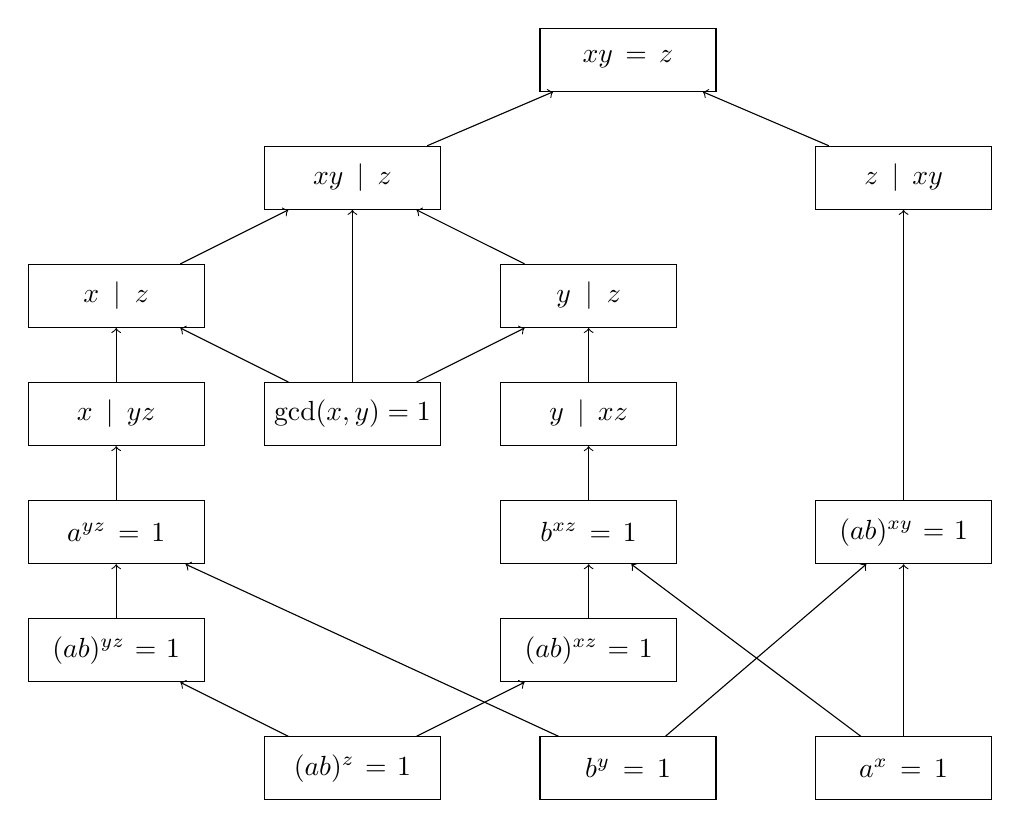
\begin{tikzpicture}[every node/.style={rectangle, draw, text width=2cm,text centered,minimum height=0.8cm}]
  \node (ass_x) at (12, 0) {$a^x=1$};
  \node (ass_y) at (8.5, 0) {$b^y=1$};
  \node (ass_z) at (5, 0) {$(ab)^z=1$};
  \node (abyz)  at (2, 1.5) {$(ab)^{yz}=1$};
  \node (abxz)  at (8, 1.5) {$(ab)^{xz}=1$};
  \node (ayz)   at (2, 3) {$a^{yz}=1$};
  \node (bxz)   at (8, 3) {$b^{xz}=1$};
  \node (abxy)  at (12, 3) {$(ab)^{xy}=1$};
  \node (xyz)   at (2, 4.5) {$x \mid yz$};
  \node (yxz)   at (8, 4.5) {$y \mid xz$};
  \node (ass_g) at (5, 4.5) {$\gcd(x,y)=1$};
  \node (xz)    at (2, 6) {$x \mid z$};
  \node (yz)    at (8, 6) {$y \mid z$};
  \node (xyz_)  at (5, 7.5) {$xy \mid z$};
  \node (zxy)   at (12, 7.5) {$z \mid xy$};
  \node (goal)  at (8.5, 9) {$xy = z$};

  \draw[->] (ass_x) -- (abxy);
  \draw[->] (ass_x) -- (bxz);
  \draw[->] (ass_y) -- (abxy);
  \draw[->] (ass_y) -- (ayz);
  \draw[->] (ass_z) -- (abyz);
  \draw[->] (ass_z) -- (abxz);
  \draw[->] (abyz) -- (ayz);
  \draw[->] (abxz) -- (bxz);
  \draw[->] (ayz) -- (xyz);
  \draw[->] (bxz) -- (yxz);
  \draw[->] (abxy) -- (zxy);
  \draw[->] (xyz) -- (xz);
  \draw[->] (yxz) -- (yz);
  \draw[->] (ass_g) -- (xz);
  \draw[->] (ass_g) -- (yz);
  \draw[->] (xz) -- (xyz_);
  \draw[->] (yz) -- (xyz_);
  \draw[->] (ass_g) -- (xyz_);
  \draw[->] (xyz_) -- (goal);
  \draw[->] (zxy) -- (goal);
\end{tikzpicture}
\caption{証明の流れ}
\label{fig:element_order}
\end{center}
\end{figure}
\end{prProof}

\subsubsection{\rProp{primitive_root_exists}の証明}
\begin{Prop}{}{polynomial_root_n}
$p$を素数とする。
$\mathbb{Z}_p^*$を係数とする$n$次合同式の根は高々$n$個である。
\end{Prop}

\begin{prProof}{polynomial_root_n}
$f(n)$を$n$次合同式とする。
$f(x_0)=0$となる$x_0$が存在したとすると、\rTheo{polynomial_remainder_theorem}より
\begin{align*}
f(x) = (x-x_0)g(x) + f(x_0) = (x-x_0)g(x)
\end{align*}
もし、$x_0$以外の根$x_1$が存在すれば
\begin{align*}
0 = f(x_1) = (x_1-x_0)g(x_1)
\end{align*}
となるが、$x_1-x_0$は$p$で割り切れないから、$g(x_1)=0$。
つまり、$x_1$は$g(x)$の根でなければならない。

以上を念頭に置いて数学的帰納法を使う。

$n=1$のとき、$ax+b\equiv0\pmod{p}$はただ1つの根を持つ。
これは、\rProp{inverse_element_not_exists}からも分かる。

$n=k$のとき、$k-1$次合同式$g(x)$の根は高々$k-1$個であると仮定する。
$f(x)$の根は$x_0$以外は$g(x)$の根しかないので、$f(x)$の根は高々$k$個である。

よって題意は示された。
\end{prProof}

\begin{Lemm}{}{totient_function_multiplicative}
Eulerの$\varphi$関数は乗法的である。つまり、互いに素な$m,n$について、
\begin{align*}
\varphi(mn) = \varphi(m)\varphi(n)
\end{align*}
である。
\end{Lemm}

\begin{Lemm}{}{totient_function_even}
$n>2$のときEulerの$\varphi$関数$\varphi(n)$は偶数である。
\end{Lemm}

\begin{lmProof}{totient_function_even}
Eulerの$\varphi$関数が乗法的であることに注意する(\rLemm{totient_function_multiplicative})。
素数$p$に対して
\begin{align*}
\varphi(p^k) = p^{k-1}(p-1)
\end{align*}
であるから、$n$の素因数に奇素数があれば$(p-1)$が偶数になるので$\varphi(n)$は偶数になる。
また、$n$の因数に$2^k$(ここで$k>1$)があれば、$p^{k-1}$が偶数になるので$\varphi(n)$は偶数になる。
\end{lmProof}

\begin{Prop}{}{primitive_root_search_2p}
奇素数$p$、正整数$k$とし、$p^k$を法とする原始根を$g$とする。
$g$と$g+p^k$のうち、奇数である方が$2p^k$を法とする原始根である。
\end{Prop}

\begin{prProof}{primitive_root_exists}
2以上の自然数を次のように分割し、それぞれに原始根が存在する、あるいは存在しないことを示す。
\begin{enumerate}
 \item 2,4
 \item $2^k$。ただし、$k>2$
 \item 奇素数$p$
 \item $p^k$。ただし、$p$は奇素数で、$k>1$
 \item $2p^k$。ただし、$p$は奇素数で、$k\ge1$
 \item $mk$。ただし、$m$と$k$は互いに素で、$m>2, k>2$
\end{enumerate}

\noindent\textbf{2,4の場合}

$n=2,4$のとき、$g=1,3$がそれぞれの原始根である。

\noindent\textbf{$2^k$の場合}

どんな$a\in\mathbb{Z}_{2^k}^*$の位数も$\varphi(2^k)=2^{k-1}$未満であることを示す。
より具体的には、$a^{2^{k-2}}\equiv1\pmod{2^k}$を示せば、$a$の位数は高々$2^{k-2}$であり、$2^{k-1}$未満であることが分かって、原始根は存在しない。
$a$は奇数だから$a=2t+1$と書き直し、数学的帰納法を用いよう。

$k=3$のとき、
\begin{align*}
(2t + 1)^2 = 4t^2 + 4t + 1 = 4t(t+1) + 1 = 8T + 1 \equiv 1 \pmod{2^3}
\end{align*}
となり成立($t, t+1$のどちらかは偶数だから$4t(t+1)$は8で割り切れる)。

$k=m$のとき、$(2t+1)^{2^{m-3}}=2^{m-1}T+1$を仮定すると、
\begin{align*}
(2t + 1)^{2^{m-2}} = (2^{m-1}T+1)^2 = 2^{2(m-1)}T^2 + 2^mT + 1 = 2^m(2^{m-2}T^2 + T) + 1 \equiv 1 \pmod{2^m}
\end{align*}
となり、$a^{2^{k-2}}\equiv1\pmod{2^k}$が示された。
よって、原始根は存在しない。

\noindent\textbf{奇素数$p$の場合}

素数$p$に対して$p-1=\prod_{i=1}^kq_i^{e_i}$と素因数分解できるとする。
\rProp{polynomial_root_n}より、$(p-1)/q_i$次方程式
\begin{align*}
x^{(p-1)/q_i} \equiv 1 \pmod{p}
\end{align*}
を満たさない$X_i\in\mathbb{Z}_p^*$が存在する。
$Y_i=X_i^{(p-1)/q_i^{e_i}}$と置くと、
\begin{align*}
Y_i^{q_i^{e_i}} &\equiv X^{p-1} \equiv 1 \pmod{p}\\
Y_i^{q_i^{e_i-1}} &\equiv X^{(p-1)/q_i} \not\equiv 1 \pmod{p}
\end{align*}
を得る。
上式はFermatの小定理(\rTheo{Fermats-little-theorem})から得られるし、下式は$X$の前提条件を思い返せば当然の結論だ。
このことから$\mbox{ord}(Y_i)=q_i^{e_i}$を得るが、これはすべての$p-1$の素因数に言える。
そこで、\rProp{element_order}の3を適用すると、
\begin{align*}
\mbox{ord}(Y_1Y_2\cdots Y_k) = q_1^{e_1}q_2^{e_2} \cdots q_k^{e_k} = p-1
\end{align*}
を得る。
よって、$\prod_{i=1}^k Y_i$は$p$を法とする原始根である。

\noindent\textbf{$p^k$の場合}

\rProp{primitive_root_search}より原始根が存在する。

\noindent\textbf{$2p^k$の場合}

\rProp{primitive_root_search_2p}より原始根が存在する。

\noindent\textbf{$mk$の場合}

$mk$(ただし、$m$と$k$は互いに素で、$m>2, k>2$)のとき、\rLemm{totient_function_even}より$\varphi(m),\varphi(k),\varphi(mk)$は偶数であるから、それぞれを2で割っても問題ない。
最終的に、任意の$a\in\mathbb{Z}_n^*$に対して
\begin{align*}
a^{\frac{\varphi(mk)}{2}} \equiv 1 \pmod{mk}
\end{align*}
を示す。
これによって、$a$の位数は$\varphi(mk)$未満であることが分かり、原始根は存在しないと結論付けられる。
それには、$\bmod{m},\bmod{k}$それぞれにおける$a^{\varphi(mk)/2}$を評価してみる。
\rLemm{totient_function_multiplicative}より、$\varphi(mk)=\varphi(m)\varphi(k)$であることを思い出すと、
\begin{align*}
a^{\frac{\varphi(mk)}{2}} &= (a^{\varphi(m)})^{\frac{\varphi(k)}{2}} \equiv 1 \pmod{m}\\
a^{\frac{\varphi(mk)}{2}} &= (a^{\varphi(k)})^{\frac{\varphi(m)}{2}} \equiv 1 \pmod{k}
\end{align*}
となって、$a^{\varphi(mk)/2}\equiv1\pmod{m}$および$a^{\varphi(mk)/2}\equiv1\pmod{k}$を得る。
この2式から、\rTheo{chinese_remainder_theorem}より$a^{\varphi(mk)/2} \equiv 1 \pmod{mk}$が得られる。
\end{prProof}


\newpage
\printindex
\bibliographystyle{plain}
\bibliography{ref}
\end{document}
